\documentclass[tese,capa,english]{texufpel}

\usepackage[utf8]{inputenc} % acentuacao
\usepackage{graphicx} % para inserir figuras
\usepackage{subfigure}
\usepackage[alf,abnt-emphasize=bf, abnt-etal-list=0,bibjustif]{abntex2cite}
\usepackage[table]{xcolor}
\usepackage{booktabs}
\usepackage{tabularx} %breakline in table
\usepackage{amsmath,amssymb,amsfonts,flushend}
\usepackage{algorithm}
\usepackage[noend]{algpseudocode}
\usepackage{listings}
\usepackage{courier}
\usepackage{pdfpages}
\usepackage[activate={true,nocompatibility},final,tracking=true,kerning=true,spacing=true,factor=1100,stretch=10,shrink=10]{microtype}

\microtypecontext{spacing=nonfrench}
\hypersetup{
	pdfauthor={Douglas Pereira Pasqualin}, 
	pdftitle={Sharing-Aware Thread Mapping in Software Transactional Memory},
	pdfsubject={PhD Thesis}, 
	pdfdisplaydoctitle=true,
    pdfkeywords={Software Transactional Memory, Sharing-aware, Thread Mapping, Communication}, 
    pdfcreator={LaTeX, using PPGC/UFPel class}, 
	pdfnewwindow=true,
	bookmarksopen=false,
    pdfstartview={Fit}, 
	hidelinks, % Remove coloração e caixas
	unicode=true,   %Permite acentuação no bookmark
	linktoc=all %Habilita link no nome e página do sumário
}

\pdfinfo{
	/Institution (Universidade Federal de Pelotas)
	/Course (Programa de Pós-Graduação em Computação)
	/Advisor (André Rauber Du Bois)
    /Co-Advisor-1 (Matthias Diener)
    /Co-Advisor-2 (Maurício Lima Pilla)
    /Defense-Date (28 April 2021)
}

\renewcommand*{\backref}[1]{}
\renewcommand*{\backrefalt}[4]{%
	\ifcase #1 \relax%
		\or         (Cited on page~#2).%
		\else      (Cited on pages~#2).%
	\fi
}

\definecolor{myBlue}{HTML}{0000e6}
\definecolor{myGray}{HTML}{969696}
\definecolor{myCyan}{HTML}{2e92c7}
\lstdefinelanguage{STM}
{
	basicstyle=\linespread{0.95}\ttfamily\normalsize,
	numberstyle=\tiny,
	keywords=[1]{foreach, if, else, in, int, void, long, typedef, struct, case, break, switch},
	keywordstyle=[1]\color{myBlue}\ttfamily,
	keywords=[2]{T, address_entry,  NUM_THREADS, HASH_TABLE_SIZE},
	keywordstyle=[2]\color{myCyan}\ttfamily,
	keywords=[3]{volatile, unsigned, \&\&},
	keywordstyle=[3]\color{black}\bfseries,	
	commentstyle=\color{myGray}\ttfamily,
	morecomment=[s]{/*}{*/},
	morestring=[b]",
	showstringspaces=false,
	sensitive=false,
	numbers = left, 
	breaklines=true,
	numbersep=5pt,
	xleftmargin=2em,
	frame=lines,    
}
\lstset{aboveskip=-5pt,belowskip=-5pt}

\newenvironment{conditions}
{\par\vspace{\abovedisplayskip}\noindent\begin{tabular}{>{$}l<{$} @{${}={}$} l}}
	{\end{tabular}\par\vspace{\belowdisplayskip}}

\newcommand{\thNumber}{num\_threads}

\newcommand{\halfPage}{0.47}
\newcommand{\oneQPage}{0.23}
\newcommand{\oneTPage}{0.31}
\newcommand{\oneFPage}{0.175}
\newcommand{\fullImageWidth}{0.95}

%\newcommand{\todo}[1]{\textbf{\color{red}{TODO: #1}}}
%\newcommand{\new}[1]{\textbf{\color{blue}{#1}}}

\newcommand{\citeNamesYearPar}[1]{\citeauthoronline{#1}~\citeyearpar{#1}}

\makeatletter
\algnewcommand{\LineComment}[1]{\Statex \hskip\ALG@thistlm \textcolor{myCyan}{ \(\triangleright\) #1}}
\renewcommand\algorithmiccomment[1]{\textcolor{myCyan}{\hfill\(\triangleright\) #1}}

\makeatother

\unidade{Technology Development Center}
\programa{Graduate Program in Computing}
\curso{Computer Science}

\unidadeeng{Technology Development Center}
\programaeng{Postgraduate Program in Computing}
\cursoeng{Computer Science}

\title{Sharing-Aware Thread Mapping in Software Transactional Memory}

\author{Pasqualin}{Douglas Pereira}
\advisor[Dr.]{Du Bois}{André Rauber}
\coadvisor[Dr.]{Diener}{Matthias}
\coadvisor[Dr.]{Pilla}{Maurício Lima}

%Palavras-chave em EN_US
\keyword{Software Transactional Memory}
\keyword{Sharing-aware}
\keyword{Thread Mapping}
%\keyword{Data mapping}
\keyword{Communication}

%Palavras-chave em PT_BR
\keywordeng{Memória Transacional em Software}
\keywordeng{Sensibilidade ao compartilhamento}
\keywordeng{Mapeamento de thread}
%\keywordeng{Mapeamento de dado}
\keywordeng{Comunicação}

\begin{document}

\maketitle 

\sloppy

%\fichacatalografica
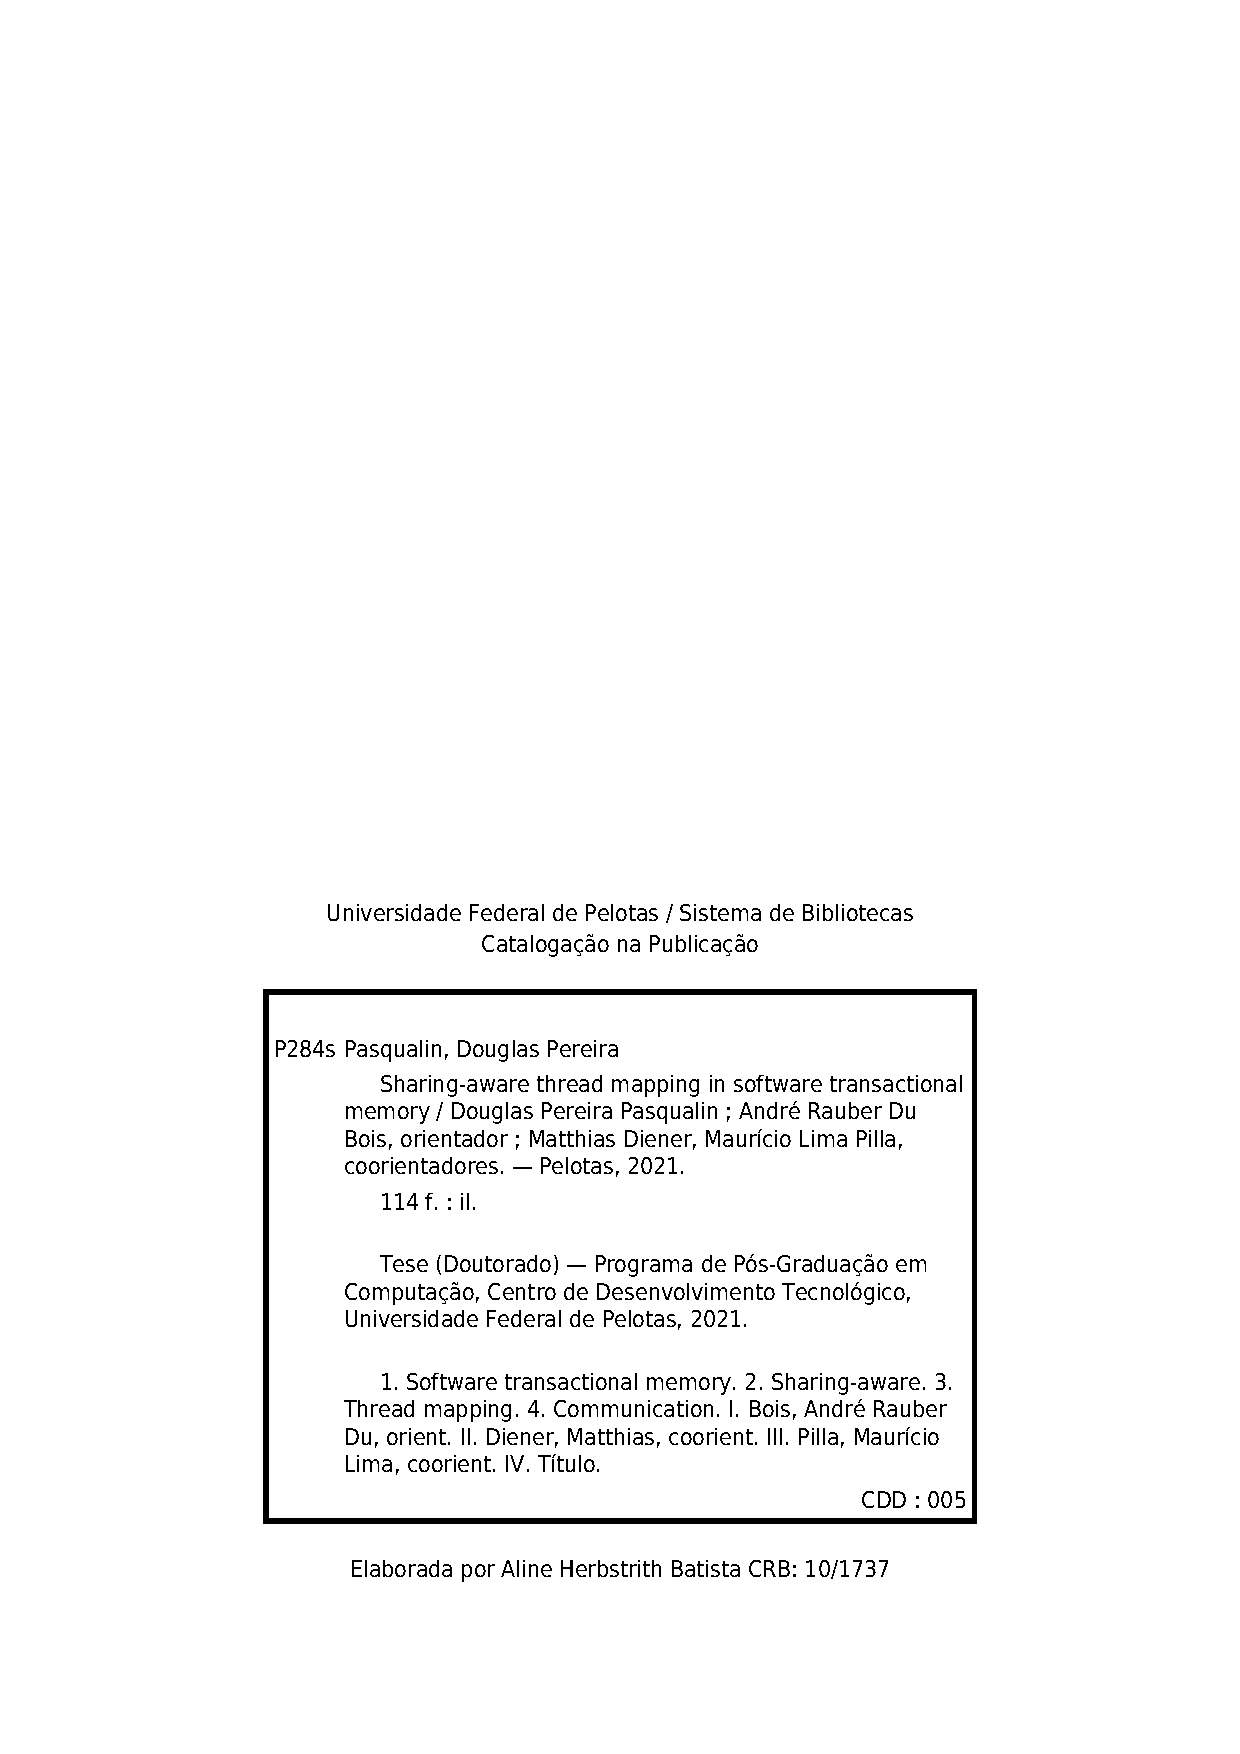
\includepdf{ficha.pdf}

%Composição da Banca Examinadora
\begin{aprovacao}{28 April 2021} %data da banca por extenso
\noindent Dr. André Rauber Du Bois (advisor)\\
PhD in Computer Science from the Heriot-Watt University, Scotland.\\[1cm]

%\noindent Dr. Matthias Diener (coadvisor)\\
%PhD in Computer Science from the Technische Universität Berlin, Germany.\\[1cm]

%\noindent Dr. Maurício Lima Pilla (coadvisor)\\
%PhD in Computer Science from the Federal University of Rio Grande do Sul, Brazil.\\[1cm]

\noindent Dr. Laércio Lima Pilla\\
PhD in Computer Science from the Federal University of Rio Grande do Sul (UFRGS), Brazil and Université Grenoble Alpes, France.\\[1cm]

\noindent Dr. Alexandro José Baldassin \\
PhD in Computer Science from the State University of Campinas (UNICAMP), Brazil \\[1cm]

\noindent Dr. Gerson Geraldo Homrich Cavalheiro\\
PhD in Informatique Systèmes et Communications from the Institut National Polytechnique de Grenoble, France.
\end{aprovacao}


\begin{dedicatoria}
	\begin{flushleft}	
		%\sffamily\itshape 
	%	\begin{hyphenrules}{nohyphenation}
			This is dedicated to my wife Daiane and my son Nicolas, for their endless love and encouragement.
	%	\end{hyphenrules}
	\end{flushleft}		
\end{dedicatoria}

%Opcional
\begin{agradecimentos}
	Finally, it is time to write this hard part of the thesis. The acknowledgments! Although it is an optional element of the document, I think that it should be mandatory. It is nearly impossible to imagine developing a PhD thesis alone. Many people work together and backstage, but all are fundamental to reach the final objective. Now it is time to thank them all.

\vspace*{0.5cm}

Firstly, I would like to thank my advisor team. Indeed, I do not have just an advisor and a co-advisor, but a team of three advisors. Each one started in a distinct phase of this thesis. So, I thank you, Prof. Dr. André Du Bois, for accepting me as a PhD student. Also, for your support and confidence in me. Prof. Dr. Maurício Pilla, for sharing profound knowledge and guidance during my initial studies on the thesis subject. Finally, Dr. Matthias Diener, I have no words to thank you for all your support. Our contact started with a simple question about your work on Facebook and finished with you being officially my co-advisor. My sincerely \textit{Herzlichen Dank}.

\vspace*{0.5cm}

I also would like to thank another team that was always working backstage: my family! Especially my wife Daiane, my son Nicolas and my mom Maria. Thank you for the support and encouragement during these four long years, including giving me the strengths to continue when sometimes I thought that I would not be able to make it! But I did it! This achievement is also yours.

\vspace*{0.5cm}

Lastly, I would like to thank my employer (CPD and UFSM) to grant me the privilege of getting a license of my professional activities. Hence, it was possible to dedicate my full time to my PhD studies.

\vfill
\textit{This study was financed in part by the Coordena\c{c}\~ao de Aperfei\c{c}oamento de Pessoal de N\'ivel Superior - Brasil (CAPES) - Finance Code 001 and PROCAD/LEAPaD}

\end{agradecimentos}

%Opcional
\begin{epigrafe}
	\begin{flushright}	
%	\begin{hyphenrules}{nohyphenation}		
			``Accessing memory is more like mailing a letter than making a phone call''
			\vspace*{0.5cm}
			\textsc{\\(The Art of Multiprocessor Programming, page 471)}
%	\end{hyphenrules}		
	\end{flushright}	
\end{epigrafe}

%Resumo em inglês (no maximo 500 palavras)
\begin{abstract}
Software Transactional Memory (STM) is an alternative abstraction for thread synchronization in parallel programming. One advantage is simplicity since it is possible to replace the use of explicit locks with atomic blocks, while the STM runtime is responsible to ensure a consistent execution, for instance, without deadlocks and race conditions. Regarding STM performance, many studies already have been made focusing on reducing the number of transactional aborts and conflicts. However, in current multicore architectures with complex memory hierarchies, it is also important to consider where the memory of a program is allocated and how it is accessed. This thesis proposes the use of a technique called \emph{sharing-aware mapping}, which maps threads to cores and memory pages to NUMA nodes based on their memory access behavior to achieve better performance in STM systems. The first major contribution of this thesis is a mechanism to detect sharing behavior directly inside the STM library by tracking and analyzing how threads perform STM operations. The collected information can be used to perform an optimized mapping of the application's threads to cores in order to improve the efficiency of STM operations. The second contribution of this thesis is the characterization of the sharing behavior of STM applications by using information extracted from the STM runtime, providing information to guide thread mapping based on their sharing behavior. The third contribution is a mechanism to perform sharing-aware thread mapping in STM applications. We first introduce \emph{Static-SharingAware}~(SSA), which map threads to cores based on a previous analysis of the sharing behavior of STM applications. Next, we introduce STMap, an online, low overhead mechanism to detect the sharing behavior and perform the mapping directly inside the STM library, by tracking and analyzing how threads perform STM operations during the execution. In experiments with the STAMP benchmark suite and synthetic benchmarks, both mechanisms showed performance gains when compared to the default Linux scheduler. %Finally, we show how STMap can be extended to include sharing-aware data mapping.
\end{abstract}

%Resumo em PT-br (sim, está invertido) (no maximo 500 palavras)
\begin{englishabstract}{Mapeamento de \textit{Threads} Baseado em Compartilhamento em Memórias Transacionais em Software}
Memória Transacional em Software (MTS) é uma abstração para a sincronização de \textit{threads} na programação paralela. Uma de suas vantagens é a simplicidade, pois é possível substituir o uso de bloqueios por blocos atômicos. Além disso, a implementação de MTS é responsável por garantir uma execução consistente, por exemplo, sem \textit{deadlocks} ou condições de corrida. Com relação ao desempenho de MTS, existem muitos estudos focados na redução do número de cancelamentos. Contudo, nas atuais arquiteturas \textit{multicore}, com complexas hierarquias de memória, é também importante considerar onde a memória do programa está alocada e como ela é acessada. Esta tese propõe o uso de uma técnica chamada \emph{mapeamento baseado em compartilhamento} a qual consiste em mapear \textit{threads} para núcleos de processamento e páginas de memória para nós NUMA com base no seu padrão de acesso à memória para melhorar o desempenho de aplicações que utilizam MTS. A primeira contribuição desta tese é um mecanismo para detectar o padrão de acesso à memória em bibliotecas de MTS. Ele consiste em rastrear e analisar como \textit{threads} executam operações de MTS. As informações coletadas podem ser utilizadas para criar um mapeamento otimizado de \textit{threads} para núcleos de processamento, com o objetivo de melhorar a eficiência das operações de MTS. A segunda contribuição é a caracterização do padrão de acesso à memória de aplicações que utilizam MTS, fornecendo informações para guiar um mapeamento de \textit{threads} com base no padrão de compartilhamento da aplicação. A terceira contribuição é um mecanismo para efetuar um mapeamento de \textit{threads} baseado em compartilhamento para aplicações que utilizam MTS. Primeiramente é apresentado \emph{Static-SharingAware}~(SSA), que baseado em uma análise prévia do padrão de compartilhamento da aplicação, mapeia \textit{threads} para núcleos de processamento de forma estática. Após, é apresentado STMap, um mecanismo que opera dinamicamente e com baixa sobrecarga, com o objetivo de detectar o padrão de acesso à memoria e efetuar o mapeamento de \textit{threads} durante a execução do programa. Em experimentos com o benchmark STAMP e outras aplicações sintéticas, ambos mecanismos apresentaram ganhos de desempenho quando comparados com o escalonador padrão do Linux. %Por fim, é apresentado como o STMap pode ser estendido para incluir o mapeamento de dados basedo em compartilhamento.

\end{englishabstract}

%Lista de Figuras
\listoffigures

%Lista de Tabelas
\listoftables

%lista de abreviaturas e siglas
\begin{listofabbrv}{LO-SER}
	\item[ACC]   		Adaptive Concurrency Control
	\item[ATS]	 		Adaptive Transaction Scheduling
	\item[AR]			Abort Ratio
	\item[BAT] 			Best Alternative Transaction
	\item[CAR]   		Collision Avoidance and Resolution
	\item[CB]			Contention Bit
%	\item[CC]   		Concurrency Control
	\item[CDSM]		Communication Detection in Shared Memory
	\item[CFS]			Completely Fair Scheduler
	\item[CI]    		Contention Intensity
	\item[CL]			Concurrency Level
	\item[CM]    		Contention Manager
	\item[CMP] 		Chip Multiprocessor
	\item[CP]			Contention Predictor
	\item[CPU]			Central Processing Unit
	\item[CR]			Commit Ratio
	\item[DA]			Distinct Addresses
	\item[DoT]			Dominant Thread
	\item[DS]			Dynamic Serializer
	\item[DVFS]      Dynamic Voltage and Frequency Scaling
	\item[F2C2] 		Flux-based Feedback-driven Concurrency Control
	\item[GC] 			Garbage Collector
	\item[GPU]          Graphics Processing Unit
	\item[HPC]			High Performance Computing
	\item[HTM]			Hardware Transactional Memory
	\item[IBS]			Instruction-Based Sampling
	\item[kMAF]			kernel Memory Affinity Framework
	\item[LLC] 				Last-Level Cache
	\item[LO-SER]		Low-Overhead Serializing Algorithm
	\item[LSA]          Lazy Snapshot Algorithm 
	\item[LUTS]			Light-Weight User-Level Transaction Scheduler
	\item[MAi]			Memory Affinity Interface
	\item[MI]			Mapping Interval
	\item[ML]			Machine Learning	
	\item[MPI] 			Message Passing Interface
	\item[MSE]			Mean squared error
%	\item[Mutex] 		Mutual Exclusion
	\item[NPB]			NAS Parallel Benchmark
	\item[NUMA]  		Non-Uniform Memory Access
%	\item[NumaMMa] NUMA MeMory Analyzer
%	\item[OS]			Operating System
	\item[PEW]			Percentage of the Effective Work
	\item[PoCC]  		P-only Concurrency Controller 
	\item[ProPS] 		Progressively Pessimistic Scheduling
	\item[SC]			Saturating Counter
	\item[SCA]			Speculative Contention Avoidance
	\item[SI]				Sample Interval
%	\item[SD]			Standard Deviation
	\item[SRP] 			Success-Reward Policy
	\item[SSER+]		Stricter Serializability
%	\item[RBTree]		Red-Black Tree
	\item[RS]			Read-set
%	\item[TABARNAC]		Tools for Analyzing the Behavior of Applications Running on NUMA ArChitecture
	\item[TBB]			Threading Building Blocks
	\item[TCR]	 		Transaction Commit Ratio
	\item[TCP]			Transmission Control Protocol
	\item[TLB] 			Translation Lookaside Buffer
	\item[TM]    		Transactional Memory	
	\item[SOA]			Steal-on-Abort
	\item[SSA]			Static-SharingAware
	\item[STAMP]		Stanford Transactional Applications for Multi-Processing
	\item[STM]   		Software Transactional Memory
	\item[UMA]		Uniform Memory Access
	\item[VIT]			Very Important Transaction
	\item[WACC] 		Weighted Adaptive Concurrency Control
	\item[WS] 			Write-set
%	\item[WW] 			Wasted Work
\end{listofabbrv}

%Sumario
\tableofcontents

%Add chaptes
\chapter{Introduction}

At the beginning of the year 2000, multicore processors started to be produced. This decision was taken due to the microarchitectural limitations and, higher power consumption and heat dissipation involved on improving the performance of a single CPU~\cite{Trono:2015}. Since then, the number of cores in a single chip is growing every year. Today, desktops and even cellphone processors are multicore. Besides, servers normally have many processors and each one is multicore. 

The simplest architecture for multiprocessors systems are based on a single bus, i.e., one or more processors and memory modules use the same bus for communication. In this architecture, every memory word can be read with the same latency. Hence, they are named UMA (Uniform Memory Access). However, these architectures have a scalability problem as the number of CPUs grow, as all communication needs to pass by the single bus.

One alternative is to replace the single bus with multiple nodes, where each node is a multiprocessor connected directly to a local memory module \cite{Gaud:2015}. These architectures are called NUMA (Non-Uniform Memory Access) and are becoming dominant in servers~\cite{Calciu:2017}. In NUMA machines, programs have access to the entire memory. In a transparent way, data can be stored in the local node or in a node that belongs to other processor (remote node). Interconnect links between nodes are asymmetric and have different bandwidths~\cite{Lepers:2015}. Hence, the location of the data plays an important role in the performance.


Accessing a remote node implies higher latency, making the access time non-uniform, i.e., depends on the location of the data. 

In order to better exploit the parallelism available in these modern architectures,  software must be parallel and scalable \cite{Grahn:2010}. An important issue that arises in parallel programming is thread synchronization, and it is the major cause that prevents the scalability of applications~\cite{David:2013}. Synchronization is necessary when multiple concurrent threads need to access at the same time a shared variable and, at least one thread needs to write to this shared variable. If there is no synchronization, a race condition can happen~\cite{Netzer:1992}, possibly leading to non-deterministic results~\cite{Trono:2015}. The block of code that needs to be protected in order to not be accessed at the same time by different processes is called \emph{critical section} \cite{Raynal:2013}. 

Mutual-exclusion locks are one of the most used abstractions to protect critical sections~\cite{Fraser2007}. However, the semantics of locks is not intuitive.  Programmers need to explicitly acquire and release  locks, making the source code hard to read and debug~\cite{Anthes:2014}. Besides, if more than one lock was acquired in a critical section, they need to be released in the same order, to avoid \emph{deadlocks}~\cite{Herlihy:2008}. The performance of locks depends on the size of the critical section that it protects. Coarse-grained locks are easy to program but the parallelism is limited~\cite{TL2}. On the other hand, fine-grained locks provide good performance but they are hard to use~\cite{Dice:2007}.

An alternative abstraction to replace mutual-exclusion locks in  parallel programming is the \emph{Transactional Memory} (TM)~\cite{Harris:2010, Grahn:2010}, in which critical-sections are accessed using transactions similar to the ones available in databases. With TM, instead of explicitly acquiring and releasing locks, the programmer only needs to delimit the block of code that he wants to be executed atomically as a transaction. The TM runtime is responsible to ensure a consistent execution, e.g., without deadlocks and race conditions. A transaction that has executed without conflicts can commit, i.e., update the memory with the new values. If a conflict was detected an abort is executed and a transaction is reinitialized until a commit is possible. Thus, an impression of atomicity is given to the programmer. Although there are TMs implemented in hardware (HTM) and in software (STM), this thesis focuses on the study of STM, where transaction consistency is guaranteed by a software library. An advantage of an implementation in software is that it is more flexible and not dependent on hardware. Also, it does not have the same resource limitations as in hardware~\cite{Grahn:2010}.%. Even if hardware support is available, implementation in software still be necessary for larger transactions~\cite{Anthes:2014}.

\section{Motivation}\label{sect:motivation}
%Many researches on schedulers
%Current microarchitectures placement of threads and data is important for performance
%Try to use sharing-aware mapping inside STM, since STM has precise information about shared variables

There are many compilers and programming languages that already support transactional memory constructs, such as C++ (since the standard C++11\footnote{\url{https://gcc.gnu.org/wiki/TransactionalMemory}}), Haskell, Scala and .NET Framework~\cite{Gramoli:2017}. Besides, some researches already showed that STM can outperform locks in some scenarios \cite{Dice:2007, STMNOTToy}. Unfortunately, there are scenarios where the overhead added by the management of internal metadata of the STM or a high number of aborts, limits good performance~\cite{Gramoli:2014}. Due to these limitations, improving performance of STM is an active research area. 
There are several proposals for increasing the performance of STM systems. However, the majority of them focus on reducing the number of conflicts (transactional aborts). One technique is the use of a transactional scheduler, acting proactively, using heuristics to prevent conflicts and to decide \emph{when} and \emph{where} a transaction should be executed~\cite{Sanzo:2017}.

Current multicore architectures have complex memory hierarchies and different latencies for memory accesses. Hence, a thread placement that improves the use of memory controllers and data locality is important to achieve good performance. A technique called \emph{sharing-aware mapping}\footnote{This research field is also known as topology-aware mapping~\cite{Jeannot:2013,Unat:2017}.}~\cite{Cruz:2018} aims to map threads to cores and memory pages to NUMA nodes considering their memory access behavior. Since STM is used to synchronize data accessed by multiple threads, an efficient mapping will help to make better usage of caches and memory controllers, hence improving the overall performance. Besides, STM provides interesting mapping opportunities since the STM runtime has precise information about memory areas that are shared between threads, their respective memory addresses, and the intensity with which they are accessed by each thread. Hence, contrary to prior works on sharing-aware thread mapping, it is not necessary to keep track of all memory access of the applications, only the STM accesses. Therefore, the proposed mechanism will have a low overhead and can perform sharing-aware thread mapping accurately for STM applications.


\section{Contributions}

%The main objective of this thesis is to improve the performance of STM applications by using the information about transactional shared variables inside the STM runtime to performing an efficient sharing-aware mapping. 
The main objective of this thesis is to investigate the use of sharing-aware mapping in the context of STM. %The main intuition is that STM has precise information about shared variables and has native access to all information need to characterize the sharing behavior, i.e., accessed memory address and the intensity with which each thread accesses them. 
	Contrary to previous sharing-aware mapping proposals that rely on memory traces of the entire application, our proposal has lower overhead and better accuracy because only memory accesses that are in fact shared between threads are traced. Beyond that, this sharing-aware mapping will improve the overall performance of STM applications by improving the cache usage and interconnection traffic. More specifically, this thesis makes the following contributions:

\begin{itemize}
	\item We developed a low overhead mechanism to \textbf{detect the sharing behavior of STM applications}, by tracking and analyzing how threads perform STM operations~(Chapter~\ref{chap:mechanism}).
	
	\item We made an \textbf{in-depth characterization of STM applications}, regarding memory access behavior, using the proposed mechanism. This characterization is used to define the suitability for a thread mapping based on communication behavior and defining which type of mapping policy is more appropriate (static or dynamic)~(Chapter~\ref{chap:charact}).
	
	\item We show how a \textbf{static thread mapping} (where threads are mapped to cores at the beginning of execution, and never migrated) is sufficient to improve the overall performance of the majority of STM applications~(Chapter~\ref{chap:sharAwareThreadMap}, Section~\ref{sect:staticThreadMap}). 
	
	\item We extend the proposed mechanism to perform \textbf{online detecting sharing behavior and mapping}. %detect the sharing behavior of STM application to perform thread mapping during the execution of the STM application~(online). 
	We developed a heuristic to disable the mechanism if it determines that the application will not benefit from a new thread mapping~(Chapter~\ref{chap:sharAwareThreadMap}, Section~\ref{sect:onlineThreadMapping}). 
	
%	\item A heuristic to disable the online mechanism, if it predicts no improvements of a new mapping. 
%	\item We show how the proposed mechanism to perform online sharing-aware thread mapping can be extended to include \textbf{sharing-aware data mapping}~(Appendix~\ref{chap:sharAwareDataMap}).
\end{itemize}


\section{Publications}

The following papers were published during the PhD program and contain material that is relevant to this thesis:

\begin{enumerate}
	\item \underline{Douglas P. Pasqualin}, Matthias Diener, André R. Du Bois, Maurício L. Pilla. \textbf{``Thread Affinity in Software Transactional Memory.''}  19th International Symposium on Parallel and Distributed Computing (ISPDC), July 2020 \cite{Pasqualin:2020}.
	
	\item \underline{Douglas P. Pasqualin}, Matthias Diener, André R. Du Bois, Maurício L. Pilla. \textbf{``Online Sharing-Aware Thread Mapping in Software Transactional Memory.''}  32nd International Symposium on Computer Architecture and High Performance Computing (SBAC-PAD), September 2020 \cite{Pasqualin:2020:2}.
	
	\item \underline{Douglas P. Pasqualin}, Matthias Diener, André R. Du Bois, Maurício L. Pilla. \textbf{``Characterizing the Sharing Behavior of Applications using  Software Transactional Memory.''} Benchmarking, Measuring, and Optimizing (Bench'20). November 2020. (\textbf{Best Paper Award} and \textbf{Award for Excellence for Reproducible Research}) \cite{Pasqualin:Bench}.
\end{enumerate}

The following papers were also submitted for publication and are currently under peer-review:

\begin{enumerate}
	\item \underline{Douglas P. Pasqualin}, Matthias Diener, André R. Du Bois, Maurício L. Pilla. \textbf{``STMap: Sharing-Aware Thread Mapping in Software Transactional Memory.''} Journal of Parallel and Distributed Computing (JPDC).
	
	\item \underline{Douglas P. Pasqualin}, Matthias Diener, André R. Du Bois, Maurício L. Pilla. \textbf{``Sharing-Aware Data Mapping in Software Transactional Memory.''} SAMOS XXI - International Conference on Embedded Computer Systems: Architectures, Modeling and Simulation. 
\end{enumerate}


\section{Document organization}

The remainder of this thesis is organized as follows. Chapter~\ref{chap:background} presents the background of different topics used in this thesis, such as TM and sharing-aware mapping. Chapter~\ref{chap:related} presents the works related to the thesis subject. Also, we discuss the differences between our contributions with related work. Chapter~\ref{chap:mechanism} presents the first contribution of this thesis, i.e, a mechanism to detected the sharing behavior of STM applications, by tracking and analyzing how threads perform STM operations. Chapter~\ref{chap:charact} uses the proposed mechanism of Chapter~\ref{chap:mechanism} to perform an in-depth characterization of \texttt{STAMP}, a frequently used TM benchmark suite, regarding memory access behavior. It includes information about the suitability for thread mapping of each \texttt{STAMP} application, its communication pattern, and its dynamic behavior, among others. Chapter~\ref{chap:sharAwareThreadMap} shows how to use the proposed mechanism to perform static and online thread mapping based on the memory access behavior of STM operations. %Chapter~\ref{chap:sharAwareDataMap} show how to extend the online thread mapping to include sharing-aware data mapping. 
Finally, Chapter~\ref{chap:conclusion} presents the conclusion and future work. We also included Appendix~\ref{chap:sharAwareDataMap} which shows how to extend the online sharing-aware thread mapping mechanism to include data mapping. 


\chapter{Background}\label{chap:background}

This chapter covers the background on the range of different topics which are important to this thesis. It starts by explaining transactional memory~(Section~\ref{chap:TM}) and sharing-aware mapping~(Section~\ref{sect:sharing-aware}). Benchmarks for STM are briefly described in Section~\ref{sec:STAMP}. We also include a small experiment to show the benefits of sharing-aware thread mapping for STM applications~(Section~\ref{sec:improvements}).

\section{Transactional Memory}\label{chap:TM}

Transactional memory (TM) is an abstraction to synchronize accesses to shared variables. Instead of using locks, the programmer only needs to enclose the critical section in an atomic block, which will be executed as a transaction. The concept of transactions was borrowed from Databases. In fact, the first idea to use Database transactions in programming languages was described by \citeNamesYearPar{Lomet:1977}. Sixteen years later, \citeNamesYearPar{Herlihy:1993} proposed hardware support for TM. The first implementation purely on software (STM) was proposed by \citeNamesYearPar{Shavit:1995} as a flexible alternative not dependent on hardware. There are also hybrid approaches \cite{Damron:2006} that combine implementation both on hardware and software.


\subsection{General Concepts}\label{sec:TMConcepts}

The execution of a transaction needs to be \emph{atomic}. Atomicity requires that a transaction is executed as a whole or it needs to appear as it was never executed \cite{Harris:2010, Grahn:2010}. This property is also known as ``all-or-nothing'' \cite{Ozsu:1996}. A transaction \emph{commits} if executed without conflicts, hence all operations and results are made visible to the rest of the system \cite{Grahn:2010}. If conflicts are detected, a transaction \emph{aborts}, i.e., all operations are discarded, and the transaction needs to restart until a commit is possible. This idea is associated with another important property called \emph{isolation}: all memory updates of a running transaction can not be visible to other transactions before a commit.

The sequence of operations performed by all transactions in a given execution is called \emph{history} \cite{Opacity}. If one transaction executes only after the end of the other they are serial, otherwise \emph{concurrent} \cite{Harris:2010}. If they are concurrent, conflicts could occur between them. A conflict occurs when two transactions perform operations in the same memory location, and at least one of these operations is a write. 

As transactions can execute concurrently, correctness criteria were proposed to ensure that the TM system produces correct results. One of the most used criteria is \emph{Opacity} \cite{Opacity}, that is an extension of the classical database criteria \emph{Strict Serializability} \cite{Papadimitriou:1979}. Serializability says that the result of executing concurrent transactions in a given history must be equal to a serial execution. \emph{Strict Serializability} says that real-time order must be respected. If $T_1$ finishes before $T_2$ starts, then $T_1$ must occur before $T_2$ in the equivalent serial execution \cite{Harris:2010}. Opacity extends these concepts to aborted transactions, i.e., all transactions in a given history, including aborted, must appear to be executed in a serial order. %There are weaker alternatives proposed after Opacity, for instance, \emph{Virtual World} \cite{VWCFull} and \emph{Stricter Serializability} (SSER+) \cite{Sutra:2018}. 

%%%%%%%%%%%%%%%%%%%%%%%%%%%%%%%%%%%%%%%%%%%%%%%%%%%%%%%%%%%%%%%%%%%%
\subsection{Design Choices}\label{sec:TMDesignChoices}

Although the main purpose of TM is to provide a simple interface to manage accesses to shared resources, its implementation is not trivial. Many different design options are available such as transaction granularity, version management, conflict detection and resolution. The next subsections describe these design options.

\subsubsection{Version Management}\label{sec:versionManag}

TMs use version management of memory locations to manage the writes of concurrent transactions. Two approaches are used \cite{Harris:2010, TinySTM2}:

\begin{itemize}
	\item \textbf{Eager}, \textbf{direct update} or \textbf{write-through}: data is modified directly in memory. Older values are stored in an \emph{undo-log}. In case of an abort the log is used to restore the old values.
	
	\item \textbf{Lazy}, \textbf{deferred update} or \textbf{write-back}: instead of updating data directly in memory, new values are stored in an \emph{redo-log}. During a commit, the log is used to set new values to memory.  In case of an abort, the log is discarded.
\end{itemize}

Eager versioning makes committing faster, whereas lazy versioning makes aborting faster \cite{Grahn:2010}.

\subsubsection{Transaction Granularity}\label{sec:granularity}

The granularity is the dimension used for conflict detection, i.e., the level used for keeping track of memory locations. One option is to use memory \textbf{word} granularity. The main advantage is that no false conflicts happen. However it adds a high overhead in terms of time and space to keep the metadata \cite{Grahn:2010}. \textbf{Object} granularity is most used in object-based languages \cite{CastroPhD:2012}. However it can lead to false conflicts, i.e., transactions accessing the same object but different fields \cite{Larus:2008}. For HTM, \textbf{cache line} granularity is the most suitable~\cite{Grahn:2010}.

\subsubsection{Conflict Detection}\label{sec:conflictDetection}
Similar to version management, there are two approaches to deal with conflict detection between concurrent transactions \cite{Grahn:2010}:

\begin{itemize}
	\item \textbf{Eager}, \textbf{early}, \textbf{pessimistic} or \textbf{encounter-time}: conflicts are verified on each memory location read or written exactly when it occurs. In STM this could be done using locks or version number on memory locations. Thus, to access a value, a transaction needs to acquire its ownership, preventing others from accessing it \cite{Bandeira:2015}.
	
	\item \textbf{Lazy}, \textbf{late}, \textbf{optimistic} or \textbf{commit-time}: conflicts are verified only at commit time. It allows multiple transactions to access shared data and continue executing even if they conflict, as the TM system will detect and resolve them on commit time~\cite[p. 20]{Harris:2010}.
	
	%A transaction must validate all its read set in order to verify if any conflict with other transactions occurred. 
\end{itemize}

These options could be combined, for instance, lazy conflict detection for reads and eager for writes \cite{Bandeira:2015}.

\subsubsection{Conflict Resolution}\label{sec:contetionManager}

All operations executed by a transaction that aborts could be seen as a wasted work \cite{Spear:2009, Ansari:2009:PTM, Zhou:2016}. Thus, the total aborts in an execution have a strong relationship with the final performance. In case of conflicts, choosing which transaction needs to be aborted is a responsibility of the \emph{Contention Manager} (CM) \cite{Yoo:2008}. When two transactions $T_A$ and $T_B$ conflict, the transaction that has detected the conflict, suppose $T_A$, asks  the CM what to do. The actions could be, for instance, abort immediately or wait a determined time, allowing $T_B$ to finish, or force and abort of $T_B$~\cite{Guerraoui:2006}. 
There are many CMs proposed in the literature with different purposes. A few examples of them are \cite{Scherer:2005, Spear:2009, Harris:2010, Grahn:2010}: 
\begin{itemize}
	\item \textbf{Passive}: the transaction that detected the conflict aborts and restart its execution.
	
	\item \textbf{Polite}: the transaction that detected the conflict could abort the conflicting one. However,  aborting is delayed for a period of time, waiting the conflicting transaction to end accessing values. The transaction can also wait for a fixed number of exponentially growing intervals
	before aborting the enemy.
	
	\item \textbf{Karma}: use priorities to define which transaction must abort. The priority is defined by the total of memory locations that a transaction has accessed. The total is cumulative, i.e., taking in consideration all aborts and re-executions.
	
	\item \textbf{Timestamp}: aborts the transaction that started earlier.
	
	\item \textbf{Polka}: a hybrid between \textit{Polite} and \textit{Karma}.
	%As demonstrated in \cite{Scherer:2005}, the CM that achieved best performance were \textit{Polite} and \textit{Karma}. Thus, \textit{Polka} is a hybrid between the two.
\end{itemize}

%%%%%%%%%%%%%%%%%%%%%%%%%%%%%%%%%%%%%%%%%%%%%%%%%%%%%%%%%%%%%%%%%%%%
\subsection{STM Implementation}\label{sec:implementationTM}

The first STM implementations were non-blocking \cite{Shavit:1997}, more specifically obstruction-free \cite{Herlihy:2003_2}. However, according to \citeNamesYearPar{Ennals:2006}, obstruction-free is essential in distributed systems but not appropriate for non-distributed STM. In the same publication, Ennals shows that lock-based STM are simpler to implement and faster. As a consequence many state-of-art STM implementations, for instance, \texttt{TL2} \cite{TL2}, \texttt{TinySTM} \cite{TinySTM2} and \texttt{SwissSTM} \cite{SwissTM} are lock-based.

Other characteristic used in the first implementations was \emph{visible reads}, i.e., all transactions knew who read a specific memory location. To implement this approach it is necessary a list to store all transactions who read a specific memory location. Thus, when a transaction writes new values in memory, it is possible to notify the readers that there is a conflict. The disadvantage of this approach arises when many distinct threads read the same memory location \cite{TinySTM2}. As most workloads are read-intensive, this approach limits the performance~\cite{Sutra:2018}. The opposite solution is to use \emph{invisible reads}, where other threads do not know who read a specific memory location. However, using this approach, a thread could be in an inconsistent state (due to a conflict) and does not know yet. Letting this transaction continue  execution could bring an unwanted result, not guaranteeing Opacity or other consistency. Thus, a solution to using invisible reads is to periodically validate the read set, verifying if the memory locations read are still consistent. On the other hand, this solution is expensive, mainly if a transaction has read many memory locations. This cost keeps growing as the transaction keeps reading different memory locations. This problem is known as \emph{incremental validation} \cite{Harris:2010}.

To use invisible reads without the problem of incremental validation the concept of \emph{global clock} was introduced in an independent way in the algorithms \texttt{TL2} \cite{TL2} and \texttt{LSA} (Lazy Snapshot Algorithm) \cite{Riegel:2006}. The global clock is a counter utilized for versioning memory locations. When a transaction writes new values to  memory, the global clock is incremented and the new clock value is used as a version number for modified memory locations. In STM implementations that use a global clock, transactions still need to validate their read set, but in general, this is necessary only for write transactions during the commit phase. Read only transactions can commit without validation, because  memory location were validated when read. 

\subsubsection{Using a global clock}

This section presents an overview of how an STM implementation that uses a global clock for versioning memory locations works. The operations described are based on algorithms \texttt{TL2}~\cite{TL2} and \texttt{TinySTM}~\cite{TinySTM2}. However, minor details could be different depending on the STM implementation.

\begin{figure}[ht]
	\centering
	\fbox{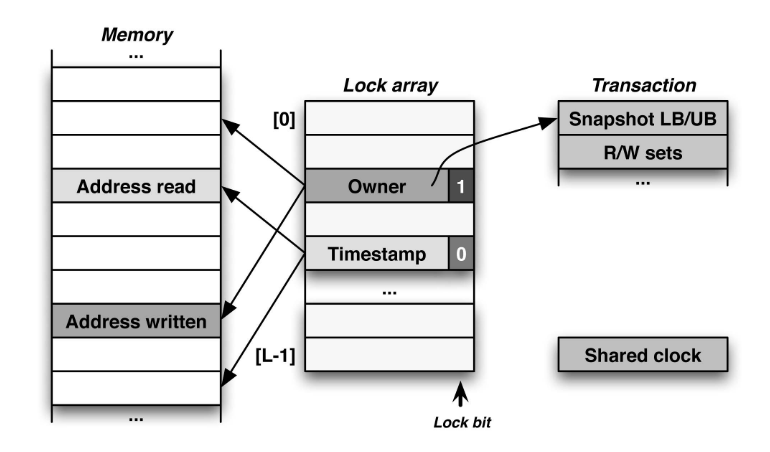
\includegraphics[width=\textwidth]{figures/background/TinySTMDataStructs.png}}
	\caption{Data structures utilized internally by the STM library \texttt{TinySTM}. Source: \cite{TinySTM2}. R/W sets stands for read and write sets. A snapshot corresponds to a range of valid linearization points. LB and UB stand for lower and upper bounds, i.e, the validity range of the snapshot.}
 	\label{fig:TinySTMDataStructs}
\end{figure} 

Figure \ref{fig:TinySTMDataStructs}, represents the internal organization of \texttt{TinySTM}. Each transaction has two internal linked lists, called read-set (RS) and write-set (WS). These lists are utilized to keep track of memory locations read and written by transactions. Another important data structure for STMs, is the lock array, implemented using a hash table. This table is utilized to map memory locations to their related versioned locks. When a versioned lock is locked, its last bit is set to one and the remaining bits contain the owner of the memory location. If the lock is free, it contains the current version of the memory location, also called timestamp (Figure \ref{fig:TinySTMDataStructs}). Some authors call the lock array as \emph{ownership records} (orecs), because it associates memory locations with their current owners \cite{NOrec}.

To summarize, a transaction performs the follow operations. To make it simpler, we do not intent to cover all possible algorithm cases. The main idea is to show the basics of how an STM algorithm works.

\begin{itemize}
	\item \textbf{Begin Transaction}: The current global clock value is copied to a local variable of the transaction. Normally, the variable name is $rv$ which stands for \textit{\textbf{r}ead \textbf{v}ersion}. This value will be utilized to validate reads on memory locations.
	
	%---------------------------------------------------------%
	\item \textbf{Read} or \textbf{Load}: 	With \textbf{eager} version management (Section \ref{sec:versionManag}), the transaction verifies if it owns the lock of the memory location that is being read. If true, it returns directly the value stored in memory. If the lock of the memory location belongs to another transaction, an abort is necessary.  Using \textbf{lazy} version management, the transaction first verifies if the memory location that it wants to read is in their WS. In that case, the transaction has already written to this location and the value in the WS must be returned. 
Otherwise, it is verified if the memory location is locked by another transaction. If true, an abort is necessary. Otherwise, the version associated with the memory location is compared with $rv$. If the version of the memory locations is greater than $rv$, an abort is necessary, as the memory location was updated after the transaction that is accessing it started. In case of abort, independently of the version management, the CM (Section \ref{sec:contetionManager}) is triggered. STM implementations, such as \texttt{TinySTM}, try to do additional processing before aborting a transaction, for instance, the use of \textit{timestamp extension} technique \cite{Riegel:2006}.
Finally, the address read is added to the RS and the content of the memory location is returned.
	
	%---------------------------------------------------------%
	\item \textbf{Write} or \textbf{Store}: 
First, it is necessary to verify if the memory location is locked. If true an abort is necessary.
The next step, in case of \textbf{eager} conflict detection (Section \ref{sec:conflictDetection}) is to lock the memory location.
If \textbf{eager} version management (Section \ref{sec:versionManag}) is utilized, the new value is updated directly on memory and the old one is stored in an undo-log. If the version management is \textbf{lazy}, the new value is stored in the WS to be updated at commit time.
	
	%	Conflict detection:
	%		Eager: locks is acquired now (tinystm)
	%		Lazy: lock is acquired only at commit-time (TL2)
	%	Eager version management:
	%		Update new value in memory and keep the old in a undo-log.
	
	%---------------------------------------------------------%
	\item \textbf{Commit}: 
Read-only transactions can commit directly, as the memory locations were validated on the \textbf{Read} step.
 For write transactions, the first step is to validate the RS, verifying each address, if it is locked by other transaction and if the $rv$ is still valid.
If the implementation uses \textbf{lazy} version management (Section \ref{sec:versionManag}), all address in the WS should be locked. If it fails, the transaction aborts. In case of eager version management, addresses have already been locked in the \textbf{Write} step.
Then, the global clock is advanced by 1 and the result is used as the new version for the values being updated. If \textbf{lazy} version management is used, the new values are updated in the memory. In the case of \textbf{eager} version management, the new values were updated in the \textbf{Write} step.
A final step, for both version managements, is to release the locks and set the new version value of the memory location.
	
	%	Lazy conflict detection: locks in the WS are acquired now. Fail to acquire then abort.
	
	%	Write transactions:
	%		Revalidate RS. If locked or rv < version number then abort.
	%		Advance global clock by 1
	%			If lazy version management: update new values in memory, release the lock and set new version value.
	%			If eager version management: ?
	%		Release locks 
	
	%------%
	%	Read-only transactions: Do not need increment the global clock, because no values are written to the memory.
	
	%---------------------------------------------------------%
	\item \textbf{Abort}: If the implementation uses eager version management, all values from the \emph{undo-log} must be restored. Otherwise, the \emph{redo-log} is discarded. 
A final step is to release all locks, if acquired.
\end{itemize}

%%%%%%%%%%%%%%%%%%%%%%%%%%%%%%%%%%%%
\section{Benchmarks for STM}\label{sec:STAMP}
%Synthetic and their own implementations
% linked list, integer set, bank
%sets and lists and trees.
Together with the first STM proposals, researches also developed benchmarks for testing. In most of the cases, these benchmarks were simple, based on sets, lists and maps \cite{Herlihy:2003_2, Harris:2003, Scherer:2005, Riegel:2006, Dice:2007}. Hence, it was necessary to develop specific TM benchmarks to evaluate TM systems. More specifically, benchmarks with realistic characteristics. One of the first benchmarks proposed for evaluating STM systems were \texttt{STMBench7}~\cite{STMBench7} and \texttt{Lee-TM}~\cite{LeeTM}. After that, other suites and standalone benchmarks applications were proposed to evaluate TM systems, for instance, \texttt{Eigenbench}~\cite{Eigenbench}, \texttt{RMS-TM}~\cite{Kestor:2011}
and, \texttt{Memcached}~\cite{Ruan:2014_2}.

Despite the effort on STM benchmarks proposal, the most used for evaluating TM implementations is the \texttt{STAMP} (\textit{Stanford Transactional Applications for Multi-Processing})~\cite{STAMP}. This suite is composed of 8 applications with realistic characteristics and that represent several application domains. \tablename~\ref{tab:stampSummary} shows the domain and a short description of each application from \texttt{STAMP} benchmark.

\begin{table}[!tb]
	\centering
	\caption{Applications from \texttt{STAMP} benchmark. Source: \cite{STAMP}.}
	\label{tab:stampSummary}
	\begin{tabular}{@{}lll@{}}
		\toprule
		\textbf{Application} & \textbf{Domain}               & \textbf{Description}                   \\ \midrule
		bayes                & machine learning              & Learns structure of a Bayesian network \\
		genome               & bioinformatics                & Performs gene sequencing               \\
		intruder             & security                      & Detects network intrusions             \\
		kmeans               & data mining                   & Implements K-means clustering          \\
		labyrinth            & engineering                   & Routes paths in a maze                   \\
		ssca2                & scientific                    & Creates efficient graph representation \\
		vacation             & online transaction processing & Emulates travel reservation system     \\
		yada                 & scientific                    & Refines a Delaunay mesh                \\ \bottomrule
	\end{tabular}
\end{table}

%The \texttt{STAMP} benchmark suite is composed of these applications:

%\begin{itemize}
%	\item \textbf{bayes}: 
%	\item \textbf{genome}: 
%	\item \textbf{kmeans}: 
%	\item \textbf{labyrinth}: 
%	\item \textbf{ssca2}: 
%	\item \textbf{vacation}:
%	\item \textbf{yada}:
%\end{itemize}


\texttt{STAMP} still is the most used STM benchmark suite, as can be seen in recent researches~\cite{Chen:2020, Carvalho:2020, Sanzo:2020, Yu:2019, Poudel:2019, Mururu:2019}.


%%%%%%%%%%%%%%%%%%%%%%%%%%%%%%%%%%%%
\section{Sharing-Aware Mapping}\label{sect:sharing-aware}

Data locality is an important factor in modern multicore and NUMA systems. One way to better explore locality is to map threads and data according to their \emph{memory access behavior} \cite{Diener:2016Sur}. Hence, two types of mappings are possible \cite{Cruz:2018}:
\begin{enumerate}
	 \item \textbf{Thread mapping}: threads are associated to cores, improving the cache usage and interconnections, i.e., threads are mapped to cores that are close to each other in the underlying architecture.

	\item \textbf{Data mapping}: memory pages are associated with NUMA nodes, optimizing the usage of memory controllers, i.e., memory pages are mapped to the same NUMA node where the core that is accessing them belongs.
\end{enumerate}

Thread and data mapping based on the memory access behavior of applications is called \textbf{sharing-aware mapping} \cite{Cruz:2018}. Although the Linux kernel handles thread and data mapping, for thread mapping it does not take memory access patterns into consideration. For instance, the \emph{Completely Fair Scheduler} (CFS) \cite{Wong:2008} used by default in the Linux kernel \cite{Diener:2016Sur} mainly focuses on load balancing. For data mapping, the default policy is called \emph{first-touch} \cite{Gaud:2015} where the memory is allocated in the NUMA node where the first access to the memory page is performed. Another data mapping policy available is \emph{interleave}, that focuses on balance, allocating pages in a round-robin way on the NUMA nodes \cite{Lameter:2013}.

To perform a thread mapping, it is necessary to know how threads share data \cite{Diener:2016Sur}. This information is usually represented as a \emph{communication matrix}~\cite{Bordage:2018}. Also required is information about the hardware hierarchy, which can be discovered using tools such as \texttt{hwloc}~\cite{hwloc}. A mapping algorithm uses the communication matrix and hardware hierarchy to choose an improved mapping of threads to cores.

For data mapping based on memory access, the accesses of each NUMA node to  pages must be known~\cite{Cruz:2018}. Current systems have millions or even billions of memory pages. For this reason, only a small group of pages must be considered for the mapping decision, avoiding a high overhead \cite{Diener:2016Sur}.

As mentioned in Section~\ref{sect:motivation}, STM provides interesting mapping opportunities since the STM runtime has precise information about memory areas that are shared between threads. The main idea of this thesis is to use information about transactional shared variables inside STM runtime to perform an efficient mapping. Hence, this thesis will focus on sharing-aware \textbf{thread mapping}. For efficient data mapping is necessary to have a global vision of the memory pages of an application, not only the ones accessed by the STM runtime. Nevertheless, in Appendix~\ref{chap:sharAwareDataMap} we made some experiments with sharing-aware data mapping in STM to confirm this hypothesis.

\subsection{Communication/sharing matrix}\label{sect:commMatrix}

To determine a better placement of threads and data, an affinity measure is required. For thread mapping, a common measure is a communication or sharing matrix~\cite{Bordage:2018, Mazaheri:2018}, in which each cell represents the amount of communication between pairs of threads~\cite{Sasongko:2019}. Since the amount of communication between thread $i$ and $j$ is the same between $j$ and $i$, the communication matrix is symmetric and diagonals are zero~\cite{Mazaheri:2018}. \figurename~\ref{fig:comMatrExample} shown examples of communication matrices, where axes show thread IDs. 
\begin{figure}[!ht]
	\centering
	\subfigure[Numbered matrix.]{
		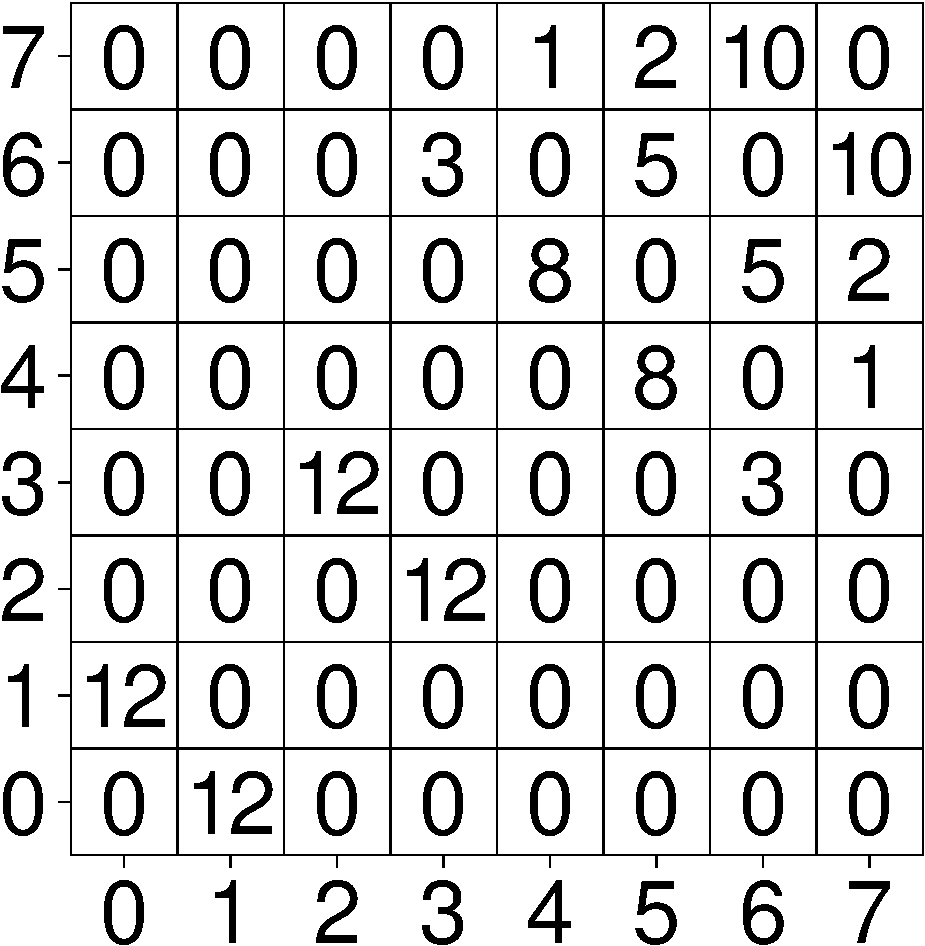
\includegraphics[width=0.3\textwidth]{figures/background/comm_matrix_num.pdf}
		\label{fig:comMatrNum}
	}
\hspace*{1cm}
	\subfigure[Colored matrix (heatmap).]{
		\label{fig:comMatrGraph}
		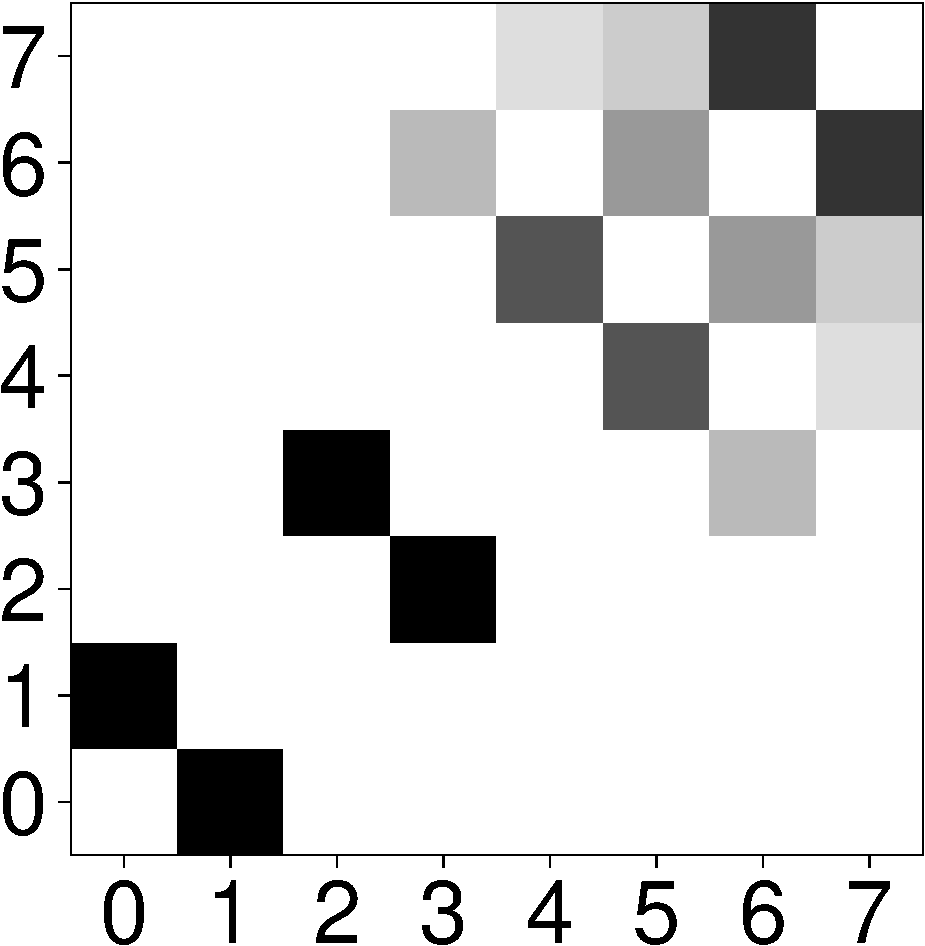
\includegraphics[width=0.3\textwidth]{figures/background/comm_matrix_graph.pdf}
	}
	\caption{Examples of communication matrices}
	\label{fig:comMatrExample}
\end{figure}
In \figurename~\ref{fig:comMatrGraph}, the matrix is represented graphically, where darker cells indicate more communication between pairs of threads~\cite{Diener:2016:2}.

\section{Improving STM applications with Thread Mapping}\label{sec:improvements}

To show how  sharing-aware thread mapping can improve the performance of an STM application, we designed an experiment that illustrates sharing-aware mapping of an STM application that calculates the sum of 16 million array elements. In the application, each group of 2 threads computes the sum of their respective array part in a shared sum variable. For example, with 8 threads, there are 4 shared variables for computing the sum.  The memory access behavior is known in advance: threads 0 and 1 access a shared variable, threads 2 and 3 another shared variable, and so on. Algorithm~\ref{alg:arraySumThread} shows how the sum function works. Lines \ref{alg:arraySumFirstLine}-\ref{alg:arraySumLastLine} verify the number
of the thread that is performing the sum and stores it in the respective shared variable. Thus, keeping threads that share a sum variable on sibling cores improves the cache usage. We used the \texttt{TinySTM}~\cite{TinySTM2} library for the synchronization of shared variables, with the default configuration: \emph{lazy} version management, \emph{eager} conflict detection and CM \emph{suicide}.

\begin{algorithm}[!tb]
	\caption{Function executed by each thread on the array sum application}\label{alg:arraySumThread}
	\small
	\begin{algorithmic}[1]
		\Function{sum}{}
		\Require
		\Statex \textbf{tid}: thread ID that is accessing this function
		\Statex
		\State \text{pinThreadToCore(tid, coreId)} \Comment{bind thread to core according to the strategy}
		\ForAll{value in array}
			\State	\text{stm\_start\_transaction()}   \Comment{begin transaction}
			\If{$(tid$ \text{in} $0,1)$}    \label{alg:arraySumFirstLine}
				\State \text{\textbf{stm\_write}(sum\_0\_1, \textbf{stm\_read}(sum\_0\_1) + \textbf{stm\_read}(value))}
			\ElsIf{$(tid$ \text{in} $2,3)$}
				\State \text{\textbf{stm\_write}(sum\_2\_3, \textbf{stm\_read}(sum\_2\_3) + \textbf{stm\_read}(value))}
			\ElsIf{$(tid$ \text{in} $4,5)$}
				\State \text{\textbf{stm\_write}(sum\_4\_5, \textbf{stm\_read}(sum\_4\_5) + \textbf{stm\_read}(value))}
			\ElsIf{$(tid$ \text{in} $6,7)$}
				\State \text{\textbf{stm\_write}(sum\_6\_7, \textbf{stm\_read}(sum\_6\_7) + \textbf{stm\_read}(value))} \label{alg:arraySumLastLine}
			\EndIf
			\State	\text{stm\_commit()}   \Comment{try to commit}
		\EndFor
		\EndFunction
	\end{algorithmic}
\end{algorithm}

We executed this application on the following NUMA machines: \textit{Xeon}, with 8 Intel E5-4650 processors, totaling 96 cores and 8 NUMA nodes and \textit{Opteron}, with 4 AMD Opteron 6276 processors, totaling 64 threads and also 8 NUMA nodes (more details on the machines in Section~\ref{sect:threadMapMethodology}). For the tests, 4 different configurations were used: the default ``Linux scheduler'', ``no cache sharing'', ``Cache sharing - Balance'' and ``Cache sharing - Socket''. With exception of ``Linux scheduler'', the mapping strategies are shown in \figurename~\ref{fig:MappingStrategyArraySum}.

\begin{figure}[ht]
	\centering
	\subfigure[No cache-sharing.]{
		\label{fig:MappingStrategyNoShare}
		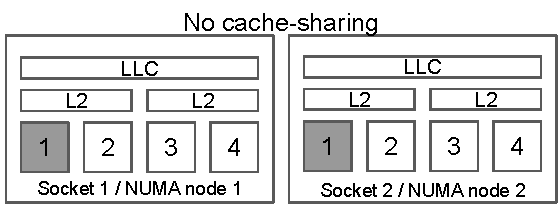
\includegraphics[width=0.48\textwidth,trim=0 0 0 17,clip]{figures/background/map-no-share.pdf}
	}%
	\subfigure[Cache sharing - Balance.]{
		\label{fig:MappingStrategyBalance}
		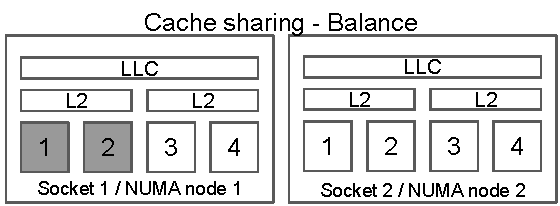
\includegraphics[width=0.48\textwidth,trim=0 0 0 17,clip]{figures/background/map-balance.pdf}
	}%
	\\
	\subfigure[Cache sharing - Socket.]{
		\label{fig:MappingStrategySocket}
		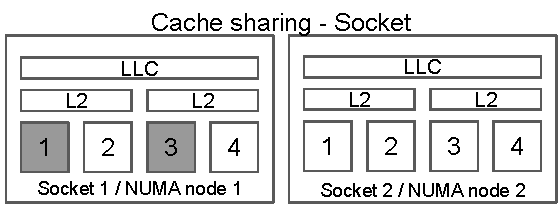
\includegraphics[width=0.48\textwidth,trim=0 0 0 17,clip]{figures/background/map-socket.pdf}
	}%
	\caption{Thread mapping strategies for the Array Sum application.}
	\label{fig:MappingStrategyArraySum}
\end{figure}

The idea of ``no cache sharing'' is to map threads that share the same variable to different NUMA nodes, forcing remote accesses and cache coherency messages between the nodes. In contrast, in the ``Cache sharing - Balance'' approach, the idea is to map threads that share a variable to sibling cores on the same NUMA node to share caches. However, for this configuration we map each pair of shared variables to different sockets.


Finally, for ``Cache sharing - Socket'', the idea is to place threads on sibling cores, sharing all cache levels. Since this application uses 8 threads, using this configuration all threads will be mapped to only one socket. To pin threads to cores the function \texttt{pthread\_setaffinity\_np} was utilized. The mapping was applied when a thread calls the function \texttt{stm\_init\_thread} of the \texttt{TinySTM} library. This function informs the STM runtime that the thread that has called it will perform transactional operations. \figurename~\ref{fig:arraySum} presents the execution time in seconds on each machine.


\begin{figure}[!ht]
	\centering
	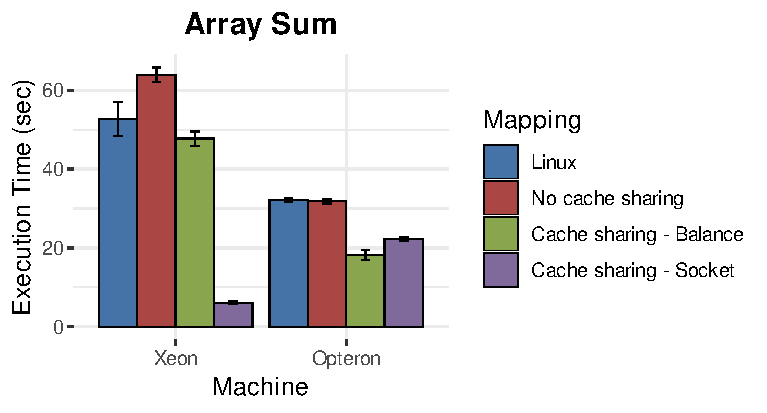
\includegraphics[width=0.7\textwidth]{figures/background/arraySum.pdf}
	\caption{Execution time of the Array Sum application.}
	\label{fig:arraySum}
\end{figure}


On the Opteron machine, the Linux scheduler had similar results as the ``no cache sharing''  configuration. When the application was running, we observed that the scheduler tries to balance threads, distributing them to the NUMA nodes, without taking the sharing behavior into account. This explains that the results are similar to ``no cache sharing''. On Xeon, the NUMA effects are more clear since forcing threads to run on distinct sockets, i.e., ``no cache sharing'' configuration, presented the worst performance.

%hurts the performance more than the Linux Scheduler.


For the ``Cache sharing - Balance'' configuration, on Xeon the execution time was reduced by 9.46\% whereas in Opteron it was reduced by 43.02\%. However, the most interesting result appears using ``Cache sharing - Socket'' mapping on the Xeon. Using this configuration, the execution time was reduced by 88.46\%. Although in Opteron the result of ``Socket'' was also positive (30.69\% of reduction time), the ``Balance'' configuration was better. We think that the good results of ``Socket'' on Xeon can be explained by the size of the last-level cache (LLC). The size of the data structures used by the array sum is 64MB. The size of LLC of the Xeon is 30MB whereas in Opteron it is 6MB. In that case, almost half of the memory used by the application fits entirely on the LLC of the Xeon. For the Opteron, mapping the variables to distinct cores increases the performance gains compared to ``Socket'' configuration, because more cache was available to the application.


\section{Summary}
This chapter presented the background related to this thesis. It also included a small experiment with a synthetic application to illustrate the possible benefits of sharing-aware thread mapping for STM applications.

\chapter{Related work}\label{chap:related}

This chapter presents the works related to the thesis subject. Section~\ref{sect:schedulers} describes transactional schedulers, one technique used to reduce the number of aborts during transactional execution, hence, improving the performance. Recent works use scheduling techniques for STM with the objective of optimizing resources, like cache and page sharing or to reduce the latency on data access. This kind of schedulers are described in Section~(\ref{sect:ThreadDataSTMRelated}), which presents an exhaustive list of works that uses thread and data mapping to improve the performance of STM applications. The next Section~(\ref{sect:ThreadDataRelated}) also describes works that explore thread and data mapping to improve the performance of applications that do not use STM. %However, those works are focused on general applications, not STM. 
To perform a successful mapping it is necessary to perform an in-depth analysis of STM applications, regarding sharing behavior. Hence, Section~\ref{sect:charactRelated} describes works that perform workload characterization of STM applications and sharing behavior of general applications.

\section{Transactional schedulers}\label{sect:schedulers}

Albeit a Contention Manager (CM) can help to reduce the number of aborts in a transactional execution, it has limitations. The CM acts only in a \textbf{reactive} way, dealing with a conflict when it occurs and not avoiding it \cite{Yoo:2008, Shrink, Nicacio:2012}. Transactional scheduling acts in a \textbf{proactive} way, using heuristics to prevent conflicts and to decide \emph{when} and \emph{where} a transaction should be executed \cite{Shrink}. %When the use of scheduling techniques on STM first appeared, the main idea was to avoid conflicts, and the solution, in general, was serializing a conflicting transaction. Recent works use schedulers for STM with the objective of optimizing resources, like cache and page sharing or to reduce the latency on the data access.

This section presents state-of-the-art transactional scheduling techniques. In order to identify the works on this subject, the surveys \cite{Hendler:2015} and \cite{Sanzo:2017} were used as a basis. Also, this section describe works published after the surveys. However, transactional schedulers focused on HTM, GPU (Graphics Processing Unit) or real-time systems are not included, because they are not on the scope of this thesis. Di Sanzo~\citeyearpar{Sanzo:2017} classifies the schedulers as reactive, prediction-driven, feedback-driven (all heuristic based) and machine learning or analytical (based on performance models \cite{Tay:2018}). In the next sections, we will follow this classification to describe the transactional schedulers.

\subsection{Feedback-driven}\label{sec:feedback}

Feedback techniques are based on constantly comparing if the \emph{actual behavior} of a system is the \emph{desired} \cite{Janert:2013}. Application parameters are monitored during the execution of a transaction (\emph{actual behavior}), and in each new iteration, they are used as input for the scheduler to take decisions, i.e., a corrective action in order to achieve the \emph{desired behavior}. This step is repeated during execution, trying to dynamically adjust the application \cite{Sanzo:2017}.

One of the first works to propose a transaction scheduler for  STM was the \textit{Adaptive transaction scheduling} (ATS)~\cite{Yoo:2008}, and the idea was to work together with the CM: each thread has a \emph{contention intensity} (CI), recalculated each time that a transaction finishes (commit or abort). When the CI is great than a predefined threshold, threads are inserted in a global queue to be serialized. This approach takes into consideration that when the CI is high, it is better to limit parallelism, avoiding possible conflicts. 

In \citeNamesYearPar{Ansari:2008_1}, an adaptive concurrency control (ACC) technique was proposed which limits the maximum number of concurrent threads executing transactions. The idea is that an excessive number of threads can hurt the performance in a high contention environment, mainly due to a higher number of aborts. The technique keeps track of a \emph{Transaction Commit Ratio} (TCR), i.e., the percentage of committed transactions in the total number of transactions executed, and uses it to dynamically adapt the number of concurrent threads. The ACC uses two parameters: a \emph{target TCR range} and a time \emph{interval} for calculating the TCR. Four adaptive concurrency control algorithms were proposed, varying the heuristic to change the total number of active threads, but all based on TCR. 

In \citeNamesYearPar{Ansari:2008}, the authors proposed a new concurrency control algorithm, called \emph{P-only Concurrency Controller} (\texttt{PoCC}), extending the ACC work. The main idea is to keep TCR at a configurable value (called \emph{set point}) instead of a range as in the previous work. If a high \emph{set point} is chosen, then the number of threads will quickly reduce when TCR decreases. On the other hand, it will have a slower response when TCR grows suddenly. 

\citeNamesYearPar{Chan:2011} also propose a new concurrency control technique. For this purpose, a parameter \emph{quota} is recalculated every predetermined amount of time. When a new transaction is to be started, it needs to check if there is sufficient quota available, otherwise, it will wait. There are two proposals for calculating the \emph{quota}. The first one, called \emph{Throttle}, adjusts the quota based on the commit \emph{ratio}, which is compared with a predefined threshold, and the quota is adjusted according to it. The second one, called \emph{Probe}, uses commit \emph{rate} (total of commits per unit of time) instead of \emph{ratio}. Also, it uses a try and error approach to find the best quota, instead of a fixed threshold. 

\citeNamesYearPar{Ansari:2014} published another work using TCR as the main heuristic. The difference from their first work \cite{Ansari:2008_1} and \texttt{PoCC} is that in this new algorithm, called \emph{Weighted Adaptive Concurrency Control} (\texttt{WACC}), the TCR is calculated per thread. Similar to \texttt{PoCC}, that tried to keep TCR at a configurable value (\emph{set point}), \texttt{WACC} uses the notion of \emph{expected TCR}. It predicts the global TCR that should be achieved if the determined subset of threads is activated. Thus, it is possible to predict if the \emph{set point} will be reached if the determined subset of threads will be allowed to concurrently run. Like in the first work \cite{Ansari:2008_1}, four approaches are proposed, using different heuristics (all based on TCR) to define the total number of threads. 

One of the main objectives of \citeNamesYearPar{Rito:2014}, is to avoid excessive serialization using a fine-grained approach. They have proposed the \texttt{ProPS} (\emph{Progressively Pessimistic Scheduling}) technique. In \texttt{ProPS}, a global \emph{concurrency level} ($CL$) matrix  keeps information about pairs of atomic operations $i$ and $j$. For the authors, each transaction that executes the same block of code, execute the same operation of type $i$. Accessing the matrix on the index $CL_{ij}$, it is possible to know how many transactions executing atomic operations of type $i$ could be executed concurrently with another one executing $j$ atomic operations. In the beginning, the values in the matrix are set to be equal to the maximum of threads or cores of the machine, i.e., all cores could execute all types of transactions without restriction. When a specific $CL_{ij}$ decreases (typically by an abort of $i$ or $j$), \texttt{ProPS} reduces the number of transactions executing $i$ and $j$. By design, \texttt{ProPS} reduces exponentially (\emph{progressively pessimistic}) the concurrency on aborts between atomic operations and increases it linearly at commit. 

The idea proposed by \citeNamesYearPar{Pereira:2014} is to use the \emph{percentage of effective work} (\texttt{PEW}) of a transaction as the main heuristic. The \texttt{PEW} replaces CI in approaches like \texttt{ATS}. It is calculated for each transaction, and it is based on the total of cycles executed until the transaction finishes (commit or abort). Transactions with less effective work done are prioritized. If a transaction aborts and the \texttt{PEW} is high, then it is wasting too many work (cycles) and should have a lower priority. There are queues of transactions according to their priorities. The authors noted that only using \texttt{PEW}, there is still a high number of conflicts between transactions with the same priority. Thus, an additional heuristic was included: a \emph{success-reward policy} (SRP). According to a predefined \emph{reward} threshold, a transaction could change its position in the queue. 

In \citeNamesYearPar{Ravichandran:2014}, the authors classified applications as  \emph{fully scalable} and \emph{scalability limited}. Applications under the former classification decrease their execution time as the number of cores of the machine grows. The latter is the opposite, hurting the application performance as the number of cores is increased. The authors have proposed \texttt{F2C2-STM} (Flux-based Feedback-driven Concurrency Control), which focuses on \emph{scalability limited} applications. \texttt{F2C2-STM} is inspired by TCP’s (Transmission Control Protocol) network congestion control algorithm, to adjust the maximum number of concurrent threads allowed to run. The heuristic utilized is the transaction throughput. However, to compute the global throughput between all threads, a global variable is needed. To avoid synchronization, the authors chose to calculate the throughput only in one thread. Thus, they have assumed that the transactional workload is roughly the same between all threads. To find the best concurrency level, like in \citeNamesYearPar{Chan:2011}, they have used a try and error approach, monitoring the transaction throughput on each modification. 

\subsection{Reactive}\label{sec:reactive}

Reactive techniques are activated after a conflict is detected. The main objective is to avoid the same conflict to occur again~\cite{Sanzo:2017}.

The \emph{Collision Avoidance and Resolution} (\texttt{CAR-STM}) scheduling-based mechanism \cite{Dolev:2008} presents two new CMs and a scheduler. Each core has one queue, and the runtime system restricts the maximum number of threads to be equals to the cores available. The first CM proposed is called \emph{Basic}. When it detects a conflict between two transactions, it aborts the newer transaction and move it to the queue of the older. The second, called \emph{Permanent}, also aborts the newer transaction in case of conflicts. However, it marks the aborted as a subordinate of the older. If a transaction needs to be moved to another queue, \emph{Permanent} will also move all its subordinates. A proactive centralized module tries to choose the queue for a new transaction, based on a conflict probability with the running transactions on each queue. 

On Steal-on-Abort (\texttt{SoA}) \cite{Ansari:2009}, the idea is to find dynamically an optimal order to execute transactions, minimizing aborts. Each thread has two queues. The first one, called main queue, keeps new transactions that should be processed by the thread. The second queue is called ``steal''. When a transaction aborts due to a conflict, instead of restarting immediately, the opponent transaction ``steals'' the aborted one and put in the steal queue of the thread. When the opponent transaction commits, transactions on the steal queue are moved to the main queue. The authors proposed different strategies to choose in what position of the queue the stolen transaction will be put in. According to the authors, \texttt{SoA} benefits applications that have a high number of repeated conflicts. 

In Attiya and Milani~\citeyearpar{Attiya:2009,Attiya:2012}, the focus of the proposed schedulers are workloads with read-dominated transactions and lazy versioning. The authors explain that many proposed schedulers focuses on avoiding repeated conflicts, serializing transactions. Also, they do not perform well under read-dominated workloads, serializing more transactions than necessary. With this motivation, the \texttt{BIMODAL} scheduler is proposed. On \texttt{BIMODAL}, each core has a work queue. Also, a global \emph{RO-queue}, for read-only transactions is shared between all cores. When two transactions conflict, if the aborted is a writing one, it will be moved to the same queue of the conflicting. If it is read-only, it will be moved to the RO-queue. When the RO-queue reaches a threshold of enqueued transactions  (or the other queues are empty), the \texttt{BIMODAL} will prioritize the transactions in the RO-queue. The scheduler is proposed in a theoretical way. It was formally proved and compared with \texttt{SoA}.

\citeNamesYearPar{Sharp:2013} argue that prior transactional schedulers deal with concurrent conflicts only, i.e., between a reader and a writer. The objective of the authors is to deal with \emph{semantic conflicts}. This kind of conflict occurs when there is no concurrent conflict and yet it is not possible for transactions to proceed. They have cited as an example a transaction that needs to consume an item from a buffer but the buffer is empty, or a withdraw in an account without funds. With this motivation the \texttt{Hugh} scheduler is proposed. When a transaction aborts, it first needs to register itself in a \emph{transaction table}. Next, a speculative phase begins, executing a permutation of transactions that is in the \emph{transaction table}. This phase tries to find a permutation where the maximum of pending transactions can commit. Finally, in the commit phase, all successful permutations are sent to an algorithm to decide which permutation can commit. It chooses the permutation with the greatest number of transactions. The authors also proposed \texttt{Hugh2}~\cite{Sharp:2014}, using the same idea on a different STM implementation.

The \emph{second-hop conflict} is a concept proposed in the \texttt{RelSTM} scheduler \cite{Sainz:2013}. If a transaction $T_{1h}$ conflicted with $T_x$, and another $T_{2h}$ has conflicted with $T_{1h}$, then $T_{2h}$ is a \emph{second-hop} of $T_{1h}$. Upon a conflict, the transaction registers its opponent and those that have conflicted with the opponent too. When restarting, the transaction is serialized if the opponents are still running. Otherwise it could wait if a percentage of \emph{second-hop} transactions that are still running is greater than a predetermined threshold. 

\subsection{Prediction-driven}\label{sec:prediction}

Schedulers under this classification, use prediction techniques, trying to increase the probability to make the right decision on  scheduling \cite{Sanzo:2017}.

The \texttt{Shrink} scheduler \cite{Shrink} tries to predict the future memory accesses of transactions based on past accesses. The authors use the concept of temporal locality of the read-set. They have identified that multiple consecutive committed transactions in a thread access similar addresses. A per thread \textit{Bloom Filter}\footnote{\textit{Bloom Filter} is a probabilistic data structure which allows fast search and insertion of data \cite{Bloom:1970}.} keeps track of the last read addresses. When an address is read, \texttt{Shrink} verifies if it is in the \textit{Bloom Filter}. If true, it was recently accessed and it is included in the \emph{predicted read-set} of the thread. In case of abort, the write-set is copied to the \emph{predicted write-set}. Each thread has a \emph{commit rate}, calculated every time that a transaction commits or aborts. When the commit rate is greater than a predefined threshold, \texttt{Shrink} verifies, before starting a transaction, if some address in the prediction sets (read or write) are being written by other threads. If true, the serialization is activated. 

In \citeauthoronline{Heber:2012}~\citeyearpar{Heber:2009,Heber:2012}, the focus is to avoid too much oscillation between serialization and non-serialization periods. The authors proposed a mechanism called \emph{Low-Overhead Serializing} algorithm (LO-SER) which aims to keep certain stability between serialization times. The scheduler collects statistics like past commits and aborts. This data can be local (per thread) or global. The proposed stabilizing mechanism calculates a \emph{contention level} (CL) each time that a transaction aborts or commits. Then, a low ($lt$) and a high threshold ($ht$) needs to be defined, i.e., a range. Serialization is applied if CL is greater than $ht$ and deactivated when CL is lower than $lt$. 

\citeNamesYearPar{Atoofian:2011} uses the intuition that if a transaction aborted, it will fail again in the future. This theory is called \emph{locality of contention}. To avoid it, it is important that the transaction that caused the abort should finish before restarting the aborted. With this motivation, the \emph{Speculative Contention Avoidance} (\texttt{SCA}) mechanism is proposed. Each thread has a Contention Predictor (CP), composed by a \emph{contention bit} (CB) and a \emph{saturating counter} (SC). The CB shows the result of the last transaction executed on the thread (1 if failed or 0 if committed). The SC is similar to branch predictors used in pipelines processors \cite{Yeh:1992}. It is incremented each time that a transaction conflicts and zeroed when commits. Before a thread executes, it consults the \texttt{SCA}, that will serialize the transaction if CB is equals to 1 and SC is greater than a given threshold. 


\subsection{Mixed Heuristics}\label{sec:mixedHeuristic}
This section describes works that use mixed strategies according to different transaction profiles. For instance, a transaction initially uses a lightweight feedback-driven technique. However, if the size of a transaction (for instance, based on the amount of memory locations read) is above a given threshold, the system switches to a more complex heuristic.

In \citeauthoronline{Nicacio:2011}~\citeyearpar{Nicacio:2011,Nicacio:2012}, the \emph{Light-Weight User-Level Transaction Scheduler} (\texttt{LUTS}) is proposed. In \texttt{LUTS}, each transaction that executes the same critical section shares an identifier (ID). The main idea is to have different scheduling heuristics according to  transaction length. The number of cycles  is utilized to define if a transaction is long or short. If it is considered short, the heuristic used is similar to \texttt{ATS}, using a contention intensity (CI). The difference is that the CI is calculated per transaction ID, instead of per thread like in the original \texttt{ATS}. Moreover, if a transaction is serialized, \texttt{LUTS} tries to choose one with different ID to replace it. If a transaction is considered long, a more sophisticated (and expensive) heuristic that uses additional data structures is utilized, trying to predict and avoid conflicts. The system uses a fixed thread that is responsible for calculating the length of transactions. Another feature, like in \texttt{CAR-STM}, is to restrict the maximum number of threads to be equal to the cores available.

An extension for \texttt{LUTS} was proposed in \cite{Pereira:2013}, called \texttt{BAT} (\emph{Best Alternative Transaction}). In \texttt{LUTS}, the CI is utilized for short transactions only. \texttt{BAT} utilize the CI for long transactions too, as an additional parameter for helping to choose the best transaction to be scheduled. In other words, CI is calculated for all transactions. For short ones, it is the unique parameter used to decide which transaction is allowed to run, i.e., with less probability of conflicts. For long transactions, there are more data structures used together with CI to decide it. 

The \texttt{ProVIT} scheduler \cite{Rito:2015} uses the same idea from \texttt{LUTS}, where there are distinct heuristics according to transaction lengths. However, in \texttt{ProVIT} it is possible to have two heuristics active at the same time, i.e., each thread using a different heuristic. A transaction is considered long if the size of their read-set is greater than a predefined threshold. This information is updated dynamically and, on start, transactions are considered short. For short transactions, the heuristic is based on the previous work of the authors, \texttt{ProPS}, described in Section \ref{sec:feedback}. When a transaction aborts, the read-set is verified to check if it is a long transaction. If true, it is marked as a VIT (\emph{Very Important Transaction}) and its read-set is copied to a data structure available for all threads. Before a writing transaction commits, it needs to check if its write-set has any intersection with the read-set of any VIT transaction. If it has, the commit should be delayed, giving priority to the VIT. The idea is to avoid a VIT to abort again. 

\subsection{Others}\label{sec:otherSchedule}

This Section describes works that use machine learning (ML), analytical performance models of  applications or other techniques. As these techniques are out of scope of this thesis, they will not be described in details.

Extending the Linux Kernel for supporting STM scheduling was explored in \citeauthoronline{Maldonado:2011}~\citeyearpar{Maldonado:2010,Maldonado:2011}.

The idea of using ML and analytical models in schedulers was widely explored by Rughetti and Sanzo. Controlling the total of threads allowed to concurrently run was proposed in \texttt{SAC-STM} \cite{Rughetti:2012}, using neural networks, and in \texttt{CSR-STM} \cite{Sanzo:2013} with analytical performance models. Also, in \citeNamesYearPar{Rughetti:2014} a work integrating \texttt{SAC-STM} and \texttt{CSR-STM}, named \texttt{AML} was proposed. Later, \citeNamesYearPar{Rughetti:2014_2} describe an extension to \texttt{SAC-STM}, called \texttt{DSF-STM}. In Di Sanzo et al.~\citeyearpar{Sanzo:2016,Sanzo:2020}, a Markov chain-based analytical performance model is proposed to dynamically control the total of concurrent threads executing transactions allowed to run. \citeauthoronline{Castro:2011}~\citeyearpar{Castro:2011,Castro:2012} have used ML techniques to choose  the best \emph{thread mapping} for improving  STM performance. \citeNamesYearPar{Popovic:2017} and \citeNamesYearPar{Popovic:2019}, proposed schedulers for Python-STM~\cite{PythonSTM}, using ML techniques.

Finally, \citeNamesYearPar{Marques:2016}, have proposed \emph{Dynamic Serializer} (DS). Different from prior approaches, they have focused on reducing energy consumption instead of performance.

\section{Thread and data mapping in STM}\label{sect:ThreadDataSTMRelated}

The works studied so far use transactional scheduling to avoid conflicts between transactions. This section describes works which aim to use scheduler techniques on STM focusing on optimizing resources. For example, trying to keep threads on sibling cores to share caches or load balance in multiprocessor systems.

\citeNamesYearPar{Castro:2014} have studied how \emph{thread mapping} could be utilized for improving STM performance. First of all, they describe four different possible thread mappings that could be utilized: Scatter, Compact, Round-Robin and Linux. The proposed mechanism dynamically collects information to decide the mappings. The first strategy was called \emph{Conflict}. It uses the \emph{abort ratio} (AR) as the main heuristic. The intuition utilized is: if AR is high (based on a threshold), the application is accessing a great quantity of shared data. In these cases, using a \emph{Compact} mapping could be useful for sharing caches. If AR is moderated, \emph{Round-Robin}, the intermediate solution, is used; otherwise \emph{Scatter}. The second strategy is called \emph{Test}. It uses the three mappings on a fixed period of time and computes the execution time of each of them. At the end, the mapping that had the minor execution time is selected. 

In \citeNamesYearPar{Chan:2015} a thread mapping mechanism called \emph{Affinity-Aware Thread Migration} is proposed. It aims to detect threads that access common data, keeping them in sibling cores on the same processor to share caches. To compute which threads are sharing data, they have used a matrix $n \times n$, where $n$ is the maximum of threads that the system supports. When a thread $i$ conflicts with a $j$, i.e., aborts, the respective index $i,j$ is updated in the matrix, using the CI (contention intensity) proposed in \texttt{ATS} (Section \ref{sec:feedback}). The intuition used is: if two threads conflict, they were accessing the same shared data. This matrix represents a graph, with edges and their weights. The objective is to reduce the sum of edges between processors. Only a pair is migrated per time. 

In \citeNamesYearPar{Zhou:2018} a concurrency control mechanism to dynamically adjust the total number of active threads executing transactions is proposed. Also, as the total of threads changes, the authors also adjust thread mapping. The mappings utilized are the same from \citeNamesYearPar{Castro:2014}, i.e, \emph{Scatter}, \emph{Compact}, \emph{Round-Robin} and \emph{Linux}. The heuristic for deciding the total number of active threads is based on \emph{commit ratio}~(CR) and \emph{throughput}. In the beginning, two or more threads (configurable) are allowed to run concurrently. Each period of time, the CR and the throughout are computed, adjusting the total of threads according to it. For thread mapping, the STM system is initialized with the \emph{Linux} default mapping, and after a certain time, it changes to \emph{Round-Robin} (intermediate solution). If the throughput is higher, then \emph{Compact} is used. If performance decreases, then \emph{Scatter} is used. 

\citeNamesYearPar{Goes:2014} focused on STM applications that have a worklist pattern, i.e., they have a single operation responsible to process an item of work from a dynamically managed worklist. Regarding \texttt{STAMP} benchmark, four applications present this pattern: \emph{intruder}, \emph{kmeans}, \emph{vacation}, and \emph{yada}. The idea is encapsulated STM application as a skeleton framework, improving the memory affinity by using static page allocation (bind or cyclic) and data prefetching by using helper threads. Helper threads make use of idle cores to bring potentially useful data for the LLC. The memory affinity mechanism is called \texttt{SkelAff} and it was implemented inside a proposed \texttt{OpenSkel} framework. Hence, STM applications need to be rewritten with this framework to be able to use the memory affinity improvements. It is worth noting this proposed framework is only able to deal with one specific kind of sharing pattern.

\section{Thread and data mapping in general applications}\label{sect:ThreadDataRelated}

This section presents works that use thread and/or data mapping to improve data locality of applications that do not use STM, running on shared memory architectures. To identify the works on this subject, the surveys \cite{Diener:2016Sur} and \cite{Cruz:2018} were used as a basis. We exclude two works described in the papers, because they were out of scope: compiler analysis and fixed runtime options. The former relies on complex analysis that will modify the entire application and not only the STM implementation. Also, this technique usually is limited to specific compiler versions \cite{Diener:2016Sur}. The latter is used to specify global and static policies, that will be kept fixed until the application finishes, such as interleave for data or round-robin for thread mapping. The remaining  techniques will be grouped into two groups: offline and online techniques. Finally, works that focuses on distributed memory, like \emph{Message Passing Interface} (MPI) will not be included, as this thesis does not focus on STM for distributed systems. Although MPI can be used for shared memory architectures, the form of communication is explicit, i.e, tracking the sent messages is possible to discover threads the are communicating often~\cite{Cruz:2018}.

\subsection{Offline Techniques}\label{sect:offlineTec}

This kind of technique consists of analyzing the source code of the application or profiling and executing it, to identify the memory access behavior \cite{Diener:2016Sur}. 
Then, the application is modified, either manually or automatically, applying an improved mapping.  Behavior analysis happens before execution. At run time, no profile information needs to be collected. However, if the application changes its behavior dynamically, the profile phase will fail on getting precise information about memory access \cite{Diener:2016Sur}. Profiling could be implemented manually, using system call functions or with the help of instrumentation tools like \texttt{Pin} \cite{Luk:2005}.

Regarding manually analyzing and source code modifications, some tools could help programmers in this task. \texttt{libnuma} \cite{libnuma} is a library and command-line tool that is a wrapper for kernel system calls to set memory policies on NUMA architectures. Using \texttt{libnuma} as a library, it is possible to allocate memory on a specific NUMA node and the policy to be used, like interleave. Also, it is possible to bind a thread to run on the CPUs of a specific NUMA node. Ribeiro et al. \citeyearpar{Ribeiro:2009,Ribeiro:2011} have proposed the tools \texttt{MAi} (Memory Affinity interface) and \texttt{Minas}. \texttt{MAi} is a user-level interface focused on numerical scientific HPC applications. It provides optimizations for arrays and memory policies to manage data allocation. The main optimization was made on arrays. When using \texttt{MAi} to allocate memory for an array, the programmer can specify the data distribution, i.e., how rows and columns should be distributed in the NUMA nodes. Also, \texttt{MAi} implements thread scheduling to ensure data locality. \texttt{Minas} is a portable framework for managing memory affinities explicitly or automatically on NUMA architectures. \texttt{Minas} has a preprocessor to perform automatic source code modifications and optimizations analyzing the NUMA architecture where the application is compiled. For manual controlling of the memory affinity in the source code, \texttt{Minas} uses \texttt{MAi}. Another library is \texttt{TBB-NUMA} \cite{Majo:2015, Majo:2017}, that is an extension of the Intel Threading Building Blocks (TBB) \cite{Reinders:2007}. It includes functionalities for manual management of data allocation between NUMA nodes, automatic thread mapping and other features to make the library NUMA-aware. 

Two works use the described tools to achieve better thread and data affinity. \citeNamesYearPar{Dupros:2010} have studied the impact of memory affinity in seismic simulations. After a detailed study of the source code and the underlying NUMA architecture where the application was executed, \texttt{MAi} was utilized for efficient thread and data mapping of the application. \citeNamesYearPar{Cruz:2011} made similar studies on the NAS Parallel Benchmark (NPB) \cite{NPB:1999}, and after the detailed analysis of the applications, they have used \texttt{Minas} for applying the improved thread and data mapping.

There are works that first execute an application to get detailed information about the memory access pattern. Then, this information is used to improve performance. \citeNamesYearPar{Diener:2010} recorded in a communication matrix which threads have accessed the same memory location. After that, an algorithm uses this matrix to find the best placement of the threads. If a machine support 16 threads at maximum, then it is feasible to do an exhaustive search, i.e., trying every possible placement. Otherwise, an heuristic is applied. \citeNamesYearPar{Majo:2012} have studied the access pattern of scientific benchmarks. The applications were profiled using hardware counters of the Intel Nehalem processor. Also, the source code of the applications were studied in detail, to identify the access patterns of matrices, a common data structure on scientific computation. With this information, the authors have proposed new primitives to be used in OpenMP, to have better control on data distribution and  loop iterations over the data structures. \citeNamesYearPar{Mariano:2016} have made a detailed study in the source code of the HashSieve algorithm, which is used in the context of the lattice-based cryptography technique~\cite{Micciancio:2009}. The optimization was made by reordering some operations to leverage cache locality, prefetching data and changing data structures used in the algorithm. \citeNamesYearPar{Denoyelle:2019} have created ML models to choose the best placement of threads and data of applications. They have used different types of thread placement (compact and scatter), data policies (first-touch and interleave) totaling 4 combinations. The application is executed using a default configuration (compact and first-touch) and a set of metrics are collected using instrumentation and hardware counters. Hence, these metrics are processed and used as an input parameter to mathematical and machine learning models. These trained models can identify the best placement for the applications.

Analyzing tools were proposed to collect information about  memory access of  applications. These tools help to understand how applications share data. \texttt{Numalize} \cite{Diener2015} is based on the Pin instrumentation tool \cite{Luk:2005}. The authors also proposed metrics to characterize communication and page usage of applications. Thus, \texttt{Numalize} generates a memory trace of applications and calculates the proposed metrics. The generated information helps to choose the best placement of threads and data. \texttt{TABARNAC}~\cite{Beniamine:2015} is similar to \texttt{Numalize} and provides graphical visualization of memory access behavior, like the distribution of the accesses by threads and data structures. A most recent tool, \texttt{NumaMMa} (NUMA MeMory Analyzer) \cite{Trahay:2018} uses hardware counters of a processor to generate memory traces. When the application finishes, \texttt{NumaMMa} processes the trace and analyzes the cost of memory accesses of each object and how threads access them. Also, graphical visualization of the processed information is available.

\citeNamesYearPar{Denoyelle:2019}, obtain information about the characteristics of applications through a preliminary execution. This information is collected using instrumentation or hardware performance counters. After that, using machine learning, the collected information is processed and, resulting in information if application is sensitive to locality and the best thread and data placement. Then, the application is re-executed using the proposed placement.


\subsection{Online Techniques}\label{sect:onlineTec}

Online techniques collect information about  memory access during the execution of the application and perform  mappings dynamically. The main advantage is that no prior execution is needed to collect information. However, the main challenge is to create an heuristic that takes into consideration the trade-off between accuracy and runtime overhead \cite{Diener:2016Sur}. Analyzing all memory accesses of an application is the best strategy for deciding mappings, but the overhead added makes it unfeasible \cite{Cruz:2018}. Thus, usually, the methods used to collect information about memory accesses is based on sampling. Also, the migration of threads and  pages represent an overhead that should be considered.

\citeNamesYearPar{Ogasawara:2009} have used the Garbage Collector (GC) of the Java programming language to identify the preferred NUMA node for objects. During the collection phase, the proposed method determines which threads have most accessed certain objects, i.e., the \emph{Dominant Thread} (DoT). Then, the GC migrates the objects to the NUMA nodes where the DoT is running.

\texttt{ForestGOMP} \cite{Broquedis:2010} is an extension of OpenMP that uses hints provided by application programmers, compiler techniques and hardware counters to perform dynamically thread and memory placement. It uses internally libraries like \texttt{hwloc} to compute the underlying hardware hierarchy and the \texttt{BubbleScheduler} framework \cite{Thibault:2007}. Threads that share data or synchronize often are organized in bubbles. The main objective of the proposed scheduler used by \texttt{ForestGOMP} is to improve the cache usage by making each ``bubble'' access the local memory, migrating pages if necessary. The scheduling actions are triggered when resources are (de)allocated, a processor becomes idle or a hardware counter exceeds a predefined threshold.

\texttt{autopin} \cite{Klug:2011} is a framework that extends the \texttt{pfmon} utility from the \texttt{perfmon2} package \cite{Eranian:2005}. \texttt{pfmon} is a command line tool that accesses hardware performance counters of processors. Through an environment variable it is possible to choose a set of mappings, i.e., the cores to be used and the order that they should be assigned to threads. A command-line parameter is available for setting a hardware counter that \texttt{autopin} should use for calculating the performance rate. After the initialization, if more than one set of mappings was defined, \texttt{autopin} will test each one, calculating the performance based on the timestamp and the hardware counter chosen. After all mappings have been tested, the one which achieves the best performance will be chosen and will be active until the application finishes. 

The focus of the \texttt{BlackBox} scheduler \cite{Radojkovic:2013} is applications with a low number of threads and many instances, like networking applications. It tries to test all possible thread mappings (assignments) and chooses the one that achieves the best performance. It has 3 distinct phases. The first one profiles the target application. The main information collected are conflicts and shared resources, like caches and memory controllers. The second phase uses the information collected to predict the performance of a determined thread assignment. If the number of threads and instances are low, all possibilities are tested. Otherwise, only 1000 combinations are evaluated. The last phase chooses the best 5 predicted models and tests them to make sure that the best one was chosen.

\citeNamesYearPar{Tam:2007} have used hardware performance counters of the IBM Power5 processor to track cache misses between chips, i.e., if the miss was local or remote. Each thread has a data structure to keep track of data regions accessed that caused a remote cache miss. This information is retrieved from a counter in the processor. Analyzing all cache misses would be unfeasible, thus, the authors sampled the monitoring. The next step is to analyze data structures looking for data sharing between threads. If found, threads are mapped to the same chip, for sharing caches. After that, the monitoring phase starts again. The proposed scheduler was tested with a synthetic micro-benchmark and three commercial server workloads. In \citeNamesYearPar{Azimi:2009} the authors have extended the studies of how the hardware performance counters could be utilized for improving locality of threads. They have presented the usability and importance of hardware performance counters as a low-overhead resource to get accurate online information about performance.

Regarding data mapping, \citeNamesYearPar{Lof:2005} have studied how a next-touch directive could improve the performance of industrial applications. 
One application was chosen that uses a large matrix initialized by the main thread. After the initialization, it consumes about 500 MB of memory. Using the default Linux OS data mapping, first-touch, all pages will be allocated in the first node. With next-touch, the data will be migrated according to the accesses of threads. The author has identified a great overhead on page migrations, due to TLB (translation look-aside buffer) shootdowns, i.e., the mechanism that keeps the TLB's coherent \cite{Villavieja:2011}. To overcome this limitation, they have proposed to use larger pages, e.g., 64Kb instead of 8Kb.

The \emph{Communication Detection in Shared Memory} (CDSM)~\cite{cdsm} is a Linux kernel module to detect communication patterns of parallel applications and migrate threads according to their memory affinity. It keeps track of page faults to detect the communication between threads. The \emph{kernel Memory Affinity Framework} (kMAF)~\cite{kmaf} is implemented directly in the Linux kernel, extending the idea of CDSM to the problem of data mapping in NUMA architectures. The \emph{Carrefour} mechanism~\cite{Dashti:2013} is also implemented directly in the Linux kernel. However, it uses Instruction-Based Sampling (IBS) available only in AMD processors. \citeNamesYearPar{Barrera:2020} have the same objective of \citeNamesYearPar{Denoyelle:2019} (described in Section~\ref{sect:offlineTec}), however their model works online, and they have added prefetching optimizations beyond thread and data placement.


%\texttt{ForestGOMP}~\cite{Broquedis:2010} is an extension of the OpenMP runtime that uses hints provided by programmers, compiler techniques, and hardware counters to perform dynamically thread and memory placement. Threads that share data or synchronize often are organized in bubbles. The main objective of the proposed scheduler used by \texttt{ForestGOMP} is to improve the cache usage and try to make each ``bubble'' access local memory, migrating pages if necessary. The focus of the \texttt{BlackBox} scheduler~\cite{Radojkovic:2013} is applications with a low number of threads and many instances, like networking applications. It tries to test all possible thread mappings and chooses the one that achieves the best performance. If the number of threads and instances are low, all possibilities are tested. Otherwise, only 1000 combinations are evaluated.

%The \emph{Communication Detection in Shared Memory} (CDSM)~\cite{cdsm} is a Linux kernel module to detect communication patterns of parallel applications and migrate threads according to their memory affinity. It keeps track of page faults to detect the communication between threads. The \emph{kernel Memory Affinity Framework} (kMAF)~\cite{kmaf} is implemented directly in the Linux kernel, extending the idea of CDSM to the problem of data mapping in NUMA architectures. The \emph{Carrefour} mechanism~\cite{Dashti:2013} is also implemented directly in the Linux kernel. However, it uses Instruction-Based Sampling (IBS) available only in AMD processors.

%Some works first execute an application to get detailed information about the memory access pattern (profiling). Then, the application is re-executed, using the collected information to improve performance. Diener et al. \cite{Diener:2010} recorded in a communication matrix which threads have accessed the same memory location. After that, an algorithm uses this matrix to find the best placement of the threads to cores.
%\citeNamesYearPar{Majo:2012} have studied the access pattern of scientific benchmarks. The applications were profiled using hardware counters. Also, the source code of the applications were studied in detail, to identify the access patterns of matrices, a common data structures on scientific computation.
%With the collected information the authors have proposed new primitives to be used in OpenMP, to have better control on data distribution and loop iterations over data structures. \citeNamesYearPar{Mariano:2016} have made a detailed study in the source code of the HashSieve algorithm, which is used in the context of the lattice-based cryptography technique~\cite{Micciancio:2009}.
%The optimization was made by reordering some operations to leverage cache locality, prefetching data and changing data structures used in the algorithm. \citeNamesYearPar{Denoyelle:2019}, obtain information about the characteristics of the applications through a preliminary execution. This information is collected using instrumentation or hardware performance counters. After that, using machine learning, the collected information is processed and, resulting in information if application is sensitive to locality and the best thread and data placement. Then, the application is re-executed using the proposed placement. \citeNamesYearPar{Barrera:2020} have similar goals, however their model works online, i.e., during runtime and they added prefetching optimizations beyond thread and data placement.

\section{Workload characterization}\label{sect:charactRelated}

In \citeNamesYearPar{Williams:2009}, the Splash-2 and Parsec benchmark suites were characterized regarding their memory access behavior. They also showed other characteristics such as temporal and spatial characterization of the communication. All information was gathered through the use of a simulator. Using the collected information, they proposed changes to the communication systems to be used in future chip multiprocessors (CMP). Different communication characteristics of Splash-2 and Parsec were also studied in \cite{Mohammed:2015}. \citeNamesYearPar{Rane:2011} proposed to instrument the source code of applications using the LLVM compiler, to extract memory trace of applications. Then, they compute metrics using the collected data, such as cycles per access; NUMA hit ratios; access strides, etc. With this information, they manually changed a subset of programs of the Rodinia benchmark suite and were able to improve the performance. The  \texttt{numalize} tool to extract information about communication behavior was proposed in \cite{Diener2015}. Also, they have analyzed different benchmark suites and proposed metrics that describes spatial, temporal, and volume properties of memory accesses to shared areas.

\citeNamesYearPar{Hughes:2009} proposed a set of transactional characteristics to classify the similarity of transactional workloads. The main idea is to select a subset of programs that present distinct transactional characteristics, to be used in benchmarks or tests. In \cite{Castro:2011}, a generic mechanism was proposed to intercept any function of STM libraries. The mechanism is implemented as an external tool, allowing developers to extract and calculate information accessed inside the STM library. \citeNamesYearPar{Baldassin:2015} characterized the memory allocation of \texttt{STAMP}.

Other studies aim to characterize the energy consumption of STM workloads. \citeNamesYearPar{Baldassin:2012} studied the difference of energy consumption of the \texttt{STAMP} benchmark using three STM libraries, along with three different conflict resolution scheme.  This analysis was made using a simulator. As a result of the studies, they have proposed to integrate a \emph{dynamic voltage and frequency scaling} (DVFS) inside the contention manager, to improve the energy efficiency and performance. \citeNamesYearPar{Rico:2015} also studied the energy consumption of STM using the \texttt{STAMP} benchmark. However, the study was made using a real machine, instead of a simulator.

\section{Discussion}

As described in Section~\ref{sect:schedulers} a transactional scheduler is a well-known technique for improving the performance of STM. The majority of described transactional schedulers focuses on serializing transactions to avoid conflicts. They rely on the idea that aborting a transaction is a waste of time and resources, and it is necessary to avoid it. Although avoiding aborts in an STM execution is also important for improving performance, in current multicore architectures with complex memory hierarchies and different latencies, it is also important to consider where the memory of a program is allocated and how it is accessed. Hence, our idea is to work with thread mapping in STM, investigating the use of sharing-aware mapping~(Section~\ref{sect:sharing-aware}) in an STM implementation. This technique aims to map threads to cores and memory pages to NUMA nodes considering their memory access behavior.

\begin{table}[!tb]
	\small
	\centering
	\caption{Comparison of related work on thread and data mapping for STM applications.}
	\label{tab:comparisonRelated}
	\begin{tabular}{@{}lrccc@{}}
		\toprule
		\textbf{Work} & \multicolumn{1}{l}{\textbf{Year}} & \multicolumn{1}{l}{\textbf{Thread mapping}} & \multicolumn{1}{l}{\textbf{Data Mapping}} & \multicolumn{1}{l}	{\textbf{Sharing based}} \\ \midrule
		\citeauthoronline{Castro:2014} & \citeyear{Castro:2014}   & X                                          &                                           &                                            \\
		\citeauthoronline{Goes:2014}   & \citeyear{Goes:2014}     & X                                           & P                                         &                                            \\
		\citeauthoronline{Chan:2015}   & \citeyear{Chan:2015}  & X                                           &                                           & P                                          \\
		\citeauthoronline{Zhou:2018}   & \citeyear{Zhou:2018}   & X                                           &                                           	&                                            \\
		\textbf{This thesis} & 2021                              & X                                           & P                                         & 	X                                          \\ \bottomrule
	\end{tabular}
\end{table}

\tablename~\ref{tab:comparisonRelated} makes a direct comparison of our proposed work with the related work on thread and data mapping for STM (Section~\ref{sect:ThreadDataSTMRelated}). The works of \citeNamesYearPar{Castro:2014} and \citeNamesYearPar{Zhou:2018} do not take into consideration memory access behavior to decide the thread mapping (column \textit{Sharing based}). \citeNamesYearPar{Goes:2014} focused on a specific sharing pattern (\textit{worklist}) and their mechanism to exploit memory affinity were implemented in a framework. Hence, applications need to be rewritten with this framework to be able to use the memory affinity improvements. Also, their data mapping is based on static page allocation. Thus, we classified data mapping support in their work as partial (\textit{P}) in \tablename~\ref{tab:comparisonRelated}. %Our idea is to deal with any kind of sharing pattern and implement the modifications inside the STM runtime
We propose not to rely on a specific sharing pattern, as we intend to calculate the thread mapping based on the sharing pattern, stored in a communication matrix~(Section~\ref{sect:commMatrix}). Also, it would not be necessary to rewrite the STM application, only recompile it, since the mechanism for thread mapping will be integrated into the respective STM runtime. The main focus of this thesis is on thread mapping. However, we show how data mapping can be added to the proposed mechanism of sharing-aware thread mapping. Hence, we classified our data mapping support as partial (\textit{P}).  Finally, \citeNamesYearPar{Chan:2015} take into consideration the memory access behavior of applications. 
%However, their mechanism is only triggered by aborts. Thus, we classified their work partial (\textit{P}) \textit{sharing based} in \tablename~\ref{tab:comparisonRelated}. Our idea is to trigger the mechanism on each transactional read or write, making our proposal more accurate. Furthermore, our proposed mapping is global, i.e., taking into consideration all threads, not only one pair each time.  
However, they proposed to compute the sharing behavior only when a transaction aborts. The intuition is that if two transactions conflict, they were accessing the same shared variable. The disadvantage is that their mechanism does not capture the sharing behavior between read-only transactions. Besides, in low contention workloads, applications present a low number of aborts. Therefore, their mechanism could not capture an accurate sharing behavior of these STM applications. Our idea is to compute the sharing behavior using transactional reads and writes, making it more accurate. Furthermore, our proposed mapping is global, i.e., taking into consideration all threads, not only one pair each time.

Concerning the characterization of STM applications regarding sharing behavior, Section~\ref{sect:charactRelated} showed that so far, no works in the literature were proposed with this objective.


\section{Summary}
This chapter presented the related work on the thesis subject. There are several works on transactional schedulers. Although reducing the number of aborts improves the performance, recent works use schedulers (thread and data mapping) with the objective of improve cache usage, page sharing or reduce the latency on data access. However, no work on STM applications takes into consideration memory access behavior to performing thread and data mapping. Besides, this chapter showed that no related work performed a characterization of STM applications regarding sharing behavior. The next chapters will explore these research opportunities to advance the state-of-the-start on this subject.

\chapter{Detecting memory access behavior in STM applications}\label{chap:mechanism}

In this chapter, a mechanism to detect the sharing behavior of STM applications is proposed. It is the base mechanism used in all thesis contributions.

\section{Overview}

Detecting the memory access behavior is the first step to perform a sharing-aware thread mapping. It is necessary to know which memory address is being accessed and which thread is accessing it. In shared memory programming models, communication is implicit, i.e., it is performed through access to shared memory areas. This characteristic adds more challenge to detect the memory access behavior in shared memory architectures.

Detecting the communication behavior accurately with tools such as \texttt{numalize}~\cite{Diener2015} cause high overheads. Hence, it necessary to use a heuristic to detect communication events accurately and with low overhead. A \emph{communication event} happens when at least 2 threads access the same shared variable. Although writes to memory are more expensive, i.e., they imply in cache invalidation and interconnection traffic between remote notes, we will not differentiate reads from writes in the proposed mechanism. Besides, we will take into consideration the operations performed by all transactions, including aborted. If one transaction aborts, it is accessing shared variables with other transactions. If we take into consideration only committed transactions, this relationship would not be registered, making the mechanism less precise. Also, it is important to have a heuristic to avoid false temporal communication, i.e., two threads access the same shared variable but in long difference execution intervals. In that case, during the second access, the first one already has been evicted from the cache lines.

To store the amount of communication between pairs of threads, we use a communication matrix (Section~\ref{sect:commMatrix}), where each matrix position represents the amount of communication between pairs of threads. Since access to a shared variable from the same thread does not represent a communication event, matrix diagonals are zero.

\section{Mechanism}

The main idea of this mechanism is to work inside the STM library, by only keeping track of STM accesses. To detect the memory access behavior of an application, it is necessary to know which addresses the application is accessing. In STM runtimes, each transactional data access operation explicitly includes the addresses used in the operation. For instance~\cite{Harris:2010}:

 \begin{center}
 	\lstinputlisting[language=STM, framerule=0pt, xleftmargin=6em, numbers=none]{code/dataAccess.c}
 \end{center}

As this is already available to the STM runtime, it is not necessary to rely on external tools or add instrumentation overhead to get this information.  Besides, the STM runtime knows which thread is performing the access. Since STM runtimes have precise information about shared variables, it is possible to determine the communication behavior by tracking transactional reads and writes instead of tracking all memory accesses. Our detection mechanism works as follows. When at least 2 distinct threads access the same address, a communication event between them is updated in a communication matrix. %The amount of communication between threads is stored in a communication matrix. %, where each matrix position represents the amount of communication between pairs of threads. 

\begin{figure}[!ht]
%https://docs.google.com/presentation/d/1vP4mTZYlR-y3ibKTqbjXApHYswgchvwL0obU7SrQkMI/edit?usp=sharing
	\centering
	\fbox{
		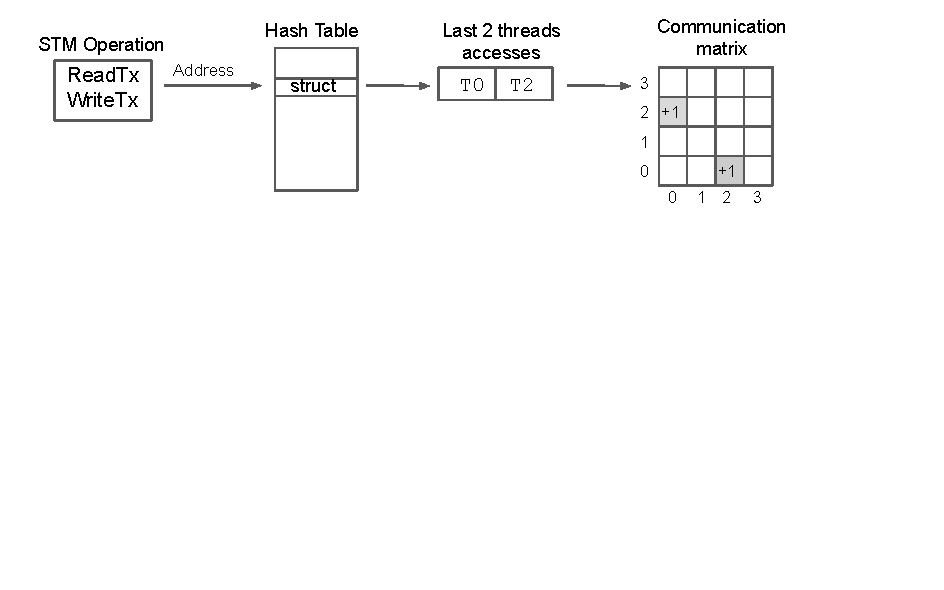
\includegraphics[width=\fullImageWidth\textwidth,trim=10 170 60 0,clip]{figures/mechanism/mechanism.pdf}
	}
	\caption{Mechanism for detecting communication patterns. Data structures are shown for an application consisting of 4 threads (0-3.)}
	\label{fig:mechanism}
\end{figure}


\begin{figure}[!ht]
	%https://docs.google.com/presentation/d/1PTBP2GqremN_1nalfXQhCORR1nwgsHspnoNh1o6fKCI/edit#slide=id.g961e369ddb_3_0
	\centering
	\fbox{
		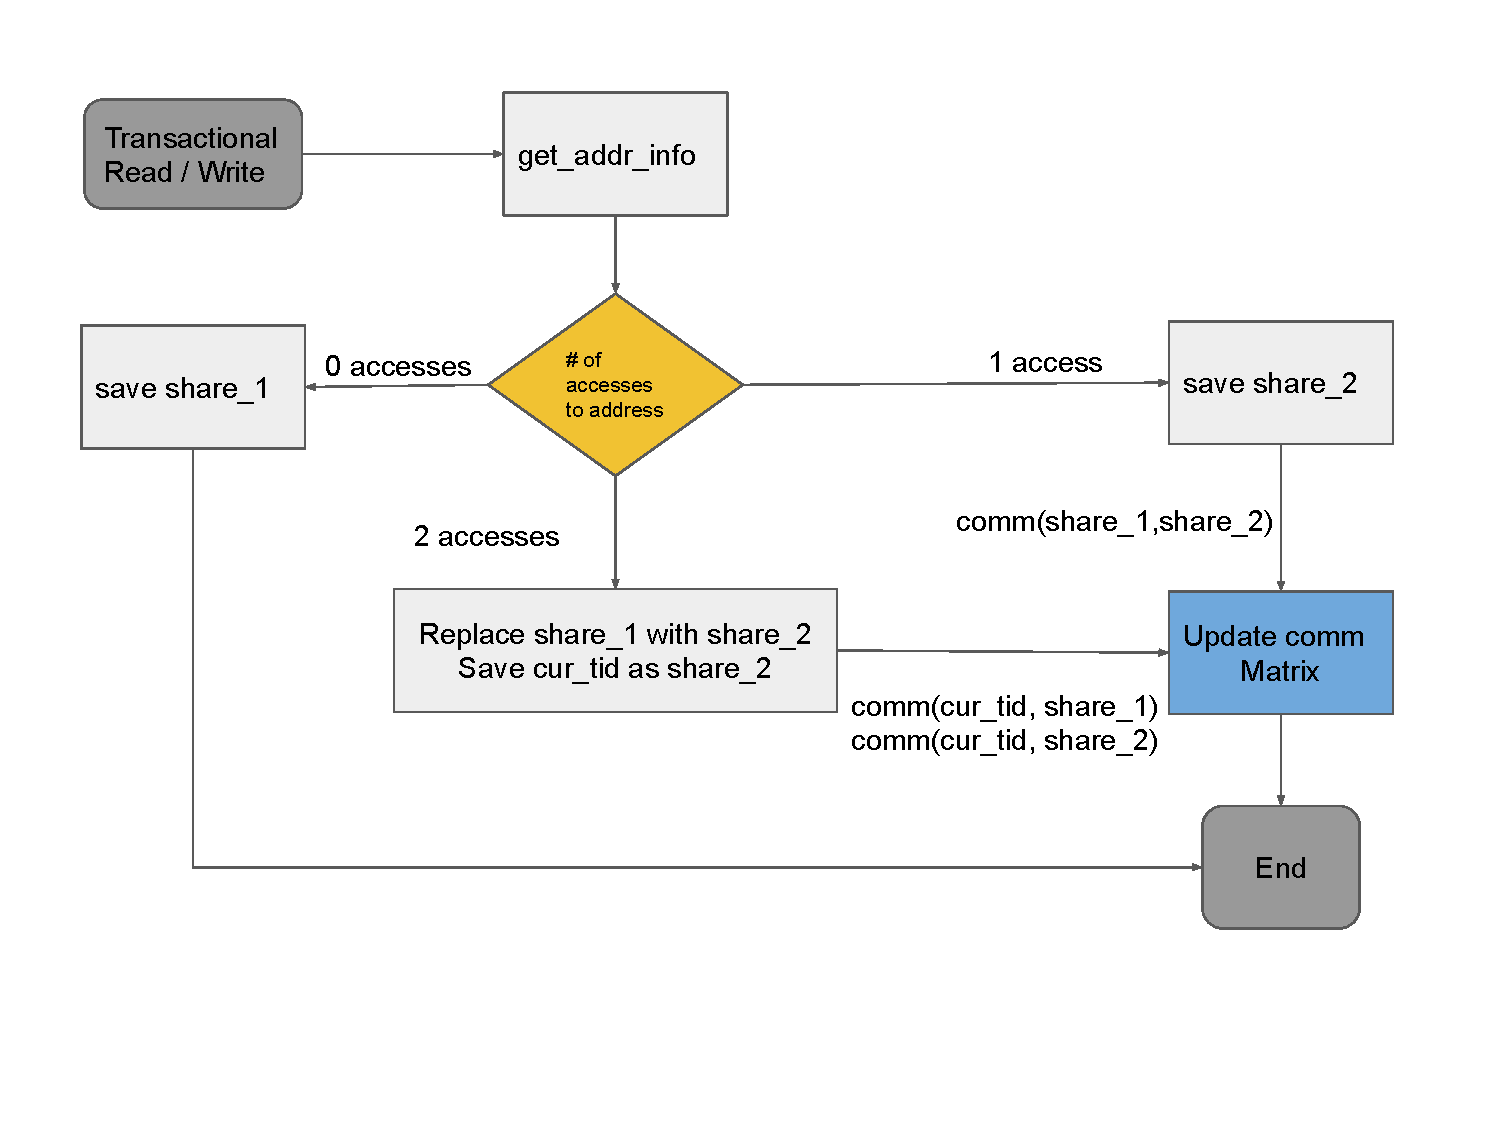
\includegraphics[width=\fullImageWidth\textwidth,trim=20 80 30 30,clip]{figures/mechanism/mechanism-fluxogram.pdf}
		%		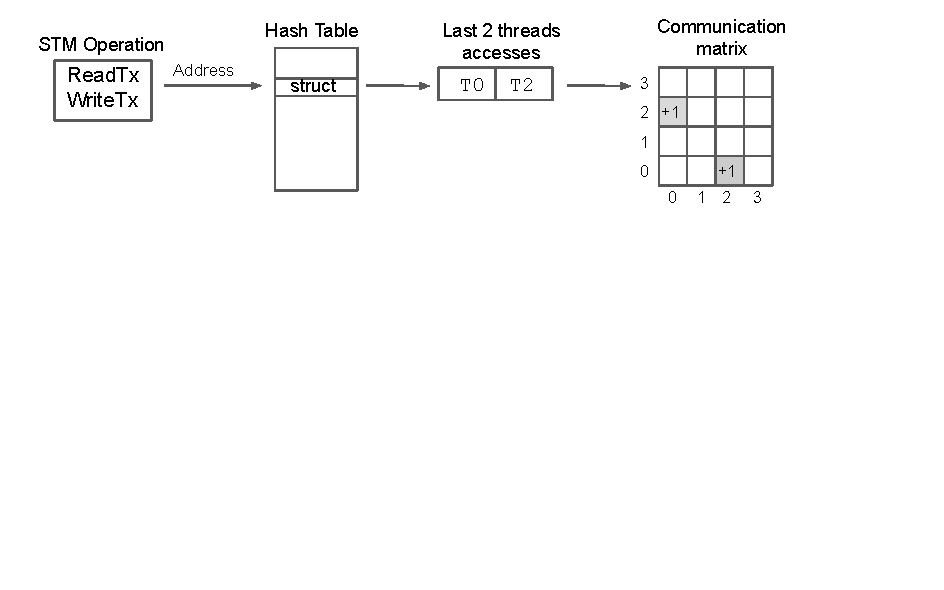
\includegraphics[width=\fullImageWidth\textwidth]{figures/mechanism/mechanism.png}
	}
	\caption{Flowchart of the proposed mechanism.}
	\label{fig:mechanism-fluxogram}
\end{figure}

\begin{algorithm}[!ht]
	\caption{Detecting communication patterns.}\label{alg:detectcomm}
%	\small
	\begin{algorithmic}[1]
		\Require
		\Statex \textbf{addr}: memory address being accessed
		\Statex \textbf{tid}: thread ID of the thread that is accessing the address
		\Statex
		\LineComment{\texttt{elem} is a struct that stores the memory address and the last 2 threads that have accessed it}
		\State $elem \gets \text{getAddressInfo}(addr)$ \label{alg1:elem}
		\State $accesses \gets \text{getAccesses}(elem)$ \label{alg1:count}
		\If {$(accesses = 0)$} \Comment{First access to the address} \label{alg1:0acc}
		\State $elem.t1 \gets tid$ \label{alg1:0accStore}
		% \EndIf
		\ElsIf {($accesses = 1$)}  \Comment{One previous access} \label{alg1:1acces}
		\If {($elem.t1 \neq tid$)} \label{alg1:1accesDiff}
		\State $\text{update\_comm\_matrix}(tid, \ elem.t1)$ \label{alg1:1accesComm}
		\State $elem.t2 \gets elem.t1$ \label{alg1:1accest2}
		\State $elem.t1 \gets tId$ \label{alg1:1accest1}
		% \EndIf
		\EndIf
		\ElsIf {($accesses = 2$)} \Comment{Two previous accesses} \label{alg1:2acces}
		\If {($elem.t1 \neq tid$)  \textbf{and} ($elem.t2 \neq tid$)} \label{alg1:2acces2diff}
		\State $\text{update\_comm\_matrix}(tid, \ elem.t1)$ \label{alg1:2acces2diffupt1}
		\State $\text{update\_comm\_matrix}(tid, \ elem.t2)$ \label{alg1:2acces2diffupt2}
		\State $elem.t2 \gets elem.t1$ \label{alg1:2acces2diffdel}
		\State $elem.t1 \gets tid$
		\ElsIf {($elem.t1 = tid$)} \label{alg1:2acces1difft2}
		\State $\text{update\_comm\_matrix}(tid, \ elem.t2)$
		\ElsIf {($elem.t2 = tid$)} \label{alg1:2acces1difft1}
		\State $\text{update\_comm\_matrix}(tid, \ elem.t1)$
		\State $elem.t2 \gets elem.t1$ \label{alg1:2acces1difft1del}
		\State $elem.t1 \gets tid$
		% \EndIf
		\EndIf
		\EndIf
	\end{algorithmic}
\end{algorithm}

Our mechanism to detect the communication pattern of an application is shown in Figures~\ref{fig:mechanism}--\ref{fig:mechanism-fluxogram} and detailed in Algorithm~\ref{alg:detectcomm}. This mechanism is executed before each transactional read or write operation. To keep track of accessed addresses, a hash table is used, in which keys are memory addresses. Each position of the hash table contains a structure with the memory address and the last 2 threads that have accessed it. Following the intuition of previous work, we store only the last 2 thread access, to avoid false temporal communication~\cite{Diener:2016:2}. In case of hash conflicts, a linked list with all memory addresses with the same hash is kept. In line~\ref{alg1:elem}, the function \texttt{getAddressInfo} gets from the hash table the structure containing information about the address being accessed. The next step is to get how many accesses this address had before the current one (line \ref{alg1:count}). If it is the first access (line \ref{alg1:0acc}), we only store the thread that is accessing it (line \ref{alg1:0accStore}), i.e., no communication events have happened yet. The next case is if the address had one access before the current (line \ref{alg1:1acces}) and it was made by a different thread (line \ref{alg1:1accesDiff}). If true, we have a communication event. In that case, we call the function \texttt{update\_comm\_matrix} (line \ref{alg1:1accesComm}) to update the communication matrix, increasing the amount of communication between the two threads. The matrix is square and symmetric because the amount of communication, for instance, between threads 0 and 2 is the same from 2 and 0 (\figurename~\ref{fig:mechanism}). Also, the matrix has an order equal to the maximum number of threads. Using the matrix, we update the threads that accessed the address (lines \ref{alg1:1accest2} and \ref{alg1:1accest1}). It is worth noting that write accesses to the communication matrix are not synchronized. This decision was made because the high overhead involved to synchronize the access. Besides, the collateral effects expected due to the parallel updates on the matrix, for instance, incorrect pairs of thread being incorrectly updated in the matrix, are considered eventual and not harmful to the mechanism.

The final case is if the address had 2 previous accesses (line \ref{alg1:2acces}), then there are 3 sub-cases. The first one is if the current thread accessing the address is different from the 2 previous (line \ref{alg1:2acces2diff}). In that case, we have a third distinct thread accessing the address, and we update the communication matrix between the 3 (lines \ref{alg1:2acces2diffupt1} and \ref{alg1:2acces2diffupt2}). After that, the oldest access is removed (line \ref{alg1:2acces2diffdel}). However, if the test of the line \ref{alg1:2acces2diff} was false, it means that the current thread accessing the address is the same from a previous one. In that case, we need to check which thread is accessing again (lines \ref{alg1:2acces1difft2} and \ref{alg1:2acces1difft1}), and update the communication matrix correctly. Also, since we keep only the last 2 accesses to the memory address, when a third thread access the address, it is necessary to replace the oldest one (line \ref{alg1:2acces1difft1del}).

\section{Implementation}\label{sec:implement}

We implemented our proposed mechanism inside the state-of-art STM library \texttt{TinySTM}~\cite{TinySTM2}, version 1.0.5. The majority of the modifications were made in the file \texttt{stm\_internal.h}. The Algorithm~\ref{alg:detectcomm} is called inside the functions \texttt{stm\_write} and \texttt{stm\_load} from \texttt{TinySTM}. 

\section{Evaluation}

This section describes experiments made in order to evaluate the proposed mechanism to detect the sharing behavior of STM applications.

\subsection{Methodology}\label{sec:mechMethodology}

We used the proposed mechanism to collect the communication matrices of STM applications by using the modified version of the \texttt{TinySTM} library (Section~\ref{sec:implement}), with the default options: \emph{lazy} version management, \emph{eager} conflict detection and contention manager \emph{suicide}.

\begin{table}[!tb]
	\small
	\centering
	\caption{Default arguments for the programs used in the experiments.}
	\label{tab:defaultParams}
	\begin{tabularx}{\textwidth}{@{}lXl@{}}
		\toprule
		Application & Arguments                                          \\ \midrule
		bayes                & \texttt{-v32 -r8192 -n10 -p40 -i2 -e8 -s1 -t \thNumber}                \\
		genome               & \texttt{-g49152 -s256 -n33554432 -t \thNumber}                         \\
		intruder             & \texttt{-a10 -l128 -n262144 -s1 -t \thNumber}                          \\
		kmeans               & \texttt{-m40 -n40 -t0.00001 -i random-n65536-d32-c16.txt -p \thNumber}\\
		labyrinth            & \texttt{-i random-x1024-y1024-z9-n1024.txt -t \thNumber}               \\
		ssca2                & \texttt{-s21 -i1.0 -u1.0 -l3 -p3 -t \thNumber}                         \\
		vacation             & \texttt{-n4 -q90 -u100 -r1310720 -t16777216 -c \thNumber}              \\
		yada                 & \texttt{-a15 -i ttimeu1000000.2 -t \thNumber}                          \\
		redblacktree			& \texttt{-u 20 -i 1000000 -d 500000000 -n \thNumber}                          \\
		hashmap			& \texttt{-u 20 -i 1000000 -d 500000000 -n \thNumber}                          \\
		\bottomrule
	\end{tabularx}
\end{table}

The applications used in the experiments were all eight benchmarks from the Stanford Transactional Applications for Multi-Processing (\texttt{STAMP})~\cite{STAMP} version 0.9.10, and two micro-benchmarks (HashMap and Redblacktree) from \citeNamesYearPar{Diegues:2014:2}. The input arguments used to run each application are shown in \tablename~\ref{tab:defaultParams}. Most parameters are larger than the largest ones suggested in the original paper~\cite{STAMP} to achieve more substantial execution times on modern machines. To run the experiments, we used the the following NUMA machine (node distances were gathered with \texttt{numactl}~\cite{libnuma}):

\begin{itemize}
	\item \textbf{Xeon}: 8 Intel Xeon E5-4650 processors and 488 GiB of RAM running Linux kernel 4.19.0-9. Each CPU has 12 2-HT cores, totaling 96 cores. Each CPU corresponds to a NUMA node (for a total of 8 NUMA nodes), and 12$\times$ 32 KB L1d, 12$\times$ 32 KB L1i, 12$\times$ 256 KB L2 and 30 MB L3 cache. Node distances: 50 -- 65. Applications were compiled using gcc 8.3.0.
\end{itemize}

\subsection{Communication matrices}\label{sect:StampMatrices}
Figures~\ref{fig:commMatrOpt16}--\ref{fig:commMatrXeon96} shown the collected communication matrices using the proposed mechanism for 16, 32, 64 and 96 threads. In the figures, axes show threads IDs and darker cells indicate more communication between pairs of threads.
\begin{figure}[ht]
	\centering
	\subfigure[bayes]{
		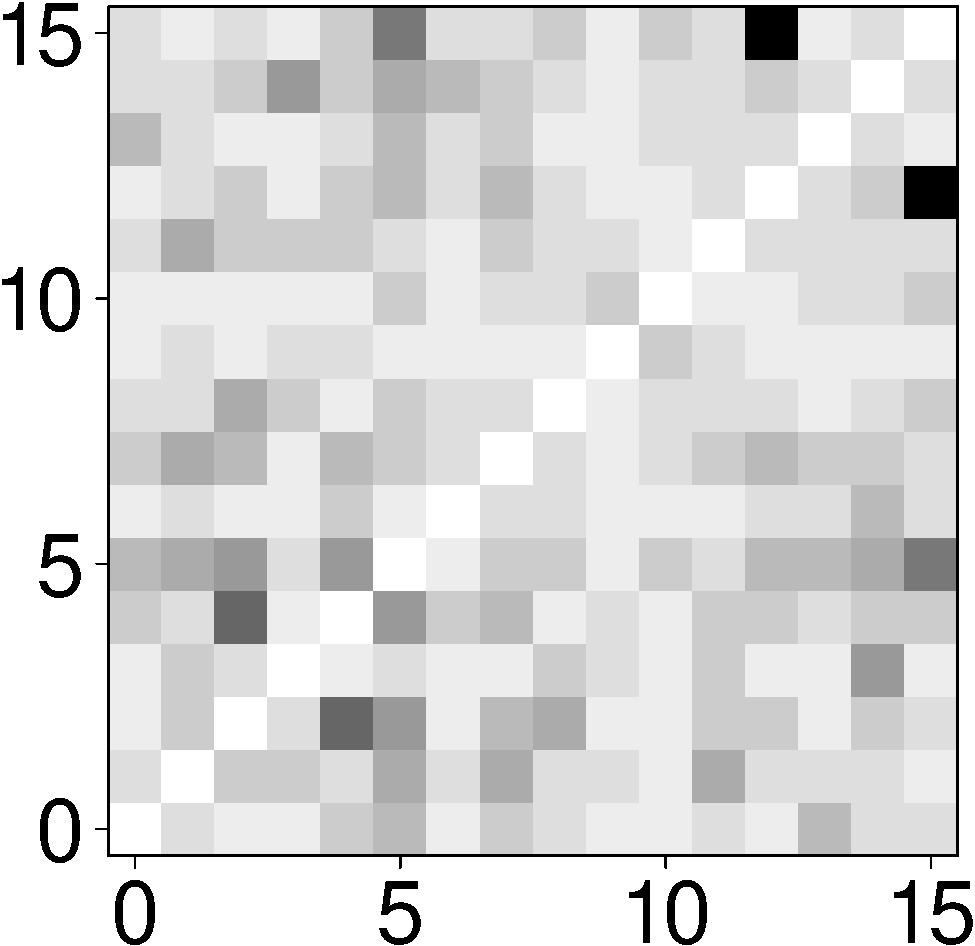
\includegraphics[width=\oneFPage\textwidth]{figures/mechanism/matrices/opteron/bayes_16.pdf}
	}
	\subfigure[genome]{
		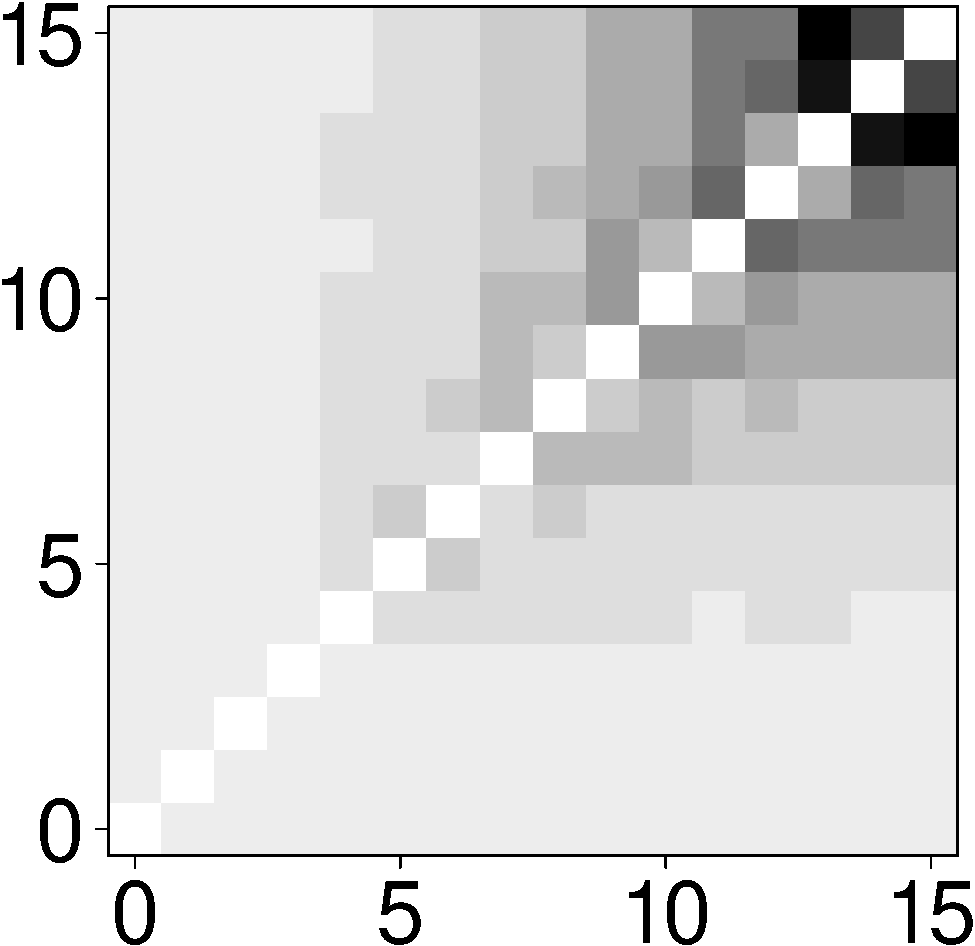
\includegraphics[width=\oneFPage\textwidth]{figures/mechanism/matrices/opteron/genome_16.pdf}
	}
	\subfigure[intruder]{
		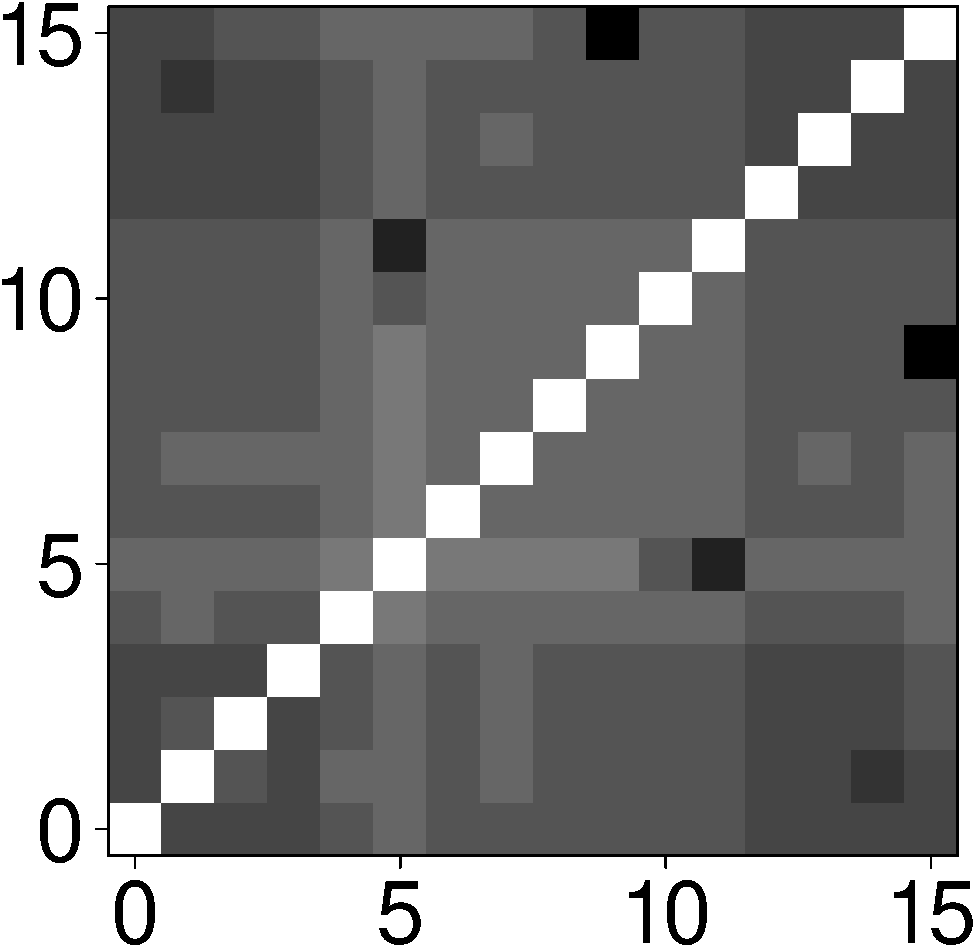
\includegraphics[width=\oneFPage\textwidth]{figures/mechanism/matrices/opteron/intruder_16.pdf}
	}
	\subfigure[kmeans]{
		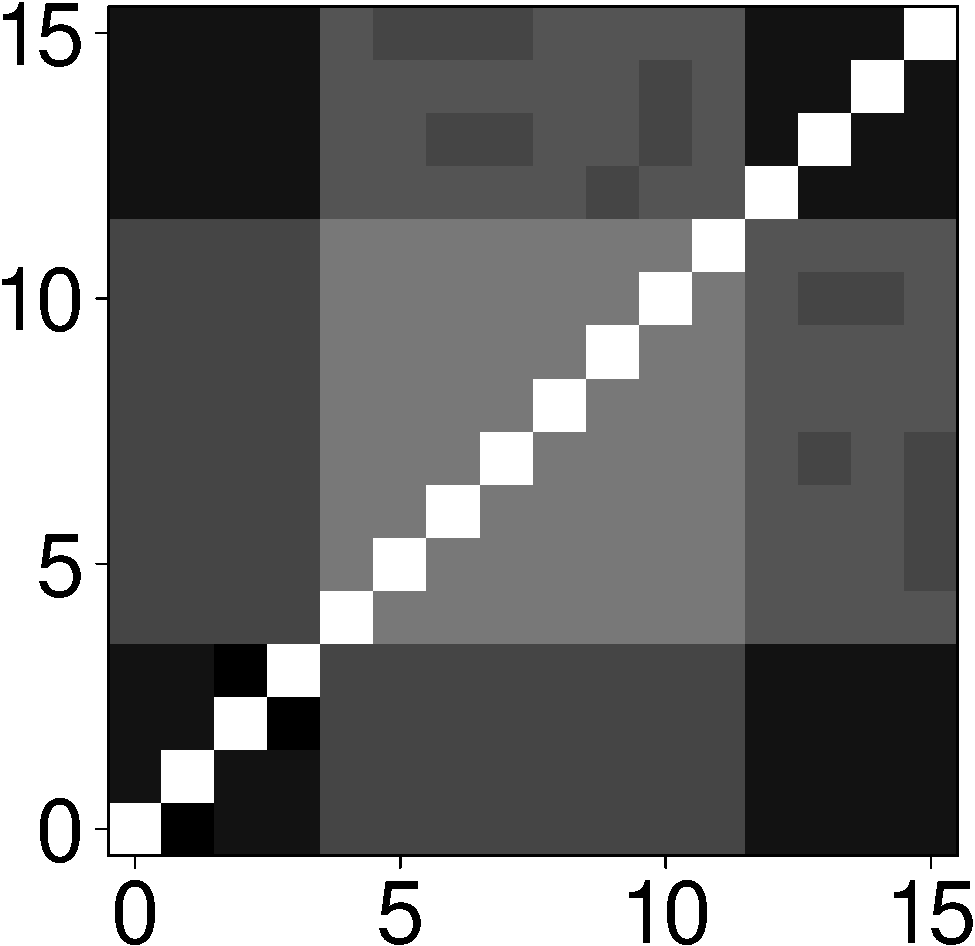
\includegraphics[width=\oneFPage\textwidth]{figures/mechanism/matrices/opteron/kmeans_16.pdf}
	}
	\subfigure[labyrinth]{
		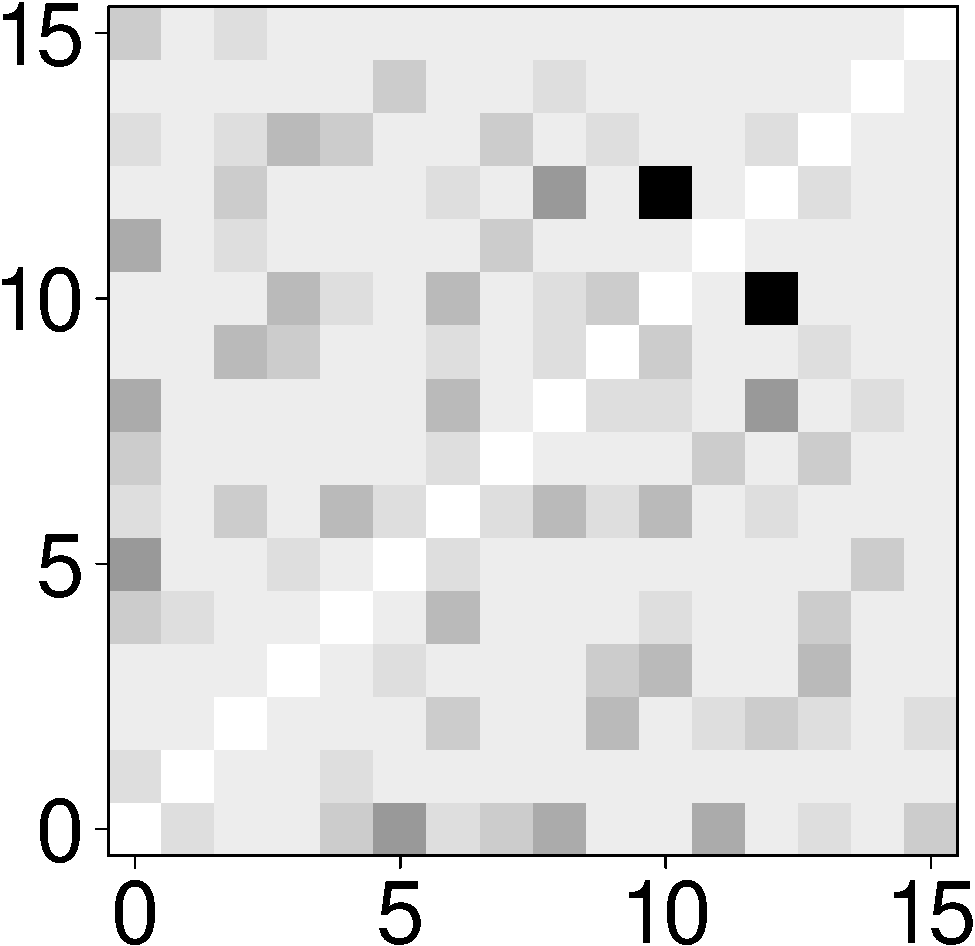
\includegraphics[width=\oneFPage\textwidth]{figures/mechanism/matrices/opteron/labyrinth_16.pdf}
	}
	\\
	\subfigure[ssca2]{
		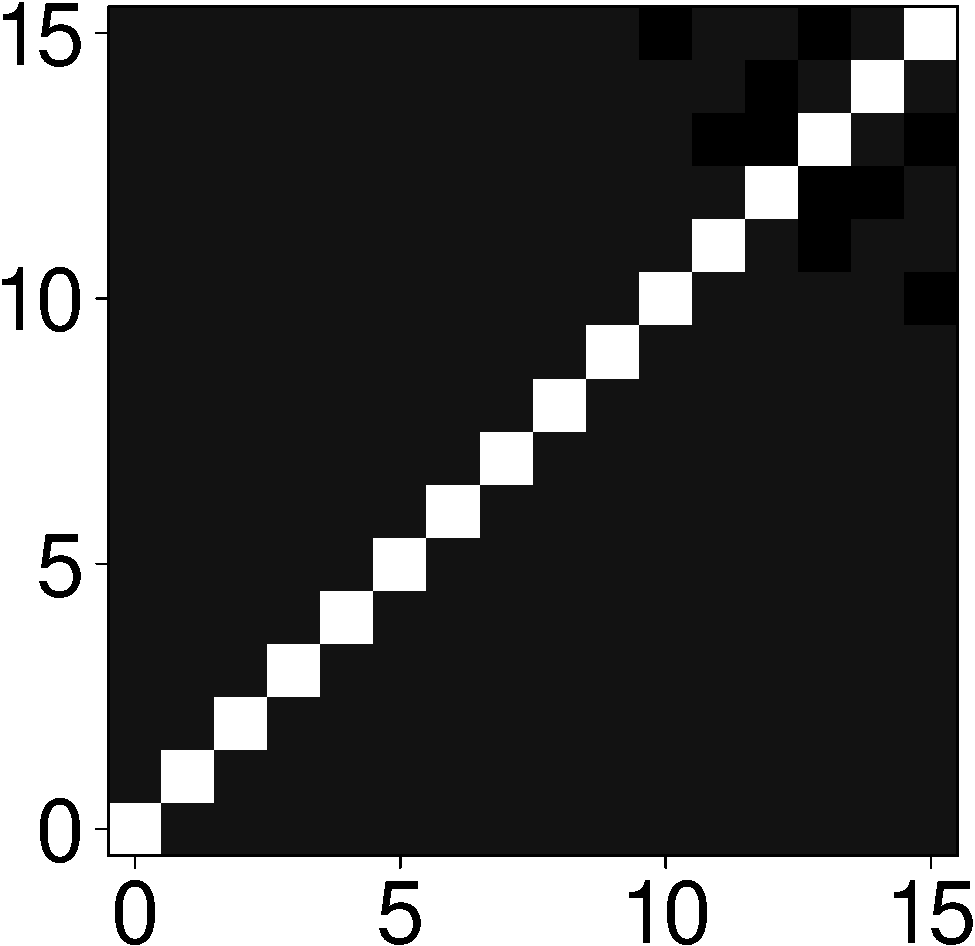
\includegraphics[width=\oneFPage\textwidth]{figures/mechanism/matrices/opteron/ssca2_16.pdf}
	}
	\subfigure[vacation]{
		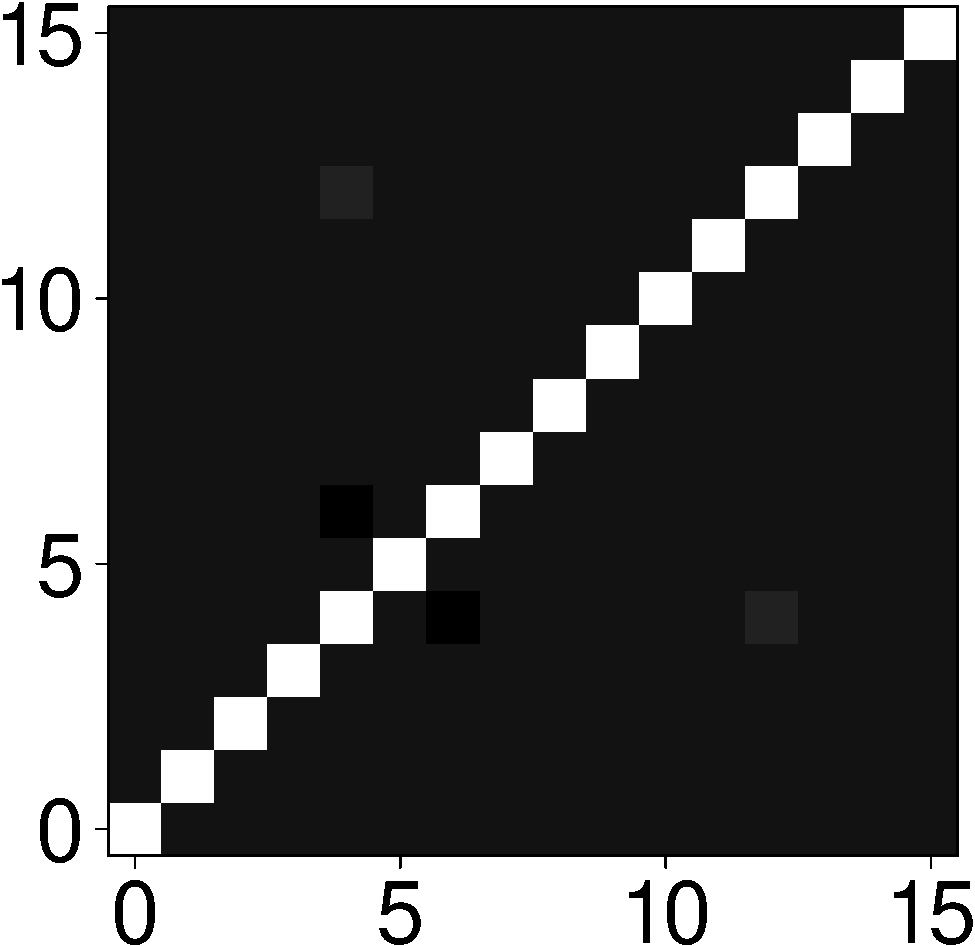
\includegraphics[width=\oneFPage\textwidth]{figures/mechanism/matrices/opteron/vacation_16.pdf}
	}
	\subfigure[yada]{
		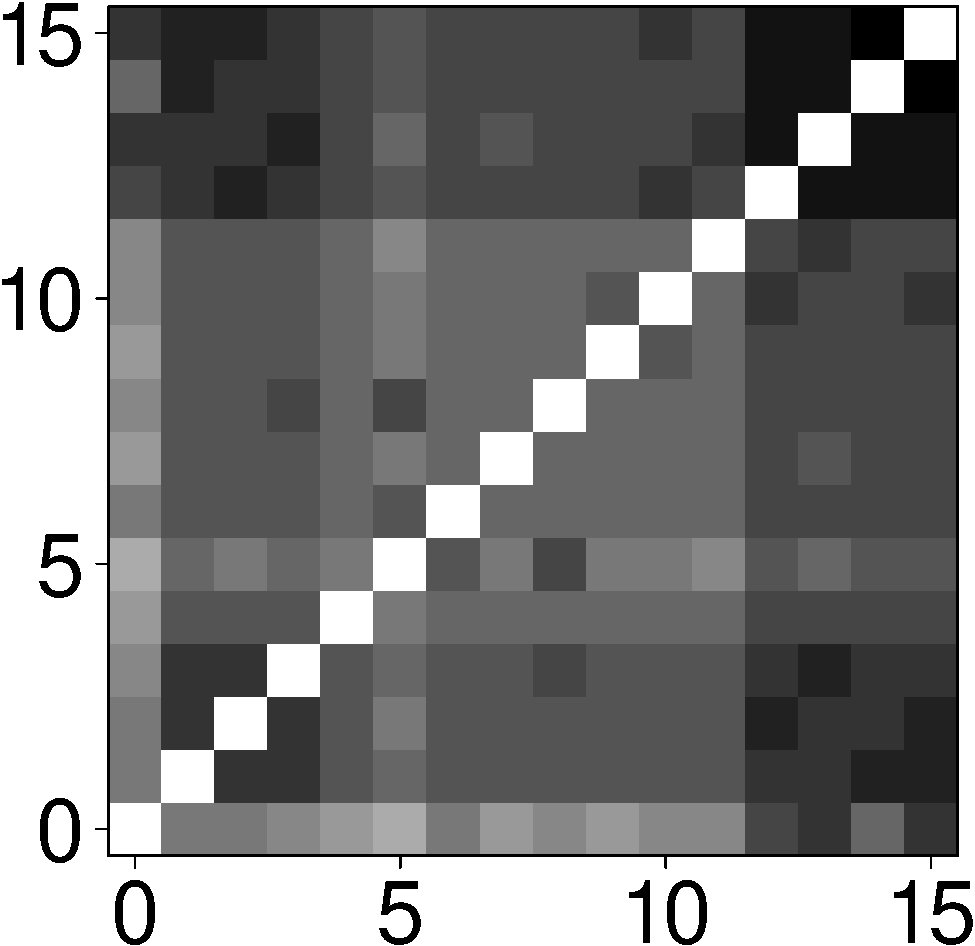
\includegraphics[width=\oneFPage\textwidth]{figures/mechanism/matrices/opteron/yada_16.pdf}
	}
	\subfigure[redblacktree]{
		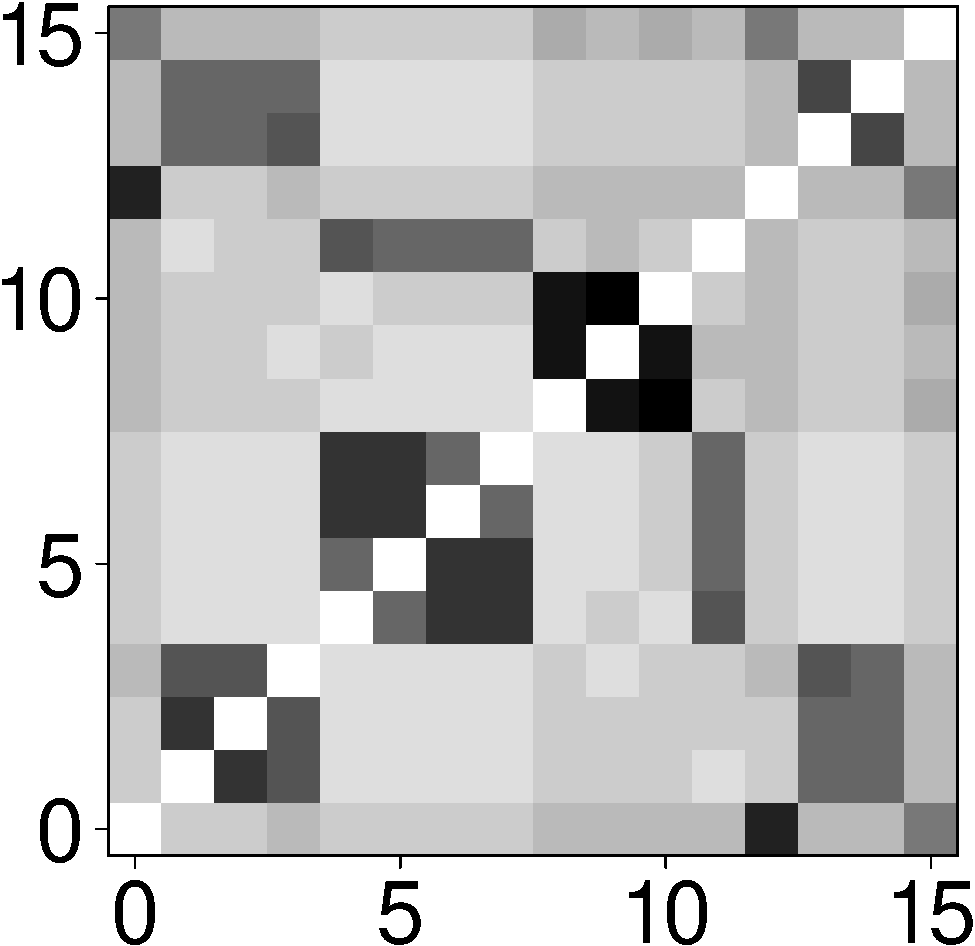
\includegraphics[width=\oneFPage\textwidth]{figures/mechanism/matrices/opteron/redblacktree_16.pdf}
	}
	\subfigure[hashmap]{
		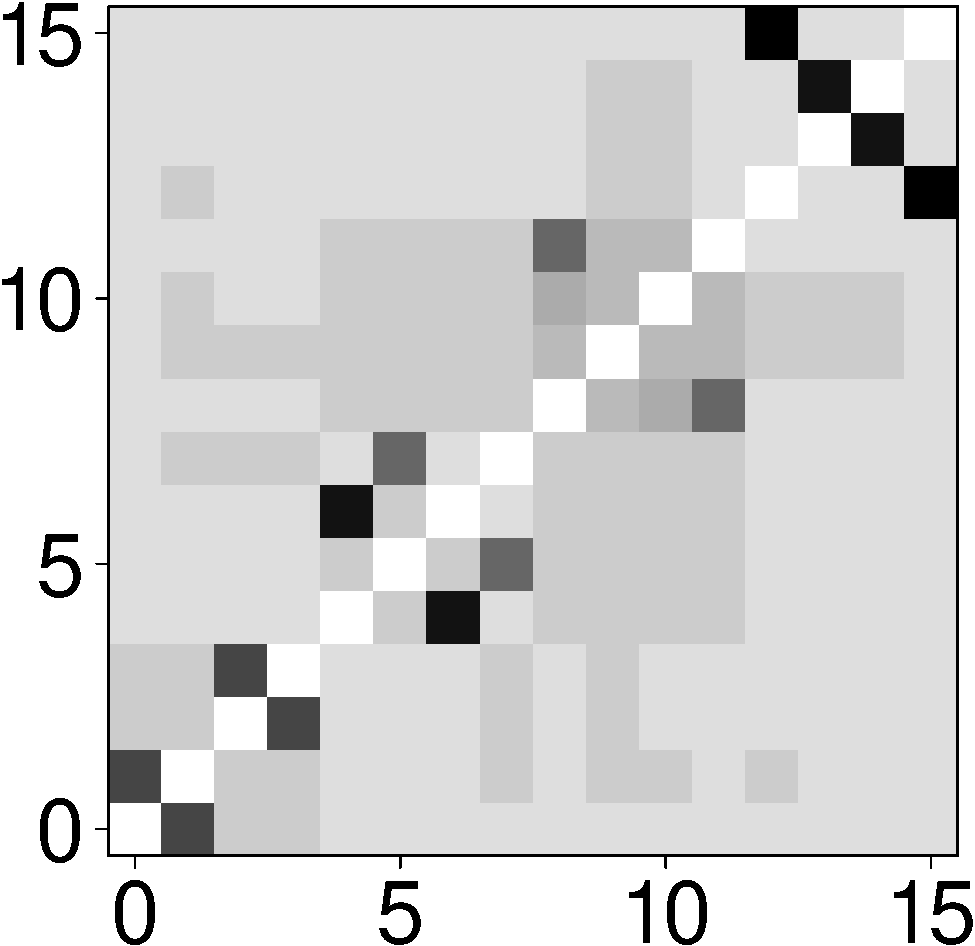
\includegraphics[width=\oneFPage\textwidth]{figures/mechanism/matrices/opteron/hashmap_16.pdf}
	}
	\caption{Communication matrices - 16 threads.}
	\label{fig:commMatrOpt16}
\end{figure}

\begin{figure}[!bt]
	\centering
	\subfigure[bayes]{
		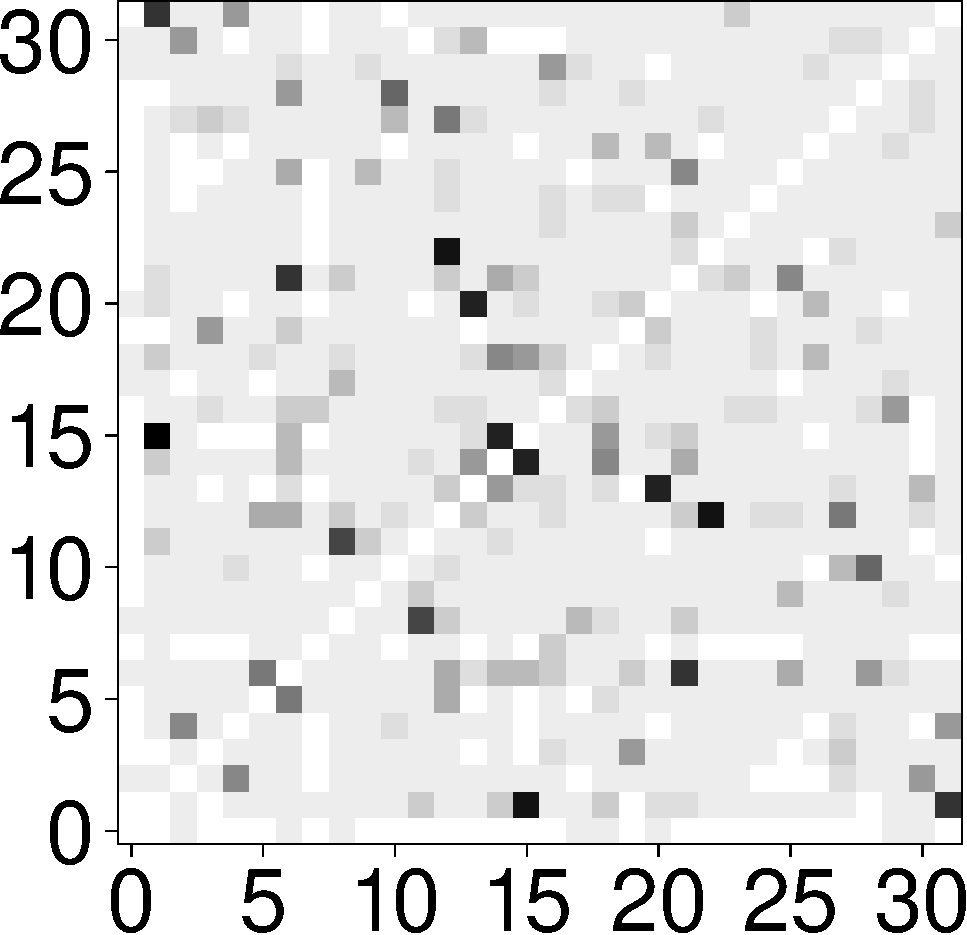
\includegraphics[width=\oneFPage\textwidth]{figures/mechanism/matrices/xeon/bayes_32.pdf}
	}
	\subfigure[genome]{
		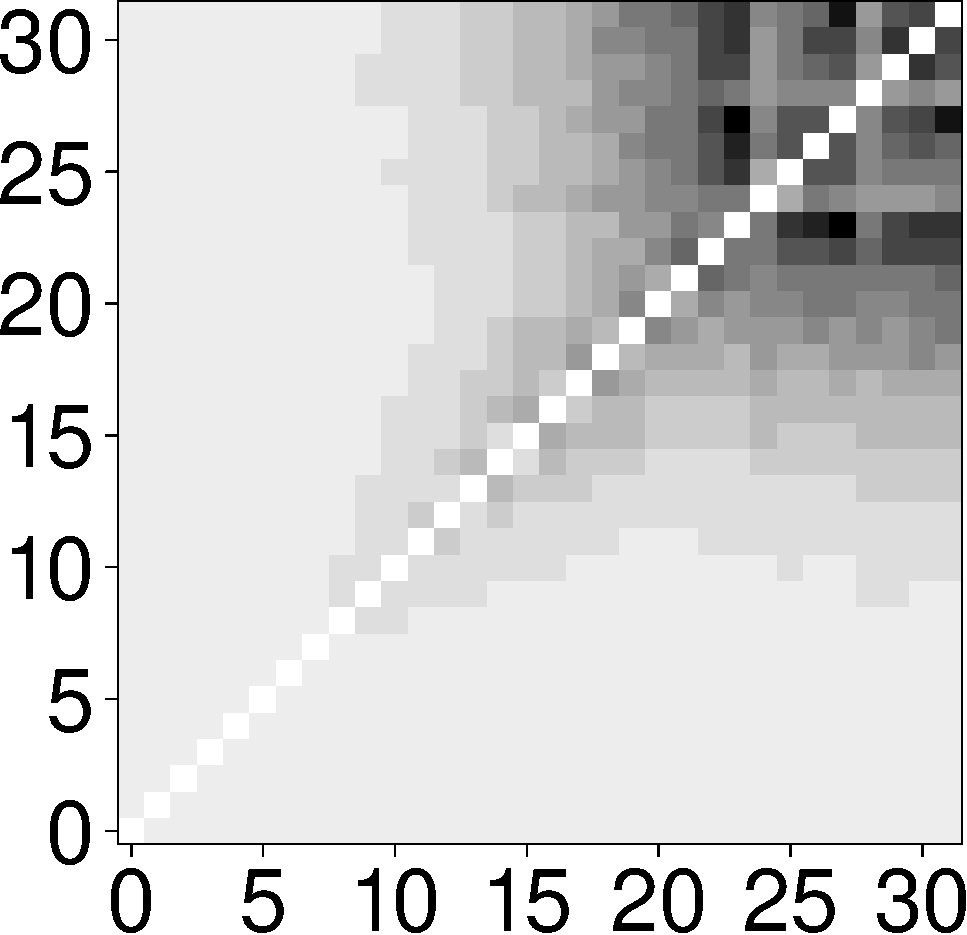
\includegraphics[width=\oneFPage\textwidth]{figures/mechanism/matrices/xeon/genome_32.pdf}
	}
	\subfigure[intruder]{
		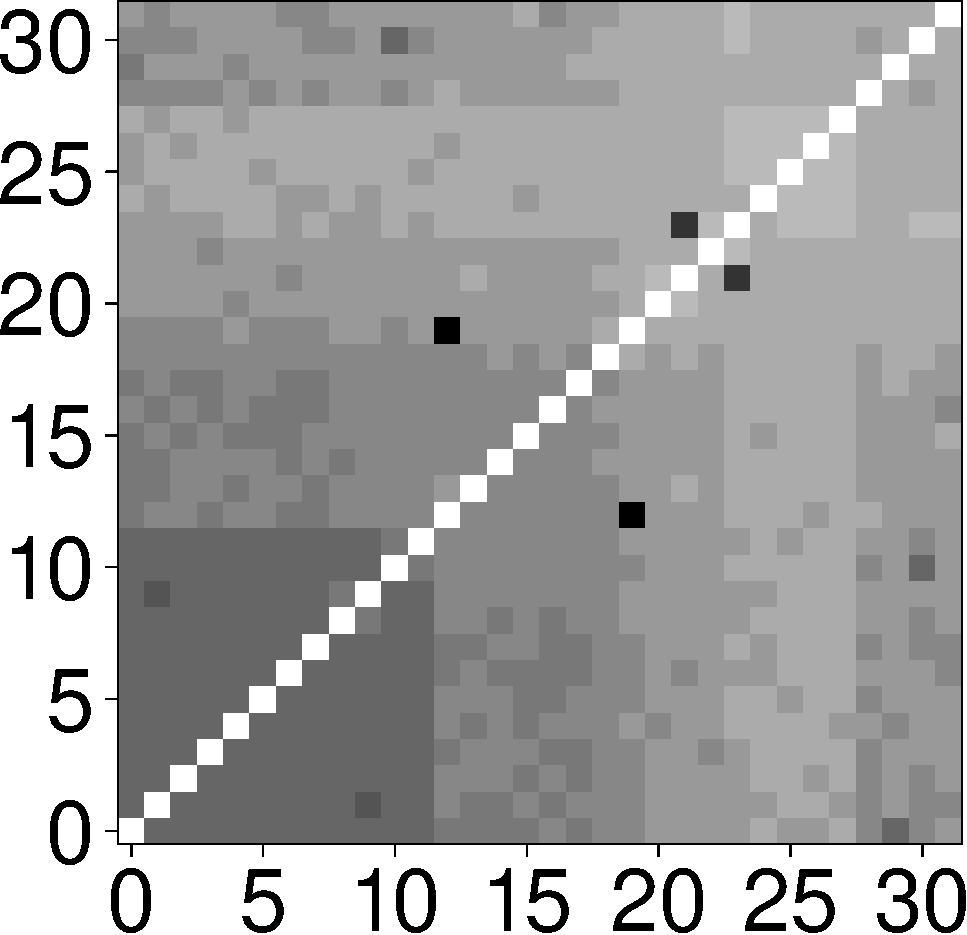
\includegraphics[width=\oneFPage\textwidth]{figures/mechanism/matrices/xeon/intruder_32.pdf}
	}
	\subfigure[kmeans]{
		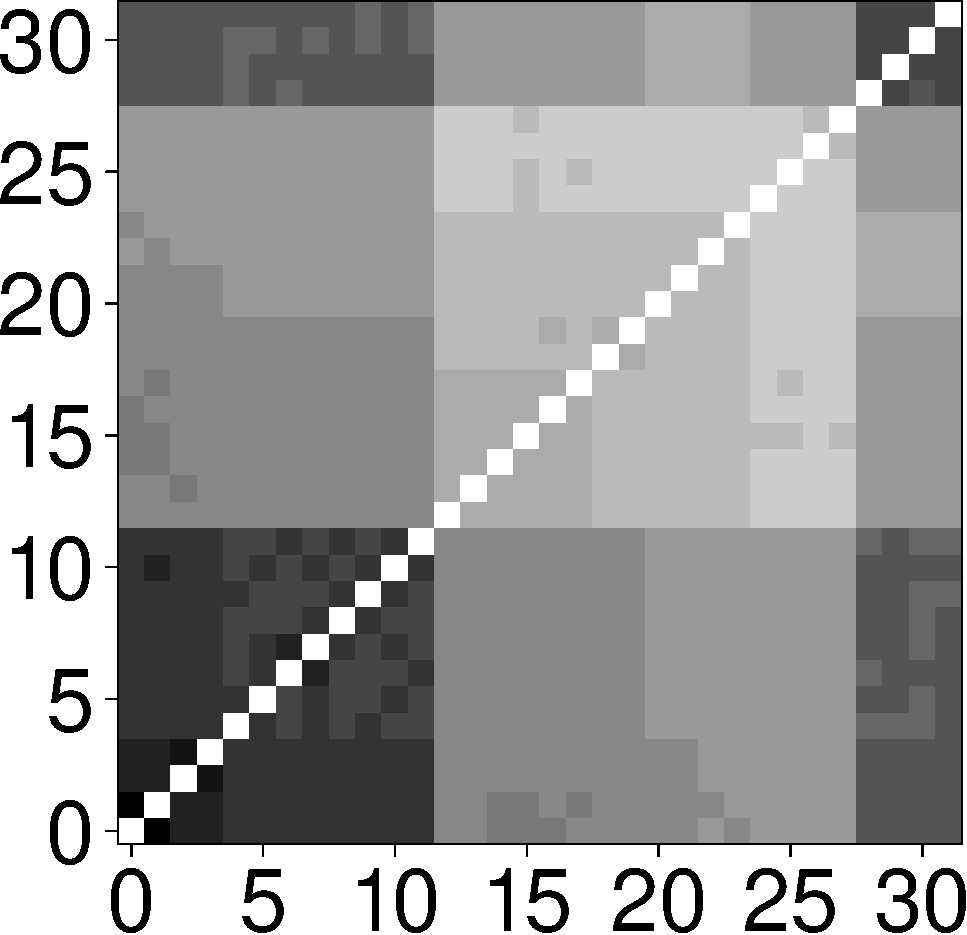
\includegraphics[width=\oneFPage\textwidth]{figures/mechanism/matrices/xeon/kmeans_32.pdf}
	}
	\subfigure[labyrinth]{
		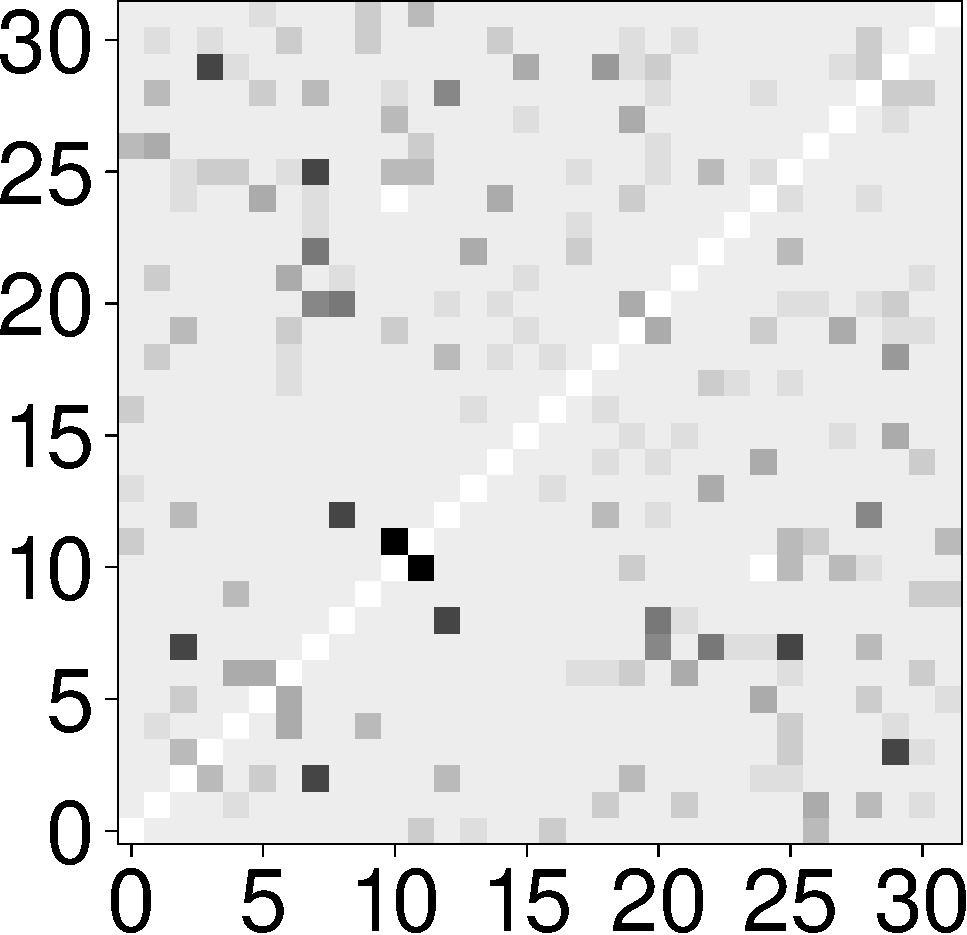
\includegraphics[width=\oneFPage\textwidth]{figures/mechanism/matrices/xeon/labyrinth_32.pdf}
	}
\\
	\subfigure[ssca2]{
		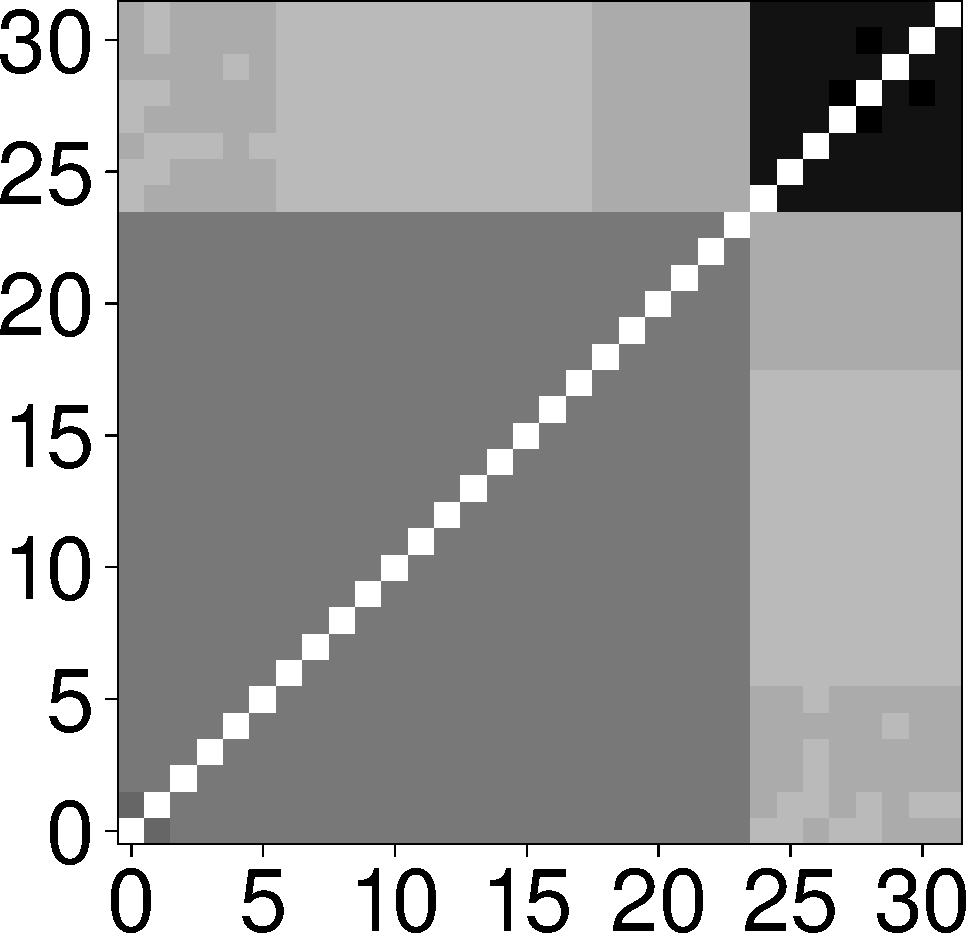
\includegraphics[width=\oneFPage\textwidth]{figures/mechanism/matrices/xeon/ssca2_32.pdf}
	}
	\subfigure[vacation]{
		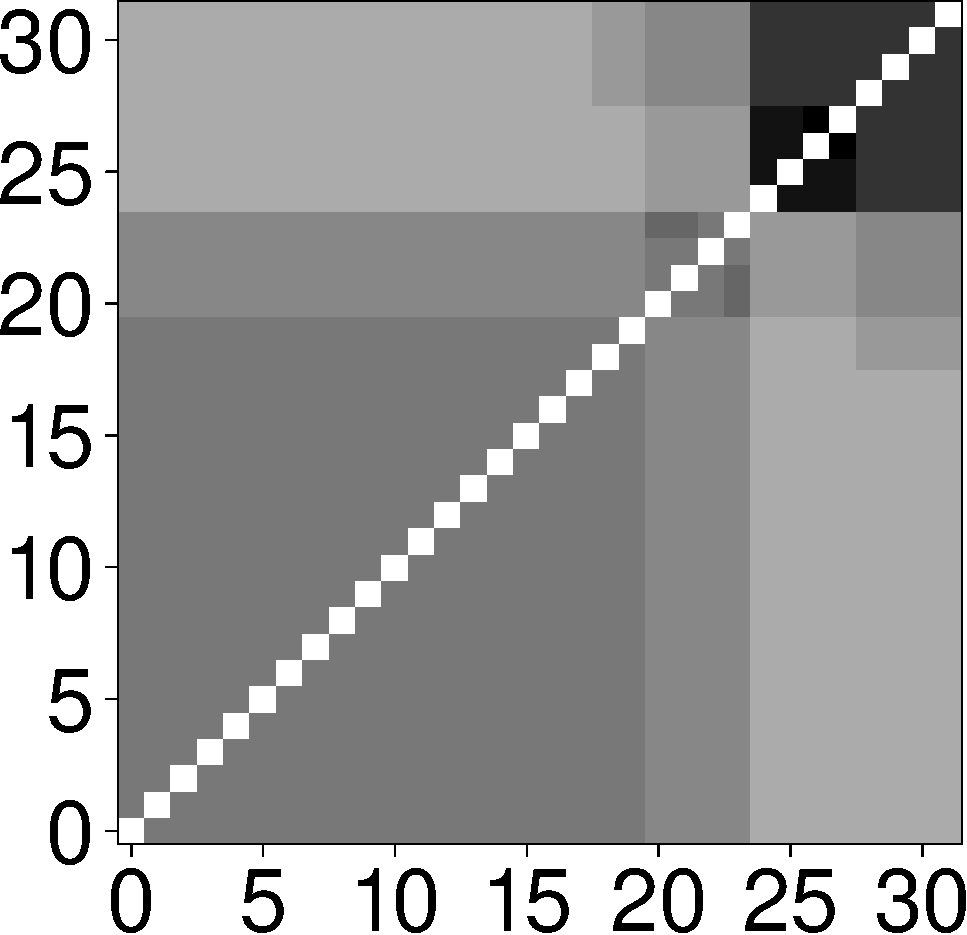
\includegraphics[width=\oneFPage\textwidth]{figures/mechanism/matrices/xeon/vacation_32.pdf}
	}
	\subfigure[yada]{
		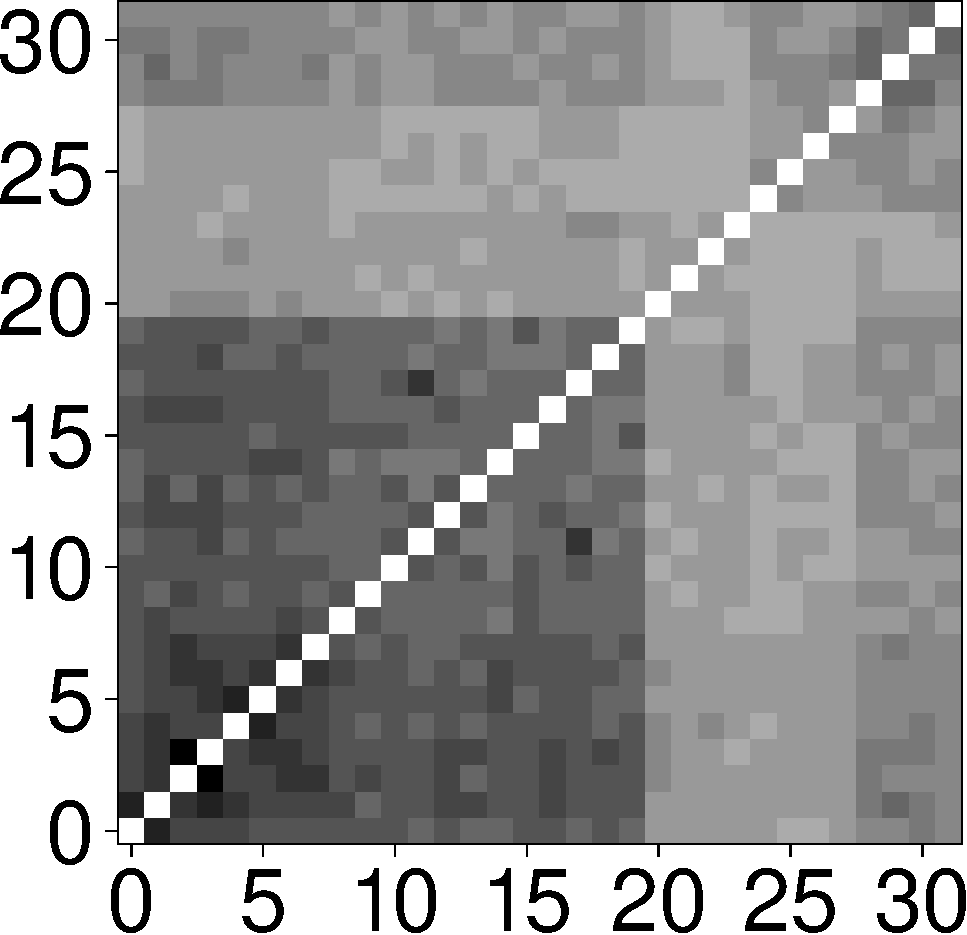
\includegraphics[width=\oneFPage\textwidth]{figures/mechanism/matrices/xeon/yada_32.pdf}
	}
	\subfigure[redblacktree]{
		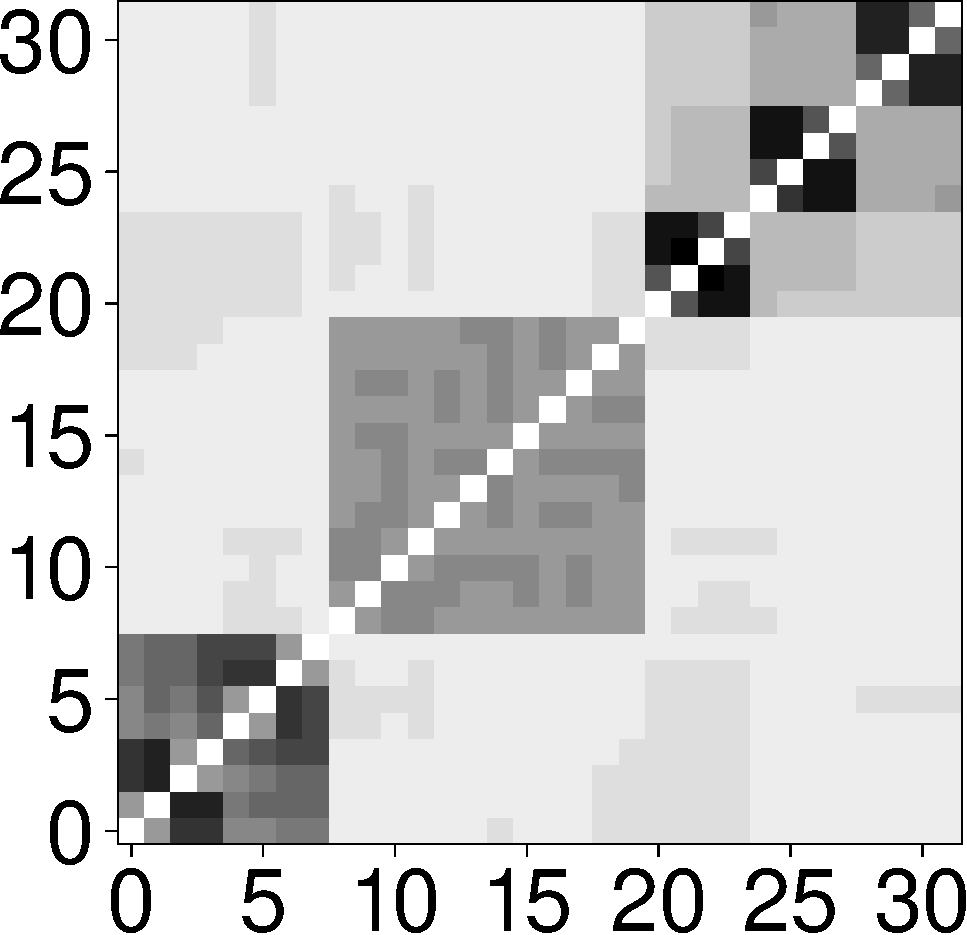
\includegraphics[width=\oneFPage\textwidth]{figures/mechanism/matrices/xeon/redblacktree_32.pdf}
	}
	\subfigure[hashmap]{
		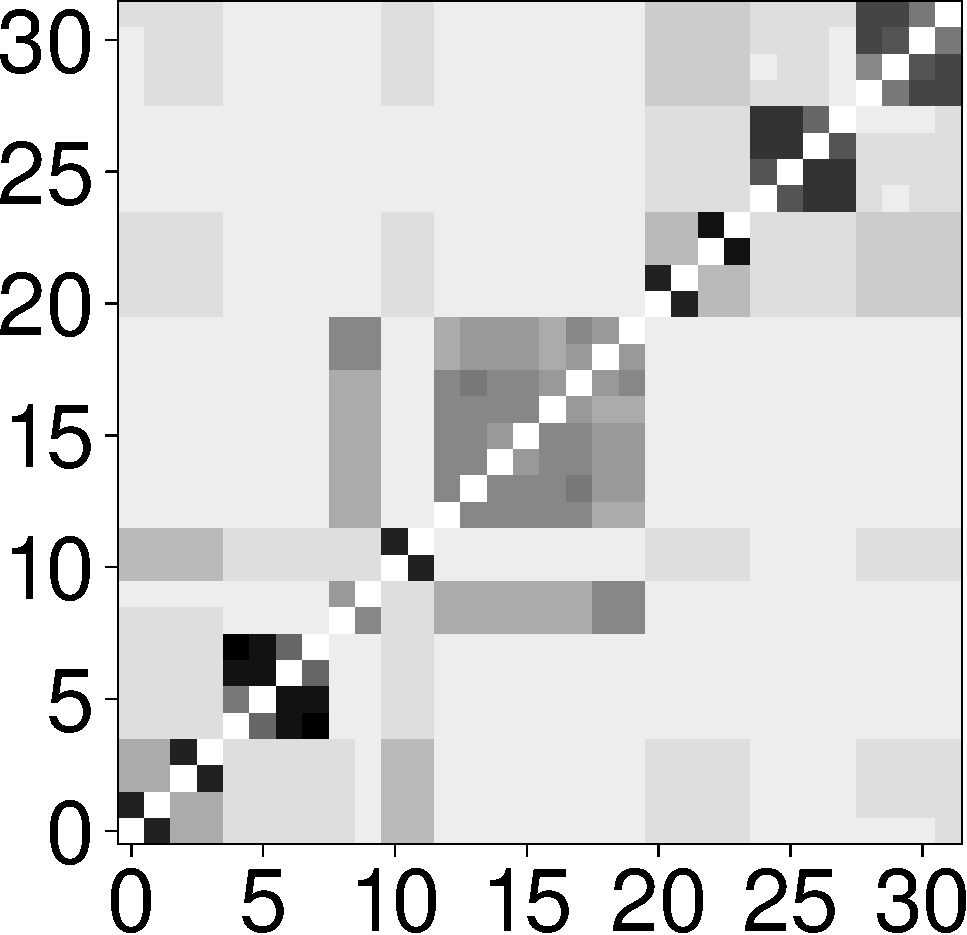
\includegraphics[width=\oneFPage\textwidth]{figures/mechanism/matrices/xeon/hashmap_32.pdf}
	}
	\caption{Communication matrices - 32 threads.}
\end{figure}

%%%%%%%%%%%%%%%%%%%

\begin{figure}[!bt]
	\centering
	\subfigure[bayes]{
		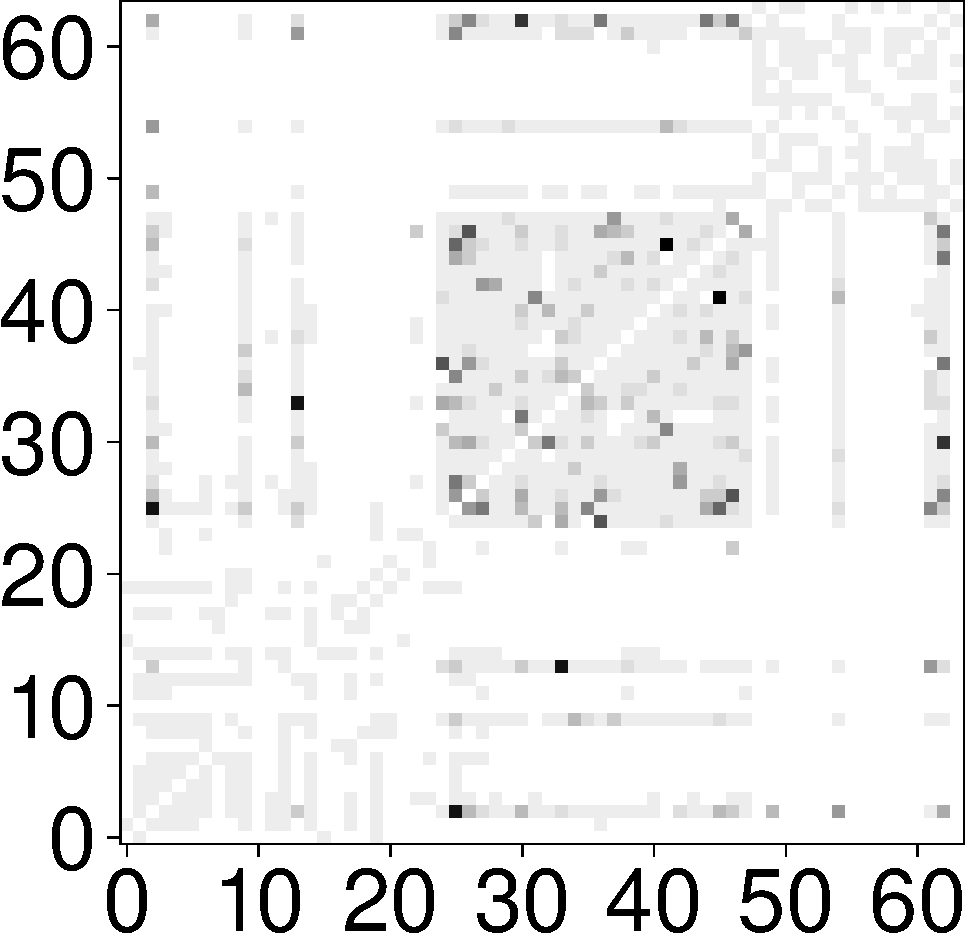
\includegraphics[width=\oneFPage\textwidth]{figures/mechanism/matrices/xeon/bayes_64.pdf}
	}
	\subfigure[genome]{
		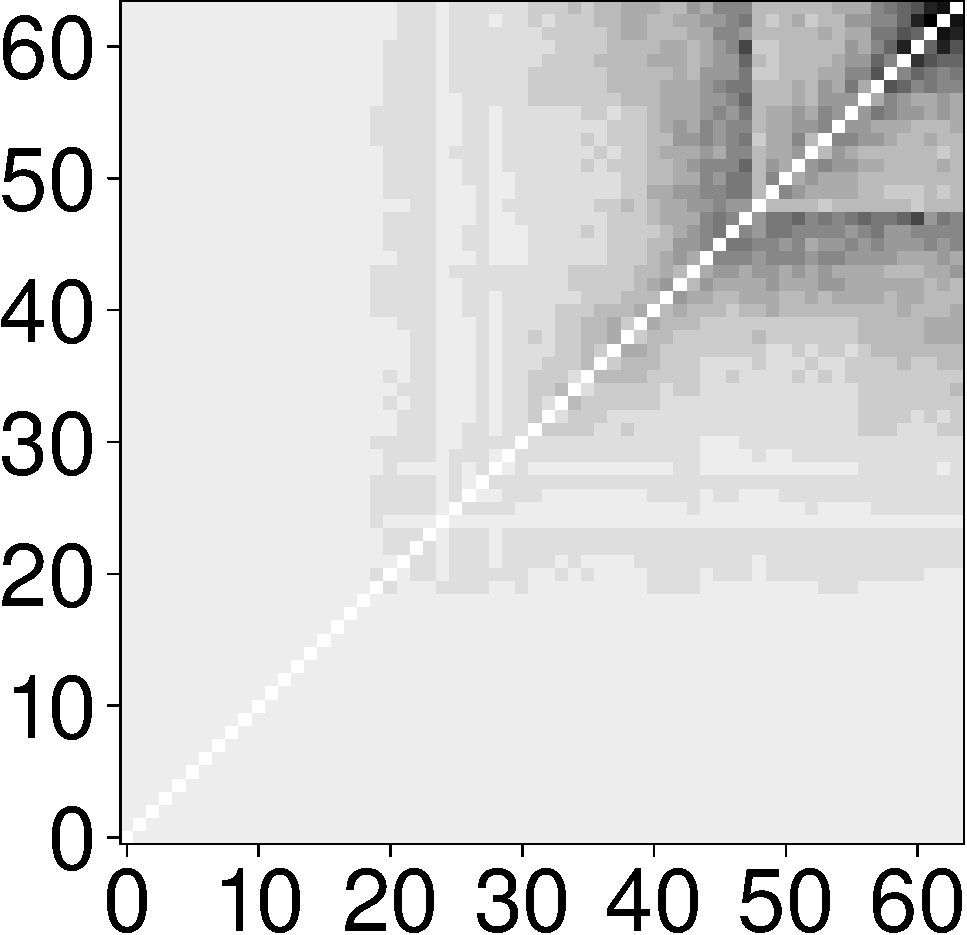
\includegraphics[width=\oneFPage\textwidth]{figures/mechanism/matrices/xeon/genome_64.pdf}
	}
	\subfigure[intruder]{
		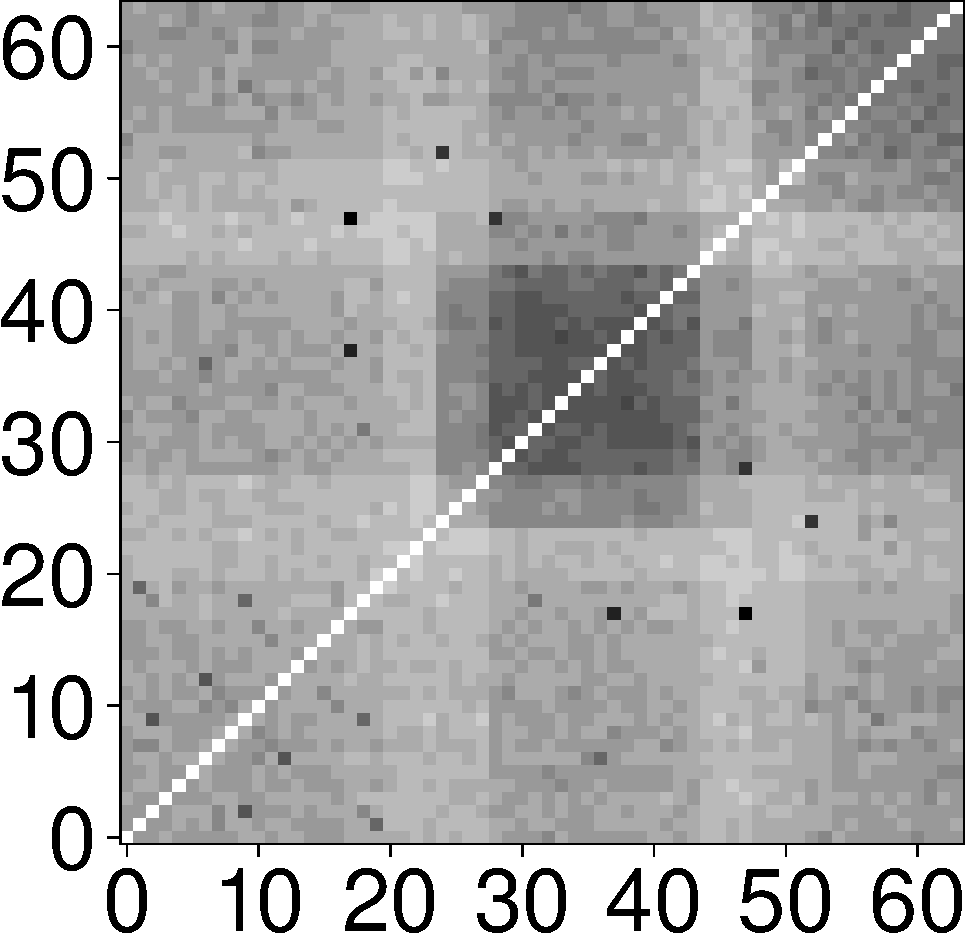
\includegraphics[width=\oneFPage\textwidth]{figures/mechanism/matrices/xeon/intruder_64.pdf}
	}
	\subfigure[kmeans]{
		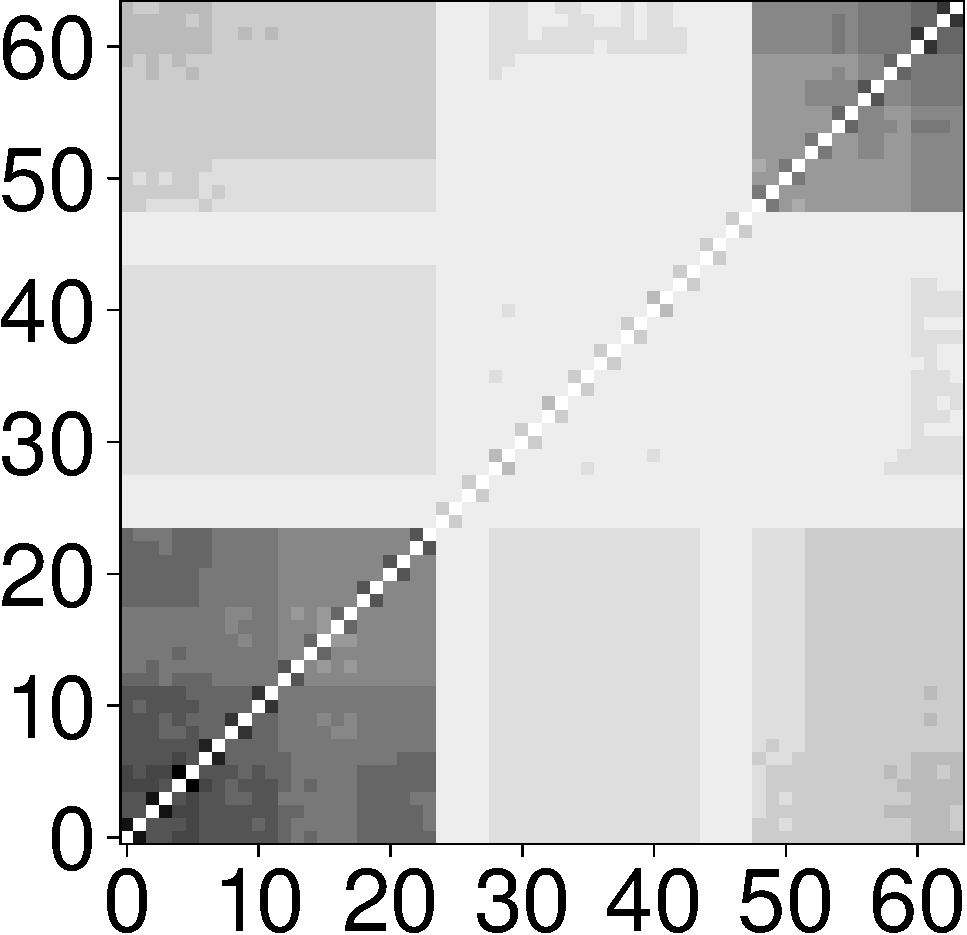
\includegraphics[width=\oneFPage\textwidth]{figures/mechanism/matrices/xeon/kmeans_64.pdf}
	}
	\subfigure[labyrinth]{
		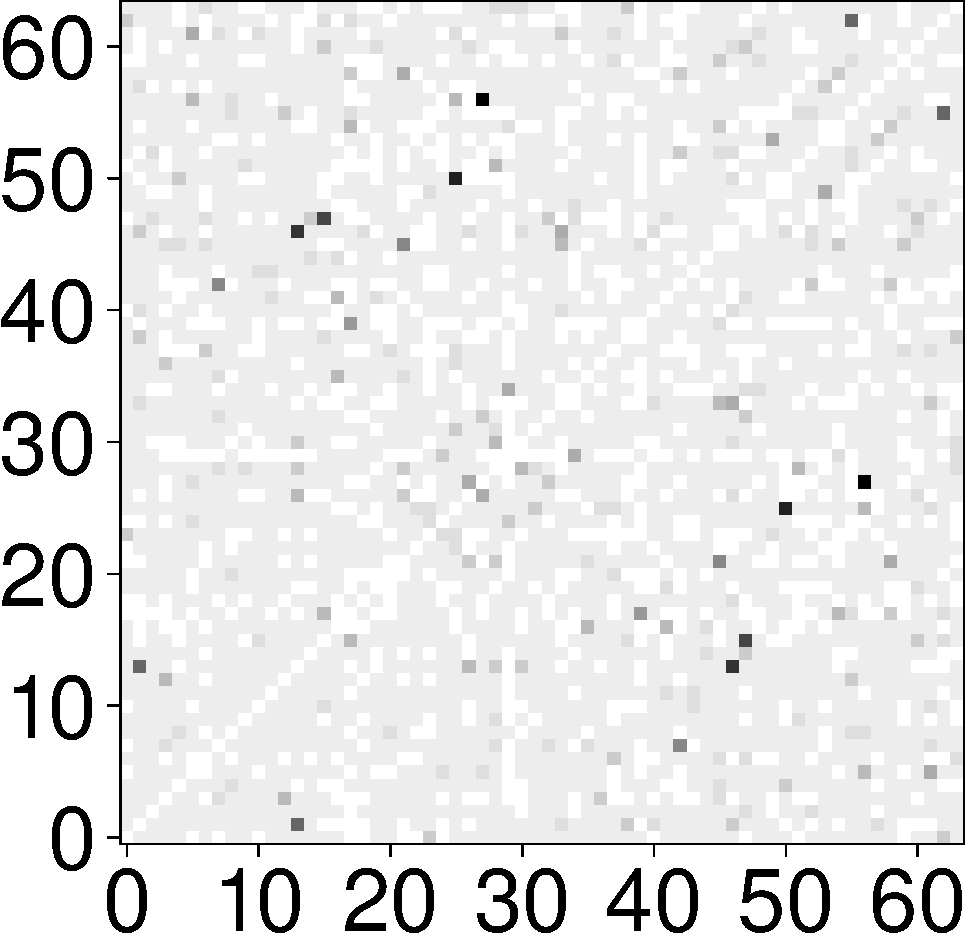
\includegraphics[width=\oneFPage\textwidth]{figures/mechanism/matrices/xeon/labyrinth_64.pdf}
	}
	\\
	\subfigure[ssca2]{
		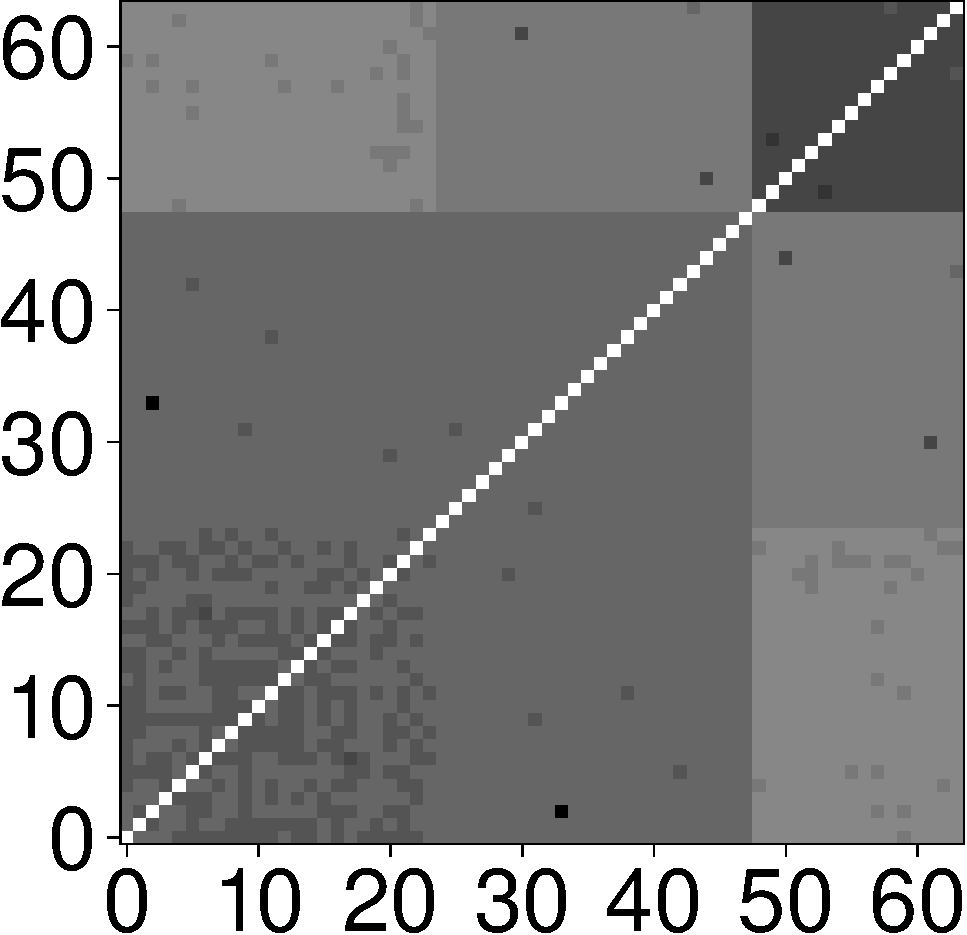
\includegraphics[width=\oneFPage\textwidth]{figures/mechanism/matrices/xeon/ssca2_64.pdf}
	}
	\subfigure[vacation]{
		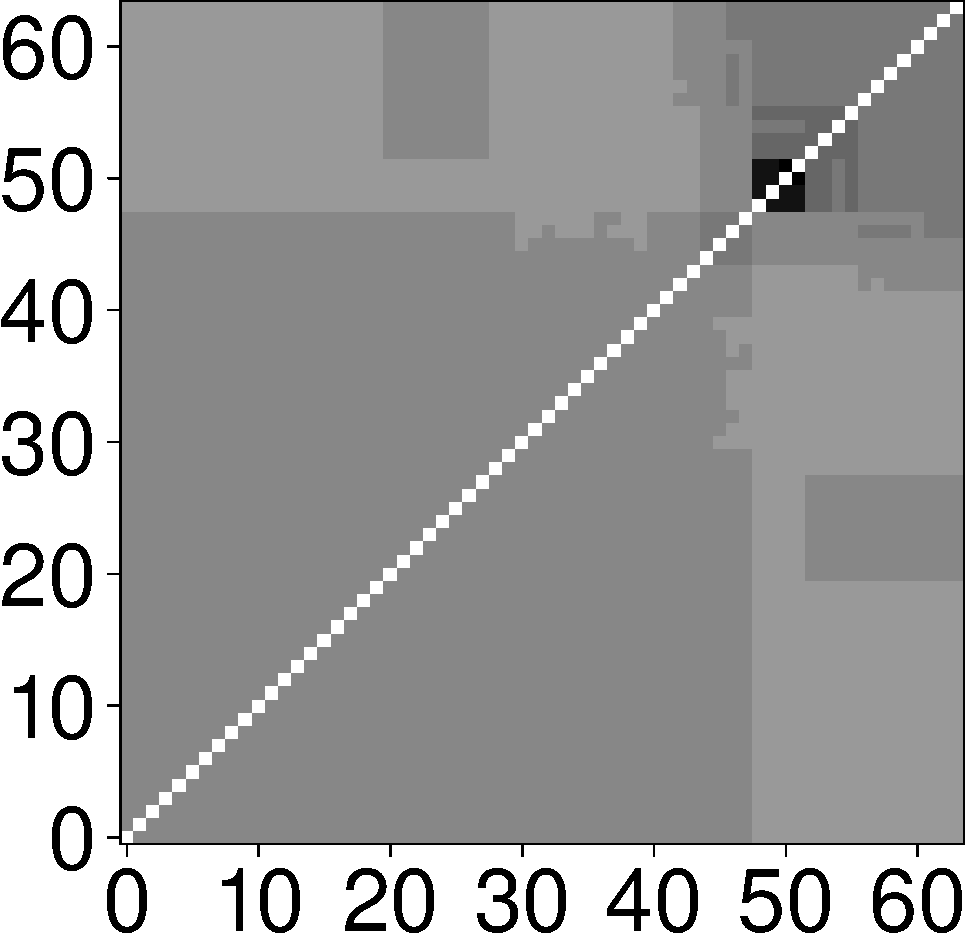
\includegraphics[width=\oneFPage\textwidth]{figures/mechanism/matrices/xeon/vacation_64.pdf}
	}
	\subfigure[yada]{
		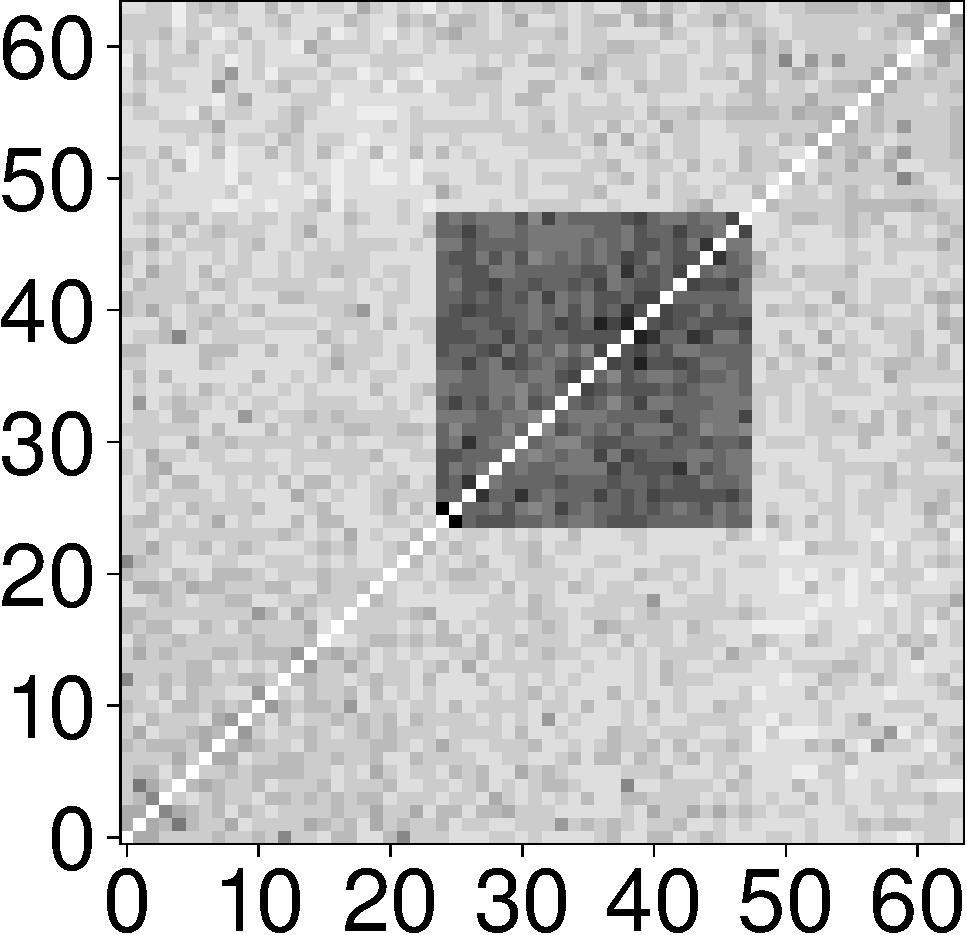
\includegraphics[width=\oneFPage\textwidth]{figures/mechanism/matrices/xeon/yada_64.pdf}
	}
	\subfigure[redblacktree]{
		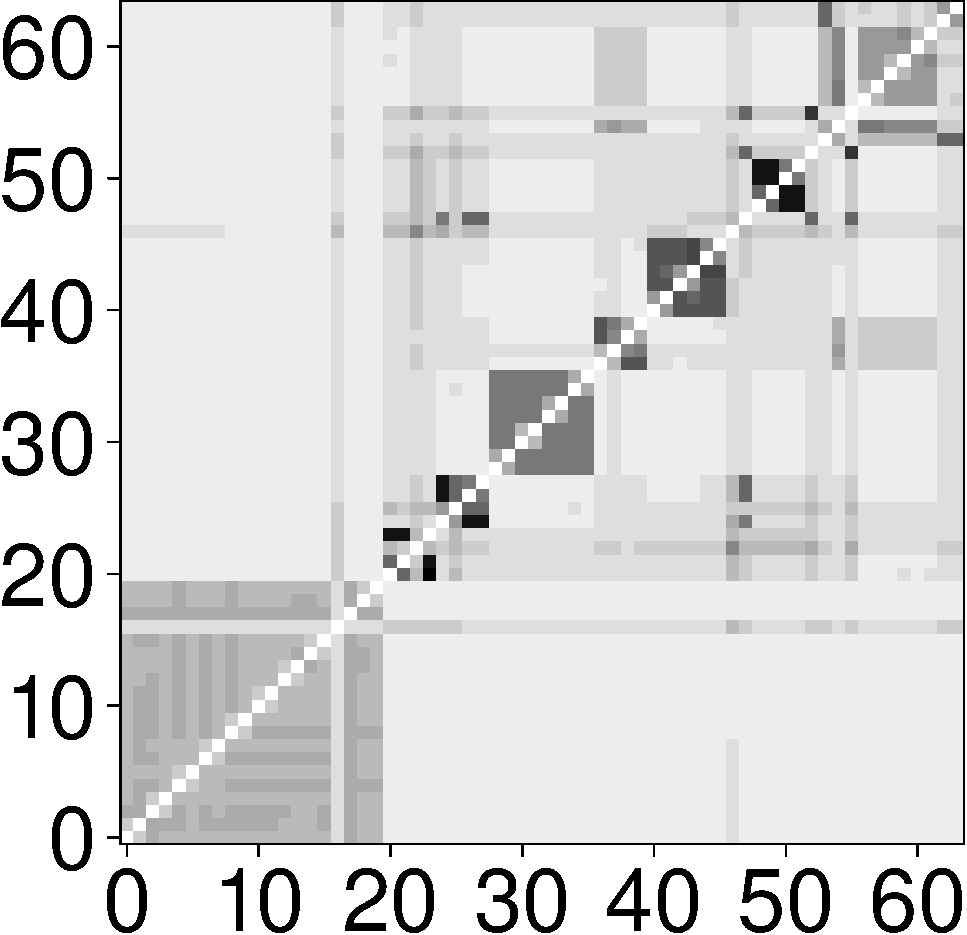
\includegraphics[width=\oneFPage\textwidth]{figures/mechanism/matrices/xeon/redblacktree_64.pdf}
	}
	\subfigure[hashmap]{
		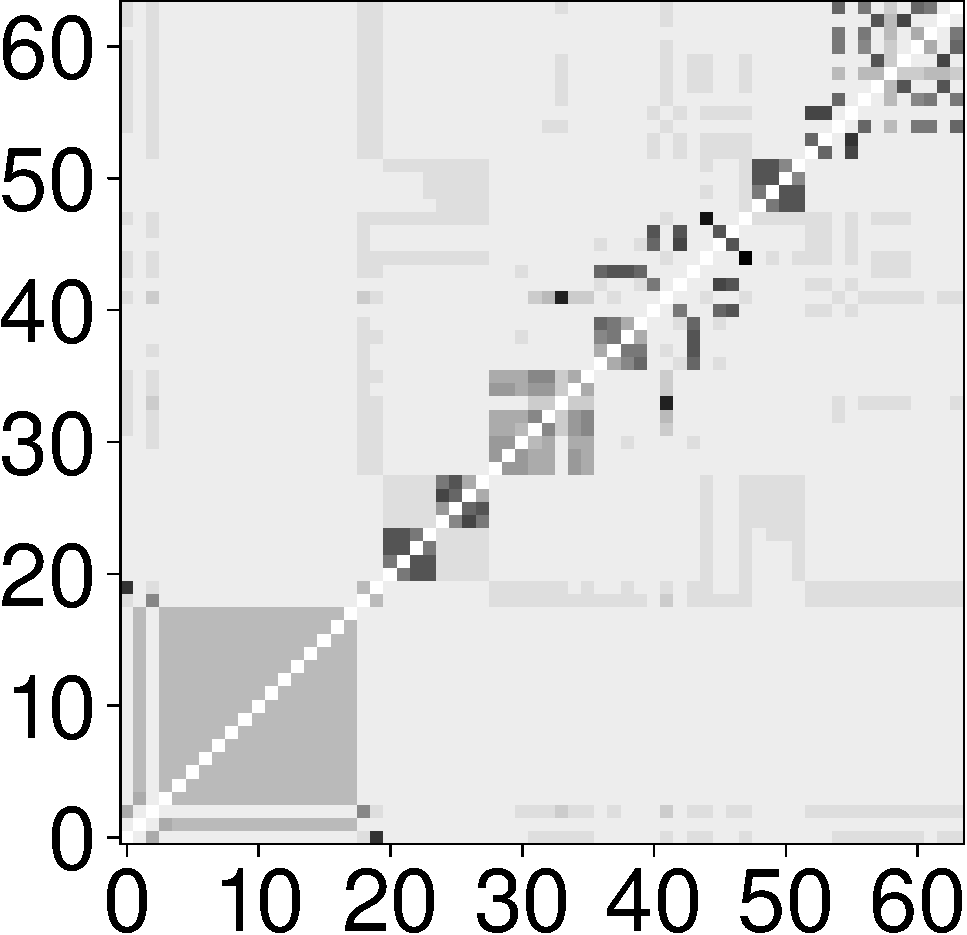
\includegraphics[width=\oneFPage\textwidth]{figures/mechanism/matrices/xeon/hashmap_64.pdf}
	}
	\caption{Communication matrices - 64 threads.}
\end{figure}

\begin{figure}[!tb]
	\centering
	\subfigure[bayes]{
		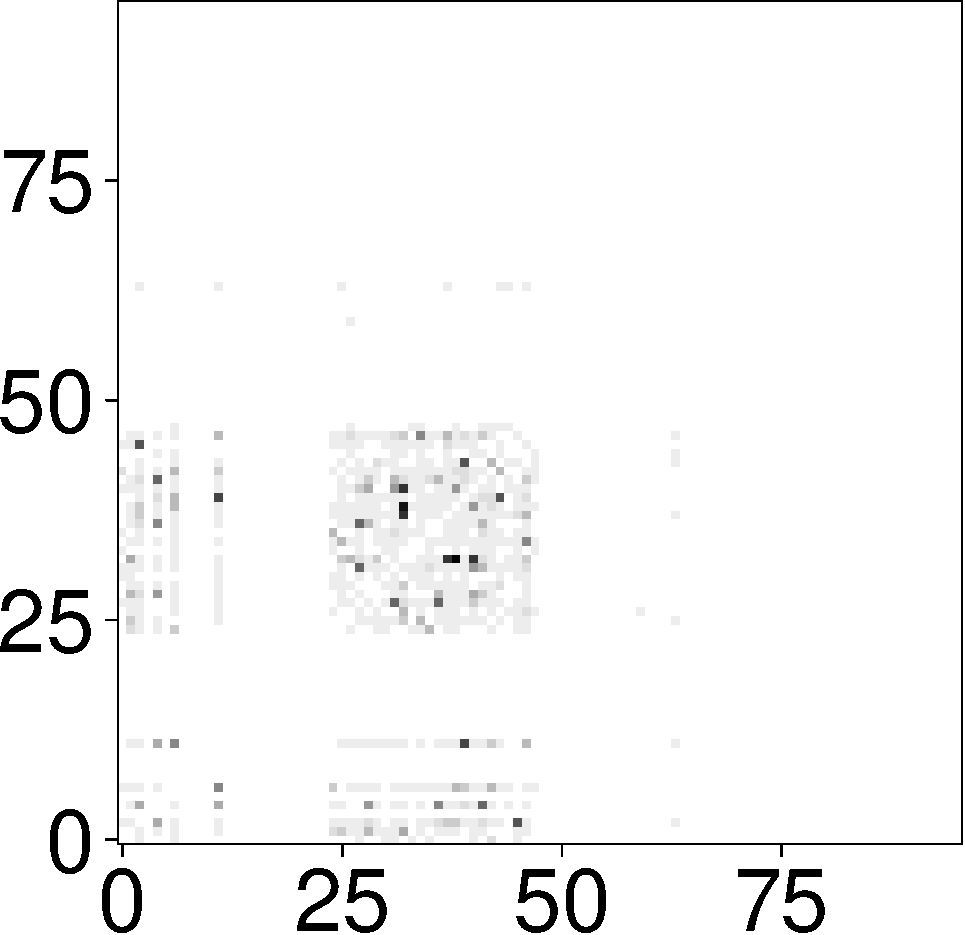
\includegraphics[width=\oneFPage\textwidth]{figures/mechanism/matrices/xeon/bayes_96.pdf}
	}
	\subfigure[genome]{
		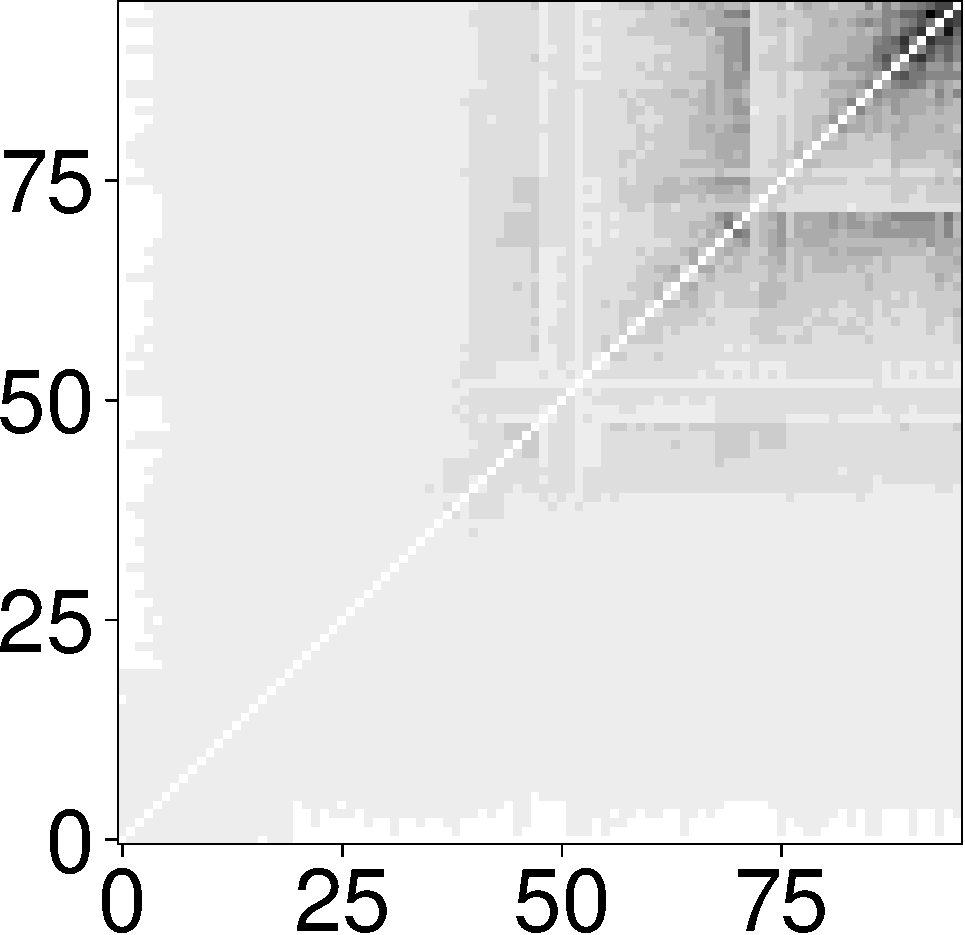
\includegraphics[width=\oneFPage\textwidth]{figures/mechanism/matrices/xeon/genome_96.pdf}
	}
	\subfigure[intruder]{
		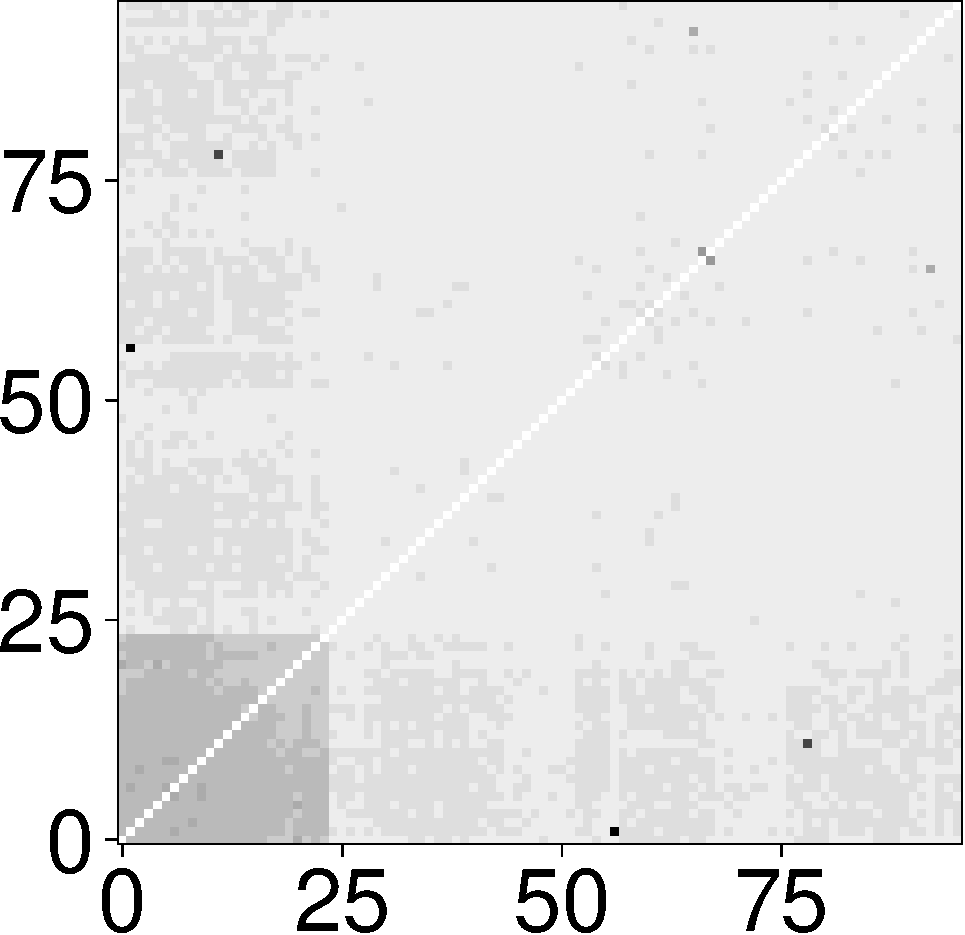
\includegraphics[width=\oneFPage\textwidth]{figures/mechanism/matrices/xeon/intruder_96.pdf}
	}
	\subfigure[kmeans]{
		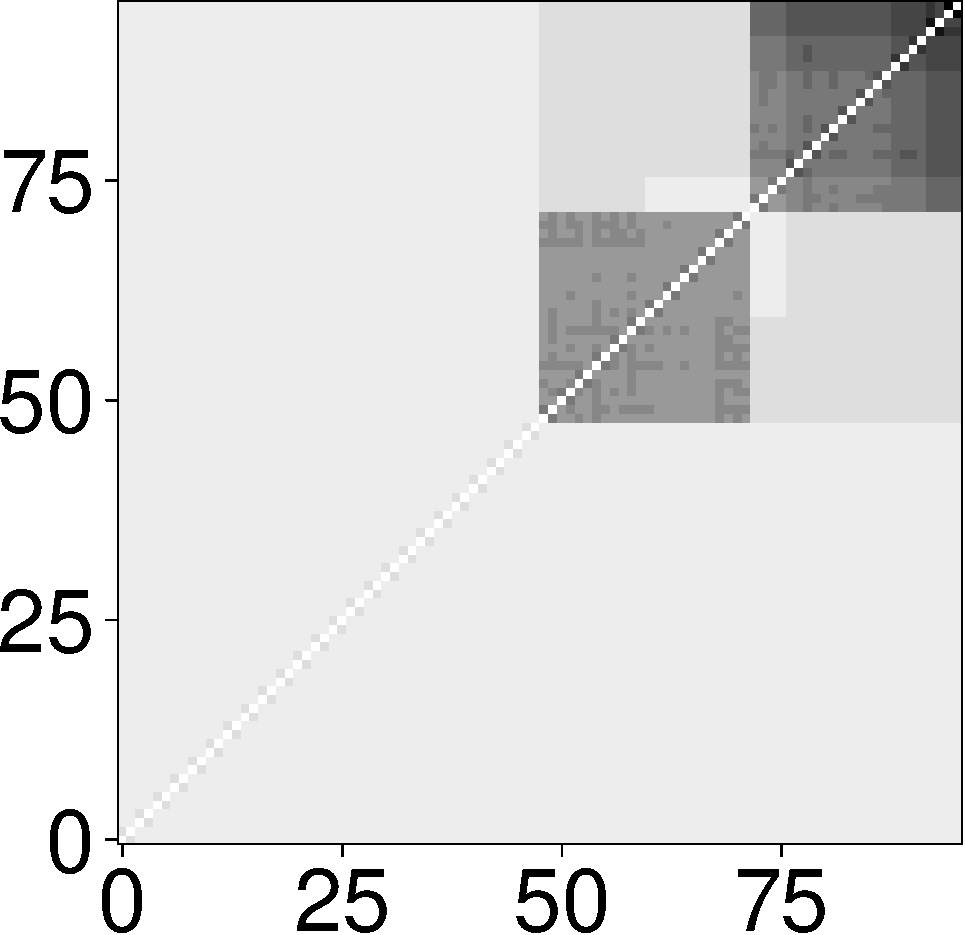
\includegraphics[width=\oneFPage\textwidth]{figures/mechanism/matrices/xeon/kmeans_96.pdf}
	}
	\subfigure[labyrinth]{
		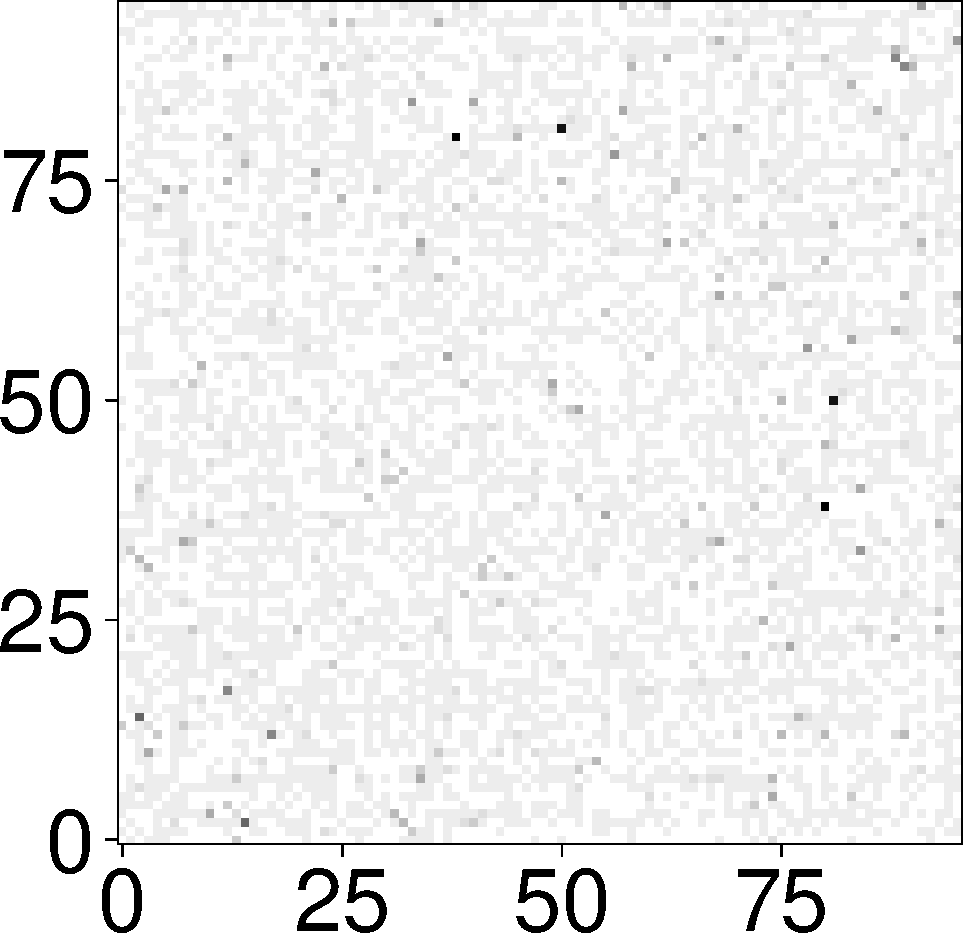
\includegraphics[width=\oneFPage\textwidth]{figures/mechanism/matrices/xeon/labyrinth_96.pdf}
	}
	\\
	\subfigure[ssca2]{
		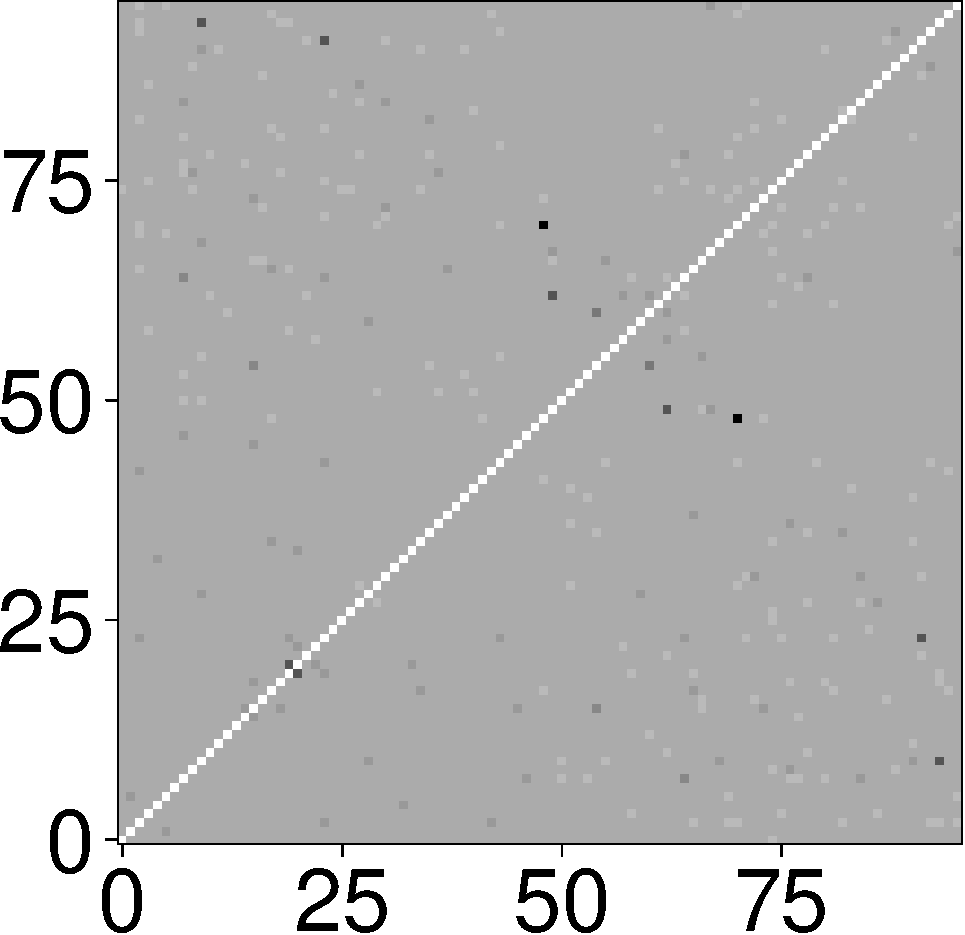
\includegraphics[width=\oneFPage\textwidth]{figures/mechanism/matrices/xeon/ssca2_96.pdf}
	}
	\subfigure[vacation]{
		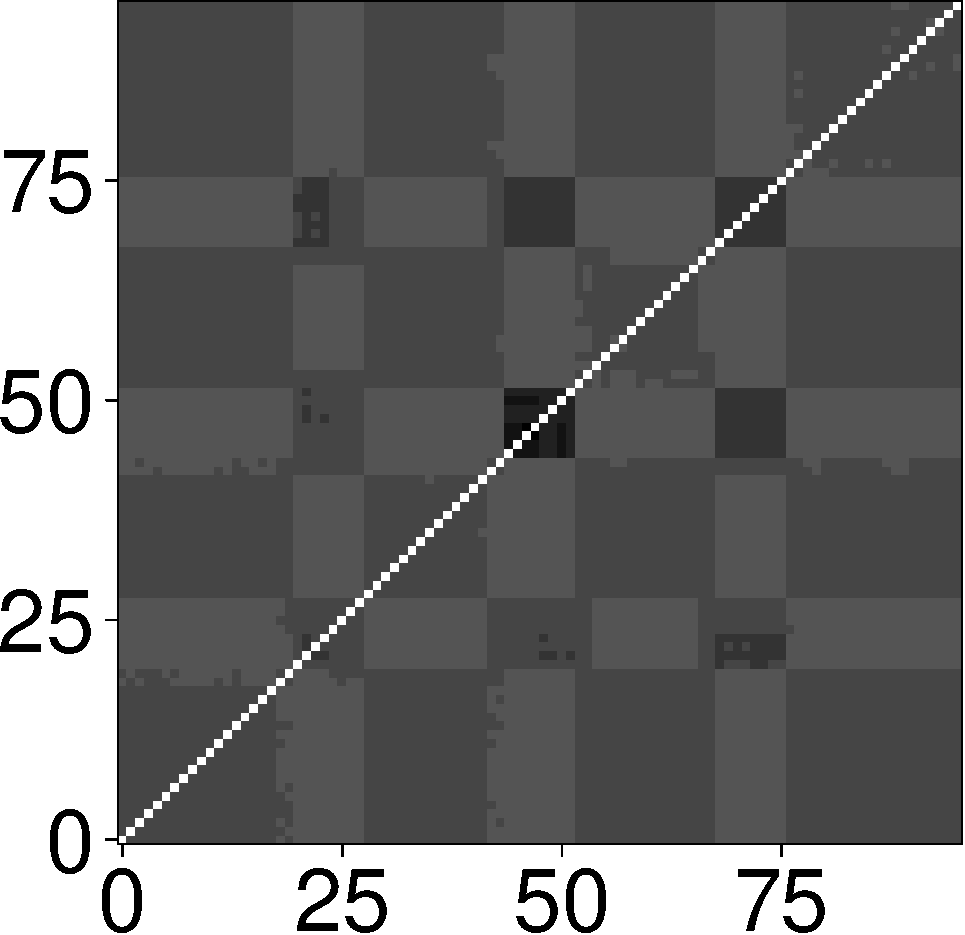
\includegraphics[width=\oneFPage\textwidth]{figures/mechanism/matrices/xeon/vacation_96.pdf}
	}
	\subfigure[yada]{
		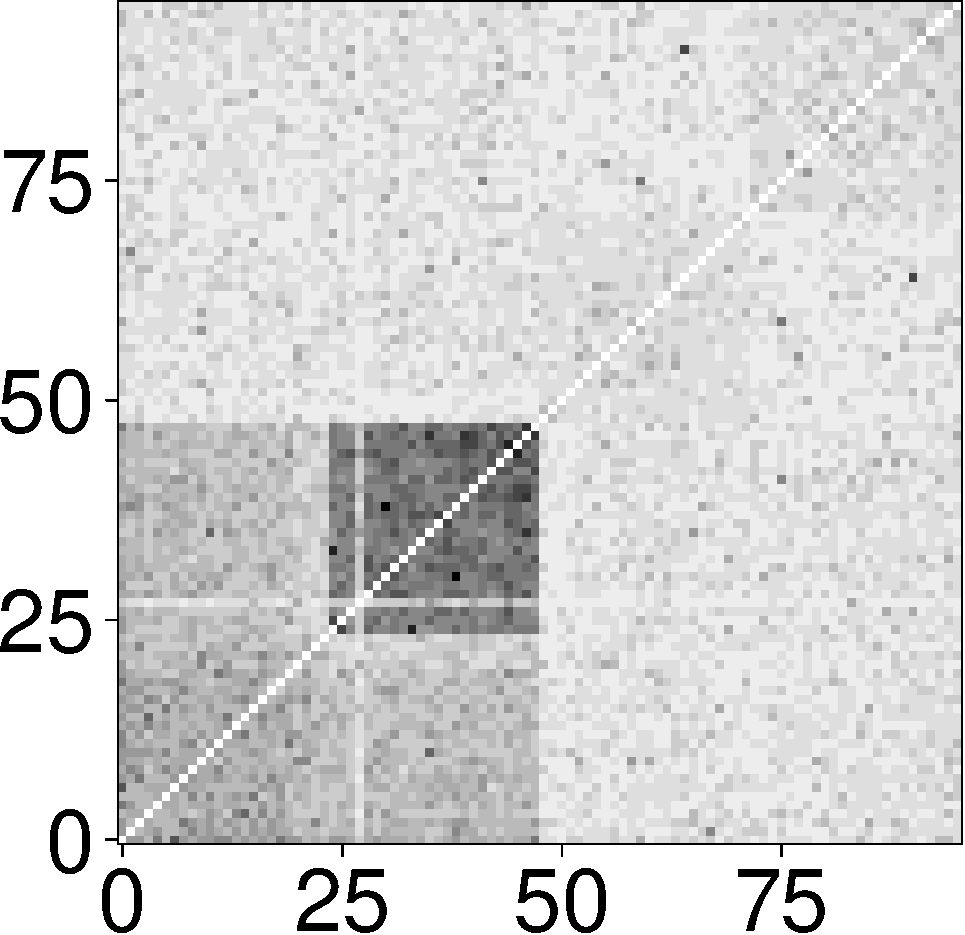
\includegraphics[width=\oneFPage\textwidth]{figures/mechanism/matrices/xeon/yada_96.pdf}
	}
	\subfigure[redblacktree]{
		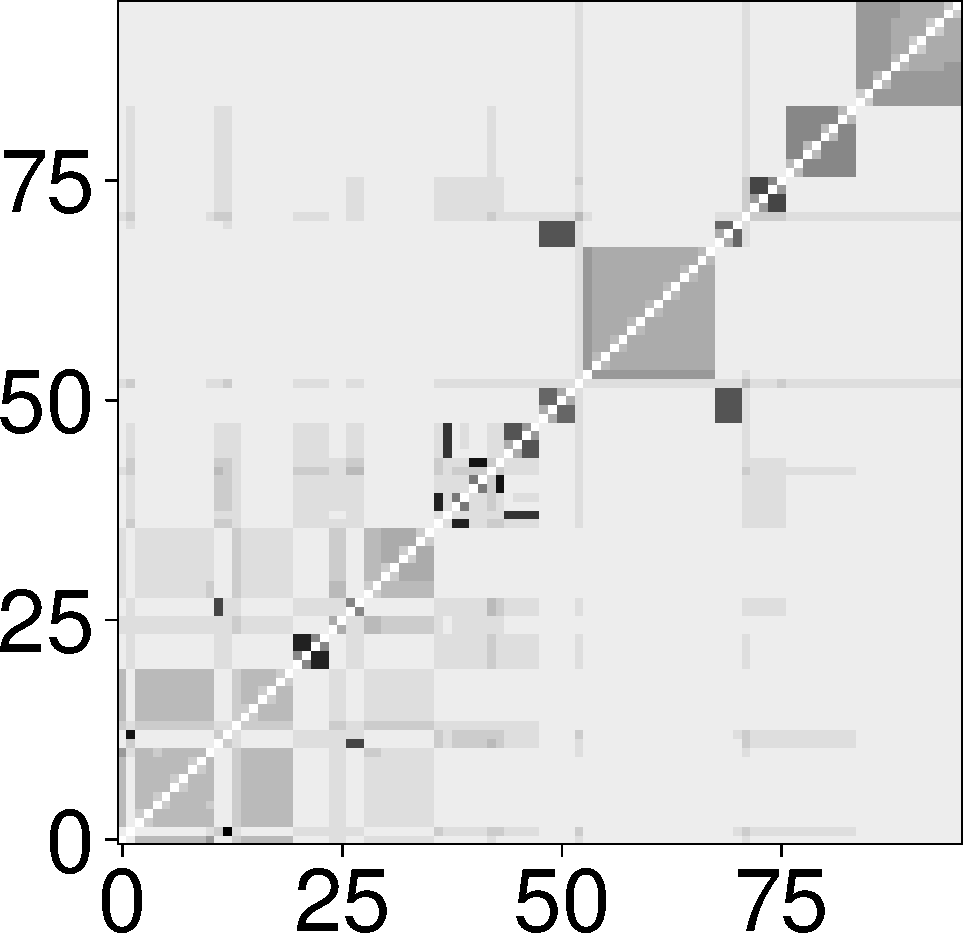
\includegraphics[width=\oneFPage\textwidth]{figures/mechanism/matrices/xeon/redblacktree_96.pdf}
	}
	\subfigure[hashmap]{
		\includegraphics[width=\oneFPage\textwidth]{figures/mechanism/matrices/xeon/hashmap_96.pdf}
	}
	\caption{Communication matrices - 96 threads.}
	\label{fig:commMatrXeon96}
\end{figure}



The two micro-benchmarks (HashMap and Redblacktree) present a communication pattern where neighbor threads communicate often. In that case, darker cells are localized closer to the main diagonal of the matrix. For this pattern, it is interesting to map threads on sibling cores to share all cache levels. On \emph{Genome}, only threads with higher IDs communicates often. Applications such as \emph{ssca2} and \emph{vacation} have an intense communication with all threads, know as all-to-all pattern~\cite{Williams:2009}. On the other hand, \emph{labyrinth} and \emph{bayes} present low communication intensity, but they are considered as an all-to-all pattern as well.


\subsection{Overhead}
To compare the overhead generated by tracking and generating the communication matrices, we compare our mechanism with a memory tracing tool called \texttt{numalize}~\cite{Diener2015}. For some applications \texttt{numalize} crashes and it is not possible the extract the communication matrix. This problem was also observed in others studies that have used this tool~\cite{Soomro:2018}: ``\textit{Unfortunately, in some cases, Numalize crashes because of the large memory requirements of an application in addition to its own internal data structures}''.
Hence, we were only able to run \emph{kmeans} using \texttt{numalize}.

\texttt{Numalize} depends on Intel's \texttt{Pin} tool~\cite{Luk:2005} to instrument the application and trace all accessed addresses, not only the ones accessed by the STM system. Therefore, \texttt{numalize} captures a different memory access behavior compared to our mechanism. This is visualized in \figurename~\ref{fig:numalizeCom} which compares the collected matrices of \emph{kmeans} with 32 and 64 threads using both mechanisms. %The MSE between the matrices collected by \texttt{numalize} and our mechanism is 824.72 (32 threads) and 524.97 (64 threads).

\begin{figure}[!ht]
	\centering
	\subfigure[numalize (32thr)]{
		\includegraphics[width=\oneQPage\textwidth]{figures/mechanism/NumalizeC/kmeans.full.6.comm.32.pdf}
	}
	\subfigure[our (32 threads)]{
		\includegraphics[width=\oneQPage\textwidth]{figures/mechanism/matrices/xeon/kmeans_32.pdf}
	}
	\subfigure[numalize (64thr)]{
		\includegraphics[width=\oneQPage\textwidth]{figures/mechanism/NumalizeC/kmeans.full.6.comm.pdf}
	}
	\subfigure[our (64 threads)]{
		\includegraphics[width=\oneQPage\textwidth]{figures/mechanism/matrices/xeon/kmeans_64.pdf}
	}
	\caption{Comparing \texttt{numalize} and our mechanism on \emph{kmeans}.}
	\label{fig:numalizeCom}
\end{figure}
Another disadvantage of \texttt{numalize} is the overhead added to trace all memory accesses. On \emph{kmeans}, using 64 threads, \texttt{numalize} took 690.90 seconds to execute the application and collect the communication matrix. By contrast, our mechanism took only 46.20 seconds for the same operation, almost 15$\times$ less. The normal execution time for \emph{kmeans} without tracing anything is 18.05 seconds, such that \texttt{numalize} added a overhead of 38.27$\times$, whereas the overhead was 2.5$\times$ with our mechanism. Although the overhead of our mechanism can be considered low, it is unfeasible to be used in an online mechanism. In Section~\ref{sec:lessoverhead}, we will show how to reduce this overhead to be able to perform the detection of sharing behavior during runtime.

%Use the graph of SBAC-PAD (sampling interval 0) to show the added overhead for each application, for collection the matrix.

\section{Summary}

This chapter presented a mechanism to detect the sharing behavior of STM applications. Since STM runtimes need the memory address on each data access operation and have precise information about shared variables, it is possible to determine the communication behavior by tracking transactional reads and writes instead of all memory accesses. Using the proposed mechanism it was possible to extract the sharing behavior of STM applications with lower overhead than other memory trace tools, such as \texttt{numalize}. Although the proposed mechanism has lower overhead, additional experiments are necessary to verify if the collected information is accurate, for instance, if they can be used to calculate an efficient thread mapping. These experiments will be made in Chapter~\ref{chap:sharAwareThreadMap}.

\chapter{Characterization of sharing-behavior of STM applications}\label{chap:charact}

For a successful thread mapping, it is necessary to perform an in-depth analysis of STM applications, for instance, if the memory access pattern changes in each execution; the number of addresses accessed inside transactions, etc. This analysis is important to guide decisions regarding mapping, such as determining if an application is suitable for a thread mapping based on communication behavior and defining the type of mapping policy (static or dynamic). %In the context of this paper, communication and sharing are used interchangeably and have the same meaning.

In this chapter, we characterize the applications from \texttt{STAMP}~\cite{STAMP}, by gathering sharing information through the proposed mechanism in Chapter~\ref{chap:mechanism}, providing information to guide thread placement based on their sharing behavior. The \texttt{STAMP} benchmark was developed with the intention to represent realistic workload characteristics and different application domains. Besides, \texttt{STAMP} covers a wide range of transactional behavior, for instance, varying transaction lengths, contention, quantity of transactions, etc. Hence, we expect that the characterization done in this chapter could represent a wide range of real STM applications. Using the proposed mechanism we are able to gather information about the suitability for thread mapping of each application, its communication pattern, and its dynamic behavior, among others. We also show how this mechanism can be used to detect false sharing of cache lines of STM operations.


\section{Methodology of the Characterization}\label{sec:methodology}
%This section discusses the methodology of the characterization.

\subsection{Detecting sharing in STM applications}
The characteristics of memory access behavior presented in this thesis are based on the communication matrices of applications. To extract the matrices we have used the mechanism proposed in Chapter~\ref{chap:mechanism}. %This mechanism is triggered on each transactional data access operation (read or write). When at least two different threads accessed the same memory address, a communication event between them is stored in a communication matrix. Examples of communication matrices are shown in Fig.~\ref{fig:FirstQMatrices}. Axes show threads IDs. The mechanism was implemented in the \texttt{TinySTM} library~\cite{TinySTM2}, version 1.0.5. \texttt{TinySTM} was configured to use the default configuration: \emph{lazy} version management, \emph{eager} conflict detection and contention manager \emph{suicide}.
%
\texttt{STAMP} was compiled with gcc~8.3.0. If not specified otherwise, all applications were executed ten times using 64 threads and the default input parameters shown in \tablename~\ref{tab:defaultParams}. We also used the same Xeon machine described on Section~\ref{sec:mechMethodology} to run the experiments.
 %, where \thNumber~represents the number of threads. 
%Most parameters are larger than the largest ones suggested in the original paper~\cite{STAMP} to achieve more substantial execution times on modern machines. %\new{The idea to change it was to make each application run for at least ten seconds.}

%\begin{table}[!tb]
%	\small
%	\centering
%	\caption{Default arguments for the programs used in the experiments.}
%	\label{tab:defaultParams}
%	\begin{tabular}{@{}ll@{}}
%		\toprule
%		Application & Arguments                                          \\ \midrule
%		bayes                & \texttt{-v32 -r8192 -n10 -p40 -i2 -e8 -s1 -t \thNumber}                \\
%		genome               & \texttt{-g49152 -s256 -n33554432 -t \thNumber}                         \\
%		intruder             & \texttt{-a10 -l128 -n262144 -s1 -t \thNumber}                          \\
%		kmeans               & \texttt{-m40 -n40 -t0.00001 -i random-n65536-d32-c16.txt -p \thNumber}\\
%		labyrinth            & \texttt{-i random-x1024-y1024-z9-n1024.txt -t \thNumber}               \\
%		ssca2                & \texttt{-s21 -i1.0 -u1.0 -l3 -p3 -t \thNumber}                         \\
%		vacation             & \texttt{-n4 -q90 -u100 -r1310720 -t16777216 -c \thNumber}              \\
%		yada                 & \texttt{-a15 -i ttimeu1000000.2 -t \thNumber}                          \\
%		\bottomrule
%	\end{tabular}
%\end{table}
%\subsection{Machine}

%Applications were executed on an eight-socket Intel Xeon E5-4650 system, running Linux kernel 4.19.0-9. Each socket has 12 2-HT cores, totaling 96 cores. Each socket corresponds to a NUMA node (for a total of 8 NUMA nodes), and 12$\times$ 32 KB L1d, 12$\times$ 32 KB L1i, 12$\times$ 256 KB L2 and 30 MB L3 caches.

\subsection{Mean squared error (MSE)}\label{sec:MSE}

Since the analysis of the communication behavior of the applications is based on communication matrices, we used \emph{Mean squared error} (MSE)~\cite{MSE} metric to compare the difference between them, which has been used in prior work for this purpose~\cite{Diener:2016:2}. The equation to calculate the MSE is shown in Eq.~\ref{eq:MSE}.

\begin{samepage}
	\begin{equation}
		MSE(A, B) =  \frac{1}{N^2}\sum_{i=0}^{N-1}\sum_{j=0}^{N-1}(A[i,j]-B[i,j])^2
		\label{eq:MSE}
	\end{equation}
	where:
	\begin{conditions}
		A, B     &  input matrices \\
		N        &  matrix order, i.e., number of threads \\
		i,j      &  matrix indexes
	\end{conditions}
\end{samepage}

If the MSE of two matrices is zero, then the matrices are exactly the same. Higher MSE values indicate higher differences. This metric is useful to compare, for instance, if the memory access behavior of one application changes on each execution. %In that case, values closer to zero indicate that the matrices are more similar.

\subsection{Experiments}\label{sec:experiments}

We performed the following experiments to characterize the sharing behavior of the \texttt{STAMP} applications:

\begin{enumerate}
	\item We collected information about the total of accessed addresses inside the STM library. The information is useful to understand how much data is accessed by STM operations (Section~\ref{sec:falseSharing}).
	
	\item We executed the same application ten times to verify if the communication pattern changes between executions. This experiment will show if a communication matrix collected in a previous execution can be used to make a static thread mapping (Section~\ref{sec:sameDIffExecs}).
	
	\item We executed the same application ten times, changing the input parameters from the default. This experiment will show if it is possible to use a collected communication matrix with different input parameters to make a static thread mapping (Section~\ref{sec:newInput}).
	
	\item We executed the same application ten times, changing the total number of threads from the previous experiments, with the same goal as in the previous item (Section~\ref{sec:differentThreads}).
	
	\item We collected the communication matrix several times during the execution of an application, to determine if an application needs an online mechanism to detect the sharing behavior and perform the thread mapping multiple times during execution (Section~\ref{sec:dynamicBehavior}).
\end{enumerate}

\section{Characterization of sharing behavior}\label{sec:charact}

This section presents the characterization of the \texttt{STAMP} applications, regarding memory access behavior.

\subsection{STM memory access information}\label{sec:falseSharing}

The first data set is not directly related to sharing behavior but is useful to explain further the behavior of applications.
The total number of distinct memory addresses accessed by STM operations was collected as well as the total number of accesses made to these addresses such as read or write operations. With this data, it is possible to calculate other information:
\begin{itemize}
	\item \textbf{Number of distinct cache lines}: This was calculated based on the default cache line of most current microarchitectures, 64 bytes.
	
	\item \textbf{Number of distinct pages}: This was calculated based on the default page size of many current microarchitectures, 4096 bytes.
	
	\item \textbf{Percentage of cache lines with false sharing}: We consider that a cache line has false sharing when multiple threads perform STM operations on more than one word at the same line.
\end{itemize}

\begin{table}[ht]
	\centering
	\caption{Analysis of accessed STM memory addresses in STAMP applications.}
	\label{tab:falseSharing}
\begin{tabular}{l@{\hspace*{10pt}}r@{\hspace*{10pt}}r@{\hspace*{10pt}}r@{\hspace*{10pt}}r@{\hspace*{10pt}}r}
	\toprule
	{Application} & \multicolumn{1}{c}{{\begin{tabular}[c]{r}Distinct \\ addresses\end{tabular}}} & \multicolumn{1}{c}{{\begin{tabular}[c]{@{}r@{}}Distinct \\ cache lines\end{tabular}}} & \multicolumn{1}{c}{{\begin{tabular}[c]{@{}r@{}}Distinct \\ pages\end{tabular}}} & \multicolumn{1}{c}{{\begin{tabular}[c]{@{}r@{}}Total \\ accesses\end{tabular}}} & \multicolumn{1}{c}{{\begin{tabular}[c]{@{}r@{}}\% of lines with  \\ false  sharing\end{tabular}}} \\ \midrule
	bayes                & 1,082                                                                                      & 497                                                                                         & 122                                                                                     & 15,928,303                                                                             & 89.33                                                                                    \\
	kmeans               & 682                                                                                        & 101                                                                                         & 4                                                                                      & 833,954,131                                                                            & 100.00                                                                                   \\
	labyrinth            & 824,126                                                                                    & 290,083                                                                                     & 18,213                                                                                 & 1,994,315                                                                              & 83.05                                                                                    \\
	genome               & 19,750,104                                                                                 & 11,216,870                                                                                  & 452,651                                                                                & 2,840,508,725                                                                          & 36.21                                                                                    \\
	intruder             & 23,292,164                                                                                 & 8,131,906                                                                                   & 297,629                                                                                & 4,105,619,590                                                                          & 99.00                                                                                    \\
	yada                 & 25,055,077                                                                                 & 13,932,226                                                                                  & 848,045                                                                                & 610,446,722                                                                            & 81.38                                                                                    \\
	vacation             & 33,671,744                                                                                 & 10,796,118                                                                                  & 799,129                                                                                & 7,212,365,036                                                                          & 99.08                                                                                    \\
	ssca2                & 91,335,091                                                                                 & 13,907,852                                                                                  & 528,387                                                                                & 270,369,505                                                                            & 99.90                                                                                    \\ \bottomrule
\end{tabular}
\end{table}

Results are shown in \tablename~\ref{tab:falseSharing} and indicate that the applications have different characteristics regarding the number of accessed addresses. \textit{kmeans} has the lowest amount of distinct addresses accessed. However, it has a large number of total accesses made to these addresses. On the other hand, \textit{ssca2} has the largest amount of distinct addresses accessed, but not the largest total of accesses, which belongs to \textit{vacation}.
%
Regarding false sharing, the majority of applications have a large percentage of false sharing. For instance, in \textit{kmeans}, all addresses share common cache lines. On the other hand, \textit{genome} has the least amount of false sharing which indicates that more than half of the accessed addresses has at least 64 bytes or the addresses that conflict in the same cache line are accessed outside the STM library.

\subsection{Stability of sharing behavior across different executions}\label{sec:sameDIffExecs}

The goal of this experiment is to determine if the communication pattern changes across different executions of the same application, using the same input parameters and number of threads. To answer this question, we executed all applications one time and collected the communication matrix, to be used as a baseline for comparison. After that, we run each application nine more times, collecting the communication matrix in each execution. Then, we calculated the MSE of each resulting matrix, comparing it to the first execution. Results are shown in~\figurename~\ref{fig:averageFirstQ}.

\begin{figure}[!t]
	\centering
	\includegraphics[width=\fullImageWidth\textwidth]{figures/sharingBehavior/FirstQ/0.graph.pdf}
	\caption{Stability of the sharing behavior across different executions.}
	\label{fig:averageFirstQ}
\end{figure}

Some applications, for instance \emph{bayes}, \emph{genome} and \emph{labyrinth}, present the same communication behavior in all executions. This observation can be visualized in two different communication matrices of \emph{bayes} (\figurename~\ref{fig:FirstQBayes1} and \figurename~\ref{fig:FirstQBayes2}). Axes show threads IDs.
\begin{figure}[!t]
	\centering
	\subfigure[bayes]{
		\includegraphics[width=\oneQPage\textwidth]{figures/sharingBehavior/FirstQ/bayes_64.pdf}
		\label{fig:FirstQBayes1}
	}
	\subfigure[bayes]{
		\includegraphics[width=\oneQPage\textwidth]{figures/sharingBehavior/FirstQ/bayes_64_5.pdf}
		\label{fig:FirstQBayes2}
	}
	\subfigure[ssca2]{
		\includegraphics[width=\oneQPage\textwidth]{figures/sharingBehavior/FirstQ/ssca2_64.pdf}
		\label{fig:FirstQssca21}
	}
	\subfigure[ssca2]{
		\includegraphics[width=\oneQPage\textwidth]{figures/sharingBehavior/FirstQ/ssca2_64_7.pdf}
		\label{fig:FirstQssca22}
	}
	\caption{Matrices with highest and lowest MSEs between different executions.}
	\label{fig:FirstQMatrices}
\end{figure}
In contrast to \emph{bayes}, \emph{ssca2} presents a not so similar behavior on each execution. However, looking at two \emph{ssca2} matrices (\figurename~\ref{fig:FirstQssca21}) and \figurename~\ref{fig:FirstQssca22}) it is possible to note that although the basic communication behavior is the same (all-to-all \cite{Williams:2009}), the total amount of communication between threads is very different. This can be explained by  the non-deterministic behavior of TM applications, mainly due to the fact that the total number of aborts varies in each execution. More aborts imply in more work to be done, consequently more communication between threads. In that case, even having a higher MSE between executions, \emph{ssca2} has a similar behavior of communication between threads (all-to-all pattern) in all executions.

\subsection{Stability of sharing behavior when changing input parameters}\label{sec:newInput}

For this experiment, instead of using the default input parameters shown in \tablename~\ref{tab:defaultParams}, we used a smaller input data set. The changed parameters are shown in \tablename~\ref{tab:changedParams}.
\begin{table}[!ht]
	\centering
	\caption{Small input parameters used in the experiments in Section~\ref{sec:newInput}.}
	\label{tab:changedParams}
	\begin{tabularx}{\textwidth}{@{}lXl@{}}
	\toprule
	Application & Arguments                                          \\ \midrule
	bayes                & \texttt{-v16 -r4096 -n15 -p40 -i2 -e8 -s1 -t \thNumber}                \\
	genome               & \texttt{-g16384 -s64 -n16777216 -t \thNumber}                         \\
	intruder             & \texttt{-a10 -l64 -n131072 -s1 -t \thNumber}                          \\
	kmeans               & \texttt{-m15 -n15 -t0.00001 -i random-n65536-d32-c16.txt -p \thNumber}\\
	labyrinth            & \texttt{-i random-x512-y512-z7-n512.txt -t \thNumber}               \\
	ssca2                & \texttt{-s18 -i1.0 -u1.0 -l3 -p3 -t \thNumber}                         \\
	vacation             & \texttt{-n4 -q60 -u90 -r1048576 -t4194304 -c \thNumber}              \\
	yada                 & \texttt{-a20 -i ttimeu100000.2 -t \thNumber}                          \\
	\bottomrule
\end{tabularx}
\end{table}
Then, we collected ten communication matrices using the same methodology of Section~\ref{sec:sameDIffExecs}. Lastly, a comparison of the MSE using the default parameters (Section~\ref{sec:sameDIffExecs}) was made, comparing with the small parameters (\tablename~\ref{tab:changedParams}). This comparison is shown in \figurename~\ref{fig:averageSecondQ}.

\begin{figure}[!tb]
	\centering
	\includegraphics[width=\fullImageWidth\textwidth]{figures/sharingBehavior/SecondQ/0.graph.pdf}
	\caption{Stability of the sharing behavior when changing input parameters.}
	\label{fig:averageSecondQ}
\end{figure}

As in the previous experiment, \emph{ssca2} has a different pattern on each execution. For instance, \figurename~\ref{fig:SecondQssca21} and
\figurename~\ref{fig:SecondQssca22} show two different executions of  \emph{ssca2}, using the small parameters (\tablename~\ref{tab:changedParams}).
\begin{figure}[!tb]
	\centering
	\subfigure[genome-default]{
		\includegraphics[width=\oneQPage\textwidth]{figures/sharingBehavior/SecondQ/genome_64_2-Default.pdf}
		\label{fig:SecondQgenomeD}
	}
	\subfigure[genome-small]{
		\includegraphics[width=\oneQPage\textwidth]{figures/sharingBehavior/SecondQ/genome_64_3-Changed.pdf}
		\label{fig:SecondQgenomeC}
	}
	\subfigure[ssca2-small]{
		\includegraphics[width=\oneQPage\textwidth]{figures/sharingBehavior/SecondQ/ssca2_64.pdf}
		\label{fig:SecondQssca21}
	}
	\subfigure[ssca2-small]{
		\includegraphics[width=\oneQPage\textwidth]{figures/sharingBehavior/SecondQ/ssca2_64_8.pdf}
		\label{fig:SecondQssca22}
	}
	\caption{Matrices with highest and lowest MSEs.}
	\label{fig:SecondQMatrices}
\end{figure}
However, with the new parameters, it is possible to observe that some groups of threads communicate more often than others (\figurename~\ref{fig:SecondQssca21}). Besides, there is a difference between communication patterns taking into consideration the default and small parameter sets. This can be visualized by comparing \figurename~\ref{fig:FirstQssca21} and \figurename~\ref{fig:SecondQssca21}. Other applications such as \emph{intruder}, \emph{kmeans}, and \emph{vacation} have a small difference between communication patterns when changing input parameters. While others, such as \emph{genome} have almost the same communication pattern, even when changing the input parameters (\figurename~\ref{fig:SecondQgenomeD} and \figurename~\ref{fig:SecondQgenomeC}).

\subsection{Stability of sharing behavior with different numbers of threads}\label{sec:differentThreads}

\figurename~\ref{fig:averageFirstQ} in Section~\ref{sec:sameDIffExecs} showed the communication matrices for 64 threads. We used the same methodology to collect them for 32 and 96 threads, and show the results in \figurename~\ref{fig:averageThirdQ}.
%
\begin{figure}[!t]
	\centering
	\subfigure[32 threads.]{
		\includegraphics[width=\halfPage\textwidth]{figures/sharingBehavior/ThirdQ/Default32Threads.pdf}
		\label{fig:ThirdQ32Threads}
	}
	\subfigure[96 threads.]{
		\includegraphics[width=\halfPage\textwidth]{figures/sharingBehavior/ThirdQ/Default96Threads.pdf}
		\label{fig:ThirdQ96Threads}
	}
	\caption{Stability of the sharing behavior when changing the number of threads.}
	\label{fig:averageThirdQ}
\end{figure}
%
The most different behavior occurs with \emph{vacation} and 96 threads. However, looking at the communication pattern of two executions with the highest MSE (\figurename~\ref{fig:ThirdQvacation961} and \figurename~\ref{fig:ThirdQvacation962}) we saw the same behavior for \emph{ssca2} in Section~\ref{sec:sameDIffExecs}.
\begin{figure}[!ht]
	\centering
	\subfigure[genome (32 thr)]{
		\includegraphics[width=\oneQPage\textwidth]{figures/sharingBehavior/ThirdQ/genome_32.pdf}
		\label{fig:ThirdQgenome321}
	}
	\subfigure[genome (32 thr)]{
		\includegraphics[width=\oneQPage\textwidth]{figures/sharingBehavior/ThirdQ/genome_32_1.pdf}
		\label{fig:ThirdQgenome322}
	}
	\subfigure[vacation (96 thr)]{
		\includegraphics[width=\oneQPage\textwidth]{figures/sharingBehavior/ThirdQ/vacation_96.pdf}
		\label{fig:ThirdQvacation961}
	}
	\subfigure[vacation (96 thr)]{
		\includegraphics[width=\oneQPage\textwidth]{figures/sharingBehavior/ThirdQ/vacation_96_5.pdf}
		\label{fig:ThirdQvacation962}
	}
	\caption{Matrices with the lowest and highest MSEs.}
	\label{fig:ThirdQMatrices}
\end{figure}
With 96 threads, \emph{vacation} has an all-to-all communication pattern, and the main difference between executions is the total amount of communication, which can be explained by the difference of aborts between each execution. On the other hand, applications such as \emph{genome} present a similar behavior even changing the number of threads, for instance, with 32 threads (\figurename~\ref{fig:ThirdQgenome321} and \figurename~\ref{fig:ThirdQgenome322}).


\subsection{Dynamic behavior during execution}\label{sec:dynamicBehavior}

The goal of this experiment is to determine if the communication pattern changes during the execution of applications. For this experiment, we store multiple communication matrices in different execution phases of the applications. We analyzed the total of addresses accessed by each application (\tablename~\ref{tab:falseSharing}) and used it as a parameter to define a \emph{save interval}, i.e., when to collect the communication matrix. After collection, we reset the data structure responsible to store the communication matrix. For instance, for \emph{labyrinth} the mechanism collected eight matrices, whereas for \emph{kmeans} nineteen matrices were collected.  We run the applications using the default parameters (\tablename~\ref{tab:defaultParams}) and 64 threads.

In the previous sections, the MSE was compared with the first collected matrix, i.e., the baseline was the first execution. For this experiment, the baseline was the last collected matrix. For instance, after two matrices collected it is possible to calculate the MSE between them. When a third matrix is collected, we calculated the MSE between the third and the previous execution (second matrix) onward. \figurename~\ref{fig:dynamicBehavior} presents the results.

\begin{figure}[!t]
	\centering
	\includegraphics[width=0.9\textwidth]{figures/sharingBehavior/FourthQ/dynamic.pdf}
	\caption{Comparing the MSE on different execution phases.}
	\label{fig:dynamicBehavior}
\end{figure}

Analyzing the graph, \emph{ssca2} has the highest difference in communication patterns during the execution, followed by \emph{genome}. However, as in Sections \ref{sec:sameDIffExecs} and \ref{sec:newInput} the biggest difference in the communication matrices was in the amount of communication between threads since this application has an all-to-all behavior. This is visualized in \figurename~\ref{fig:DynamicMatrices}\subref{fig:Dyssca2-ph1}-\subref{fig:Dyssca2-ph4}.
\begin{figure}[!t]
	\centering
	\subfigure[\emph{ssca2} - phase 1]{
		\includegraphics[width=\oneQPage\textwidth]{figures/sharingBehavior/FourthQ/ssca2_64_3.pdf}
		\label{fig:Dyssca2-ph1}
	}
	\subfigure[\emph{ssca2} - phase 2]{
		\includegraphics[width=\oneQPage\textwidth]{figures/sharingBehavior/FourthQ/ssca2_64_4.pdf}
	}
	\subfigure[\emph{ssca2} - phase 3]{
		\includegraphics[width=\oneQPage\textwidth]{figures/sharingBehavior/FourthQ/ssca2_64_6.pdf}
	}
	\subfigure[\emph{ssca2} - phase 4]{
		\includegraphics[width=\oneQPage\textwidth]{figures/sharingBehavior/FourthQ/ssca2_64_8.pdf}
		\label{fig:Dyssca2-ph4}
	}
	\\
	\subfigure[\emph{genome} - phase 1]{
		\includegraphics[width=\oneQPage\textwidth]{figures/sharingBehavior/FourthQ/genome_64.pdf}
		\label{fig:Dygenome-ph1}
	}
	\subfigure[\emph{genome} - phase 2]{
		\includegraphics[width=\oneQPage\textwidth]{figures/sharingBehavior/FourthQ/genome_64_5.pdf}
	}
	\subfigure[\emph{genome} - phase 3]{
		\includegraphics[width=\oneQPage\textwidth]{figures/sharingBehavior/FourthQ/genome_64_9.pdf}
	}
	\subfigure[\emph{genome} -\,phase 4]{
		\includegraphics[width=\oneQPage\textwidth]{figures/sharingBehavior/FourthQ/genome_64_11.pdf}
		\label{fig:Dygenome-ph4}
	}
	\caption{Communication matrices in different execution phases.}
	\label{fig:DynamicMatrices}
\end{figure}
On the other hand, \emph{genome} has a varying communication pattern during its execution. There is an intense communication between threads in the beginning of the application, whereas in the end there is little communication (\figurename~\ref{fig:DynamicMatrices}\subref{fig:Dygenome-ph1}-\subref{fig:Dygenome-ph4}). Other applications have a similar communication behavior during their execution.

\section{False sharing in kmeans}


We also performed an experiment to determine if the STM performance can be improved by reducing false sharing (Section~\ref{sec:falseSharing}). %Our modified runtime can provide memory addresses, intensity, and source code locations of false sharing by tracking STM operations that access the same cache lines. 
We selected \texttt{kmeans} for this experiment since it had the highest percentage of false sharing (Table~\ref{tab:falseSharing}). The information collected by our mechanism showed that most of false sharing happened in a matrix of floats (\texttt{new\_centers}) used by \texttt{kmeans}. Analyzing its source code, we identified that the rows of \texttt{new\_centers} were not padded correctly to different cache lines, take into consideration current architectures, 
as showed in the highlighted line (252) in \figurename~\ref{fig:kmeansFalseShare}.
\begin{figure}[!ht]
	\centering
	\fbox{
		\includegraphics[width=\fullImageWidth\textwidth,trim=15 0 12 0,clip]{figures/sharingBehavior/falseShareKmeans.png}
	}
	\caption{Original source code of kmeans application.}
	\label{fig:kmeansFalseShare}
\end{figure}
The cache line size in current microarchitectures is typically 64 bytes. Probably the developers of the application have used a machine with a cache line size of 32 bytes. Besides, they kept this parameter fixed in the source code. We modified the source code, changing the value of the highlighted line to 64 and obtained performance gains between 4.97\% and 10.97\% compared to the Linux baseline, as shown in Table~\ref{tab:falseSharingKmeans}.


\begin{table}[!t]
	\centering
	\caption{Kmeans performance gains with source code changes to reduce false sharing.}
	\label{tab:falseSharingKmeans}
\begin{tabular}{@{}l@{\hspace*{10pt}}r@{\hspace*{10pt}}r@{\hspace*{10pt}}r@{}}
	\toprule
	& \multicolumn{2}{c}{Execution time} &\\
	\cmidrule(r){2-3}
	\# Threads & Baseline  & Reduced false sharing & Performance gains \\ 
	\midrule
	32                                   & 17.36s                                                                                    & 16.01s                                                                                             & 7.81\%                               \\
	64                                   & 18.05s                                                                                    & 17.15s                                                                                             & 4.97\%                              \\
	96                                   & 19.36s                                                                                     & 17.24s                                                                                             & 10.97\%                              \\ \bottomrule
\end{tabular}
\end{table}

\section{Summary}

This chapter presented a characterization of the \texttt{STAMP} applications regarding their sharing behavior using the mechanism proposed in Chapter~\ref{chap:mechanism}. %We show that by only taking memory accesses from STM operations into consideration, it is possible to create an accurate and low overhead mechanism to determine sharing behavior. 
Since the \texttt{STAMP} benchmark was developed to represent realistic workload characteristics and it covers a wide range of transactional behavior, we expect that the characterization done in this chapter could represent a wide range of real STM applications. The first experiments showed that the sharing behavior of applications does not change between executions using the same configurations, for instance, same input parameters or thread number. Besides, even during execution, the majority of applications do not present a dynamic sharing behavior.
%The major find of the experiments made in this chapter is that the \texttt{STAMP} applications do not present a dynamic sharing behavior during and between executions. 
Hence, our hypothesis is that a \emph{static} thread mapping approach is sufficient to improve the performance of the applications that are suitable for a thread mapping based on their sharing behavior. This hypothesis will be tested in Chapter~(\ref{chap:sharAwareThreadMap}). Beyond that, we were also able to analyze and reduce false sharing in STM memory areas, achieving performance gains when the false sharing was reduced.


%We were also able to analyze and reduce false sharing in STM memory areas, and achieved substantial performance gains from performing thread mapping based on the detected sharing behavior, as well as the reduction of false sharing.
\chapter{Sharing-aware thread mapping in STM}\label{chap:sharAwareThreadMap}

This chapter describes two mechanisms to perform sharing-aware thread mapping in STM applications. We start proposing a \emph{static} mechanism~(Section~\ref{sect:staticThreadMap}), i.e., where threads are mapped to cores at the beginning of execution, based on a previous analysis of the sharing behavior of the application. Next, an \emph{online} mechanism is presented~(Section~\ref{sect:onlineThreadMapping}). In an online strategy, the detection of sharing behavior and thread migration is performed based on information gathered during execution.

\section{Static thread mapping}\label{sect:staticThreadMap}

Since the experiments in Chapter~\ref{chap:charact} showed that \texttt{STAMP} applications do not present dynamic sharing behavior, our hypothesis is that a \emph{static} thread mapping mechanism (where threads are mapped to cores at the beginning of execution, and never migrated) is sufficient to improve the performance of \texttt{STAMP} applications. Many tools are available to calculate a thread mapping based on a communication matrix, for instance, \texttt{Scotch}~\cite{Pellegrini:1994}, \texttt{TreeMatch}~\cite{TreeMatch}, \texttt{EagerMap}~\cite{Cruz:2019}  and \texttt{ChoiceMap}~\cite{Soomro:2018}. We opted to use \texttt{TopoMatch}~\cite{TopoMatch} which integrates \texttt{Scotch} and \texttt{TreeMatch} in the same library to deal with any kind of machine topology. \texttt{TopoMatch} uses the \texttt{hwloc} library~\cite{hwloc} to compute the hierarchical topology of the machine. The thread mapping is calculated taking into consideration the machine topology. Hence, the idea is to use the mechanism described in Chapter~\ref{chap:mechanism} to extract the communication matrices of STM applications, \texttt{TopoMatch} to calculate the best thread placement and, re-execute applications with the calculated thread mapping.

\subsection{Methodology}\label{sect:threadMapMethodology}

The applications used in the experiments were all eight benchmarks from the Stanford Transactional Applications for Multi-Processing (\texttt{STAMP})~\cite{STAMP} version 0.9.10, and two micro-benchmarks (HashMap and Redblacktree) from~\cite{Diegues:2014:2}. The input arguments used to run each application are shown in \tablename~\ref{tab:defaultParams}. To run the experiments, we used two NUMA machines with the following characteristics. Node distances were gathered with \texttt{numactl}~\cite{libnuma}:
\begin{itemize}
	\item \textbf{Xeon}: 8 Intel Xeon E5-4650 processors and 488 GiB of RAM running Linux kernel 4.19.0-9. Each CPU has 12 2-HT cores, totaling 96 cores. Each CPU corresponds to a NUMA node (for a total of 8 NUMA nodes), and 12$\times$ 32 KB L1d, 12$\times$ 32 KB L1i, 12$\times$ 256 KB L2 and 30 MB L3 cache. Node distances: 50 -- 65. Applications were compiled using gcc 8.3.0.
	
	\item \textbf{Opteron}: 4 AMD Opteron 6276 processors and 128 GiB of RAM running Linux kernel 4.15.0-96. Each CPU has 8 2-SMT cores, totaling 32 cores. Each CPU has 2 memory controllers (for a total of 8 NUMA nodes), and 16$\times$ 32 KB L1d, 8$\times$ 64 KB L1i, 8$\times$ 2 MB L2 and 2$\times$ 6 MB L3 caches. Node distances: 16 -- 22. Applications were compiled using gcc 7.5.0.
\end{itemize}

\begin{figure}[!bt]
	\centering
	\subfigure[Compact.]{
		\label{fig:MappingStrategyCompact}
		\includegraphics[width=0.48\textwidth,trim=0 0 0 17,clip]{figures/sharingAwareThreadMapping/Compact.pdf}
	}%
	\subfigure[Scatter.]{
		\label{fig:MappingStrategyScatter}
		\includegraphics[width=0.48\textwidth,trim=0 0 0 17,clip]{figures/sharingAwareThreadMapping/Scatter.pdf}
	}%
\\
	\subfigure[Round-Robin.]{
		\label{fig:MappingStrategyRR}
		\includegraphics[width=0.48\textwidth,trim=0 0 0 17,clip]{figures/sharingAwareThreadMapping/RoundRobin.pdf}
	}%
	\caption{Thread mapping strategies.}
	\label{fig:MappingStrategy}
\end{figure}

Each application was executed 10~times using different mapping strategies:
\begin{itemize}
	\item \textbf{Linux} is the default Linux CFS scheduler~\cite{Wong:2008} used as our baseline.
	\item \textbf{Compact} places threads on sibling cores that share all cache levels, thus potentially reducing the data access latency if neighboring threads communicate~\cite{Castro:2014} (\figurename~\ref{fig:MappingStrategyCompact}).
	\item \textbf{Scatter} distributes threads across different processors, avoiding cache sharing, thus, reducing memory contention~\cite{Castro:2014} (\figurename~\ref{fig:MappingStrategyScatter}).
	\item \textbf{Round-Robin} is a mix between compact and scatter, where only the last level of cache is shared~\cite{Castro:2014} (\figurename~\ref{fig:MappingStrategyRR}).
	\item \textbf{Static-SharingAware~(SSA)} is our proposed static  approach. We first trace the behavior of each application in order to determine the communication pattern. Then, we calculate the new thread mapping offline using \texttt{TopoMatch} and re-execute the application with this \textit{static} mapping, binding threads to cores using the function \mbox{\texttt{pthread\_setaffinity\_np}}. This approach has no runtime overhead, but is not able to handle changes in the application behavior (during execution or if the behavior is different between executions).
\end{itemize}

\subsection{Results on the Xeon Machine}\label{sect:staticThreadMapXeon}

\figurename~\ref{fig:ResultsStaticXeon} shows the execution time (in seconds) on the Xeon machine. Also, each bar shows the average and a confidence interval of 95\%. The Static-SharingAware approach will be abbreviated as SSA in the discussion. Percentages of improvement are always compared to Linux, if not specified.

\begin{figure}[!bt]
	\centering
	\subfigure{
		\includegraphics[width=\oneTPage\textwidth]{figures/sharingAwareThreadMapping/static/xeon/Bayes_time.pdf}
	}
	\subfigure{
		\includegraphics[width=\oneTPage\textwidth]{figures/sharingAwareThreadMapping/static/xeon/Genome_time.pdf}
	}
	\subfigure{
		\includegraphics[width=\oneTPage\textwidth]{figures/sharingAwareThreadMapping/static/xeon/Intruder_time.pdf}
	}
	\\
	\subfigure{
		\includegraphics[width=\oneTPage\textwidth]{figures/sharingAwareThreadMapping/static/xeon/Kmeans_time.pdf}
	}
	\subfigure{
		\includegraphics[width=\oneTPage\textwidth]{figures/sharingAwareThreadMapping/static/xeon/Labyrinth_time.pdf}
	}
	\subfigure{
		\includegraphics[width=\oneTPage\textwidth]{figures/sharingAwareThreadMapping/static/xeon/ssca2_time.pdf}
	}
	\\
	\subfigure{
		\includegraphics[width=\oneTPage\textwidth]{figures/sharingAwareThreadMapping/static/xeon/Vacation_time.pdf}
	}
	\subfigure{
		\includegraphics[width=\oneTPage\textwidth]{figures/sharingAwareThreadMapping/static/xeon/Yada_time.pdf}
	}
	\subfigure{
		\includegraphics[width=\oneTPage\textwidth]{figures/sharingAwareThreadMapping/static/xeon/Redblacktree_time.pdf}
	}
	\\
	\subfigure{
		\includegraphics[width=\oneTPage\textwidth]{figures/sharingAwareThreadMapping/static/xeon/Hashmap_time.pdf}
	}
	\subfigure {
		% \includegraphics[width=\oneTPage\textwidth]{graphs/legend_h.pdf}}
		\includegraphics[width=\oneTPage\textwidth]{figures/sharingAwareThreadMapping/static/legend.pdf}}
	\caption{Execution time results on the Xeon machine.}
	\label{fig:ResultsStaticXeon}
\end{figure}

\emph{Bayes} does not present a deterministic behavior, and it is not suitable to compare execution times as the order of commits at the beginning of an execution affects the final execution time~\cite{Ruan:2014}. Thus, we will not discuss the results of this application.

\emph{Genome} has low contention and spends lots of time inside transactions \cite{STAMP}. This application is not suitable for sharing-aware thread mapping. Even though threads with higher IDs have a well-defined pattern (Section~\ref{sect:StampMatrices}), it was not enough to put them closer to increase the performance. In fact, SSA decreased the performance when compared to Linux. Round-robin had better performance gains in all scenarios. As observed by \citeNamesYearPar{Castro:2014}, transactions in \emph{genome} access disjoint data most of time, hence the low contention. Thus, it is better to map threads in order to keep more cache available for each thread, i.e., a Scatter or Round-Robin mapping or similar.

\emph{Intruder} has high contention and spends medium time inside transactions~\cite{STAMP}. SSA was the best mapping in 32 threads, achieving performance gains of 27.54\%. However, for other thread numbers, and mainly for 96 treads, SSA decreased the performance. 

\emph{Kmeans} has low contention and spends little time inside transactions \cite{STAMP}. For this application, SSA achieved good results in all thread configurations. The best performance gain of 58.28\% appeared on 32 threads. For 96 threads the performance improvement of SSA was 17.14\%, with Compact performing better (24.73\%).

\emph{Labyrinth} has high contention and spends lots of time inside transactions~\cite{STAMP}. Although this application has very different contention from \emph{genome}, the results were similar. In that case, SSA and Compact decreased the performance, with Scatter and Round-robin having similar results. It is worth noting that the best mapping configurations performed similarly to Linux.

\emph{Ssca2} has low contention, spending little time inside transactions \cite{STAMP}. Similar to \emph{kmeans}, for this application SSA delivered the highest performance gain for all thread numbers used. We have a similar performance gain of 65\% for 32 and 64 threads, and 38.5\% for 96 threads.

\emph{Vacation} has medium contention and spends high time inside transactions~\cite{STAMP}. For 32 threads, all mappings have similar results, with scatter performing slightly better. However, for 64 and 96 threads SSA had the highest performance gain of 35.55\% and 31\% respectively.

\emph{Yada} has medium contention and spends a lot of time inside transactions \cite{STAMP}. This is another example of an application where SSA had a good performance in all thread configurations. The highest performance gain was achieved under 32 threads, with 61.20\%. %Nevertheless, using 96 threads we had an expressive \new{performance improvement} of 49\% with SSA.

The last two micro-benchmarks, \emph{Hashmap} and \emph{Redblacktree} have a very similar communication pattern (Section~\ref{sect:StampMatrices}), where communication occurs often between neighboring threads. In \emph{Redblacktree}, SSA had the highest performance gain in 64 and 96 threads (53.9\% and 45.34\% respectively). In \emph{Hashmap}, Linux had a poor performance, with all thread configurations delivering expressive performance improvements. Under 96 threads, SSA had performance gains of 79.2\%.


\subsection{Results on the Opteron Machine}

\figurename~\ref{fig:ResultsStaticOpteron} shows the performance results on Opteron. Since the characteristics of the benchmarks were already discussed in the previous section, we will only discuss the performance results.

\begin{figure}[!tb]
	\centering
	\subfigure{
		\includegraphics[width=\oneTPage\textwidth]{figures/sharingAwareThreadMapping/static/opteron/Bayes_time.pdf}
	}
	\subfigure{
		\includegraphics[width=\oneTPage\textwidth]{figures/sharingAwareThreadMapping/static/opteron/Genome_time.pdf}
	}
	\subfigure{
		\includegraphics[width=\oneTPage\textwidth]{figures/sharingAwareThreadMapping/static/opteron/Intruder_time.pdf}
	}
	\\
	\subfigure{
		\includegraphics[width=\oneTPage\textwidth]{figures/sharingAwareThreadMapping/static/opteron/Kmeans_time.pdf}
	}
	\subfigure{
		\includegraphics[width=\oneTPage\textwidth]{figures/sharingAwareThreadMapping/static/opteron/Labyrinth_time.pdf}
	}
	\subfigure{
		\includegraphics[width=\oneTPage\textwidth]{figures/sharingAwareThreadMapping/static/opteron/ssca2_time.pdf}
	}
	\\
	\subfigure{
		\includegraphics[width=\oneTPage\textwidth]{figures/sharingAwareThreadMapping/static/opteron/Vacation_time.pdf}
	}
	\subfigure{
		\includegraphics[width=\oneTPage\textwidth]{figures/sharingAwareThreadMapping/static/opteron/Yada_time.pdf}
	}
	\subfigure{
		\includegraphics[width=\oneTPage\textwidth]{figures/sharingAwareThreadMapping/static/opteron/Redblacktree_time.pdf}
	}
	\\
	\subfigure{
		\includegraphics[width=\oneTPage\textwidth]{figures/sharingAwareThreadMapping/static/opteron/Hashmap_time.pdf}
	}
	\subfigure {
		\includegraphics[width=\oneTPage\textwidth]{figures/sharingAwareThreadMapping/static/legend.pdf}}
	\caption{Execution time results on the Opteron Machine.}
	\label{fig:ResultsStaticOpteron}
\end{figure}

For \emph{Genome}, it is possible to observe the same behavior on the Xeon machine, where SSA decreases the performance. However, for this machine Scatter was not the best mapping in all thread numbers. For 16 threads Linux performed better, and slightly similar to Scatter and Round-Robin on 32 and 64 threads.

In the Xeon machine, \emph{Intruder} has good performance only with 32 threads. Similarly, in Opteron, the performance gain of SSA was expressive with 32 threads (38.26\%). With 16 threads, the performance improvement of SSA was even better, 41.57\%.  However, with 64 threads the performance started to decrease with SSA. Hence, this application is suitable for a sharing-aware thread mapping only with low thread numbers.

In \emph{Kmeans}, SSA had an expressive performance improvement of 39.25\% under 32 threads. For 16 threads, all mapping performed similarly. Under 64 threads, Compact was the best mapping.

In \emph{Labyrinth}, it is possible to observe the same results as in the Xeon machine. This is another application that is not suitable for sharing-aware thread mapping. SSA and Compact decreased performance with 16 and 32 threads. Under 64 threads all mappings performed similarly.

For \emph{Ssca2}, SSA delivered the highest performance gain for all thread numbers used, mainly for 16 (13.8\%) and 32 threads (11.52\%). Hence, the results were similar to the Xeon machine.

\emph{Vacation} had a very different behavior compared to the Xeon machine. In Opteron, no mapping had a great impact on the final performance. All performed slightly similar.

\emph{Yada} is similar to \emph{Vacation}. However, in 64 threads, the Linux performance was poor, increasing execution time in more than 10$\times$.

Overall, the last two micro-benchmarks, \emph{Hashmap} and \emph{Redblacktree} have a
very similar performance to the Xeon machine. SSA was the best mapping in both 16 and 32 threads. In \emph{Redblacktree} the performance gains were 11.47\% and 26.31\% respectively, whereas in \emph{Hashmap} it was 11.62\% and 26.54\%.

\subsection{Discussion}

%On the Opteron machine, the best speedup over Linux was achieved by \emph{Yada} using 64 threads (85.8\%) and by Intruder using 16 threads (39.4\%). On the Xeon machine, the highest speedup was achieved by \emph{Hashmap}, achieving gains of 77.7\% over Linux.

As shown in the results, not all applications are suitable for sharing-aware thread mapping. On both machines, \emph{Genome} and \emph{Labyrinth} prefer a mapping that reduces memory contention, such as Scatter. However, overall, SSA improved the performance of many applications, being the mapping with the highest performance improvement. In the Xeon machine the highest performance gains of SSA over Linux were achieved by \emph{Hashmap} using 96 threads (79.2\%) and by \emph{Yada} using 32 threads (61.2\%). On the Opteron machine, the highest performance gains were achieved by \emph{Yada} using 32 threads, achieving gains of 84.82\% over Linux and by Intruder (41.57\%).

%In Opteron machine, with exception of a few application, using all threads, including the SMT ones, all mappings performed similar. This can be explained because using all threads we have other challenges, such as ....

It is worth noting that only transactional operations were tracked to determine the sharing behavior. The intuition is that if a memory location is shared by more than one thread, it will be protected by transactional operations.

To summarize, \tablename~\ref{tab:resultsStatic} shows the average performance gains of each mechanism over Linux, taking into consideration all applications and thread configurations.
\begin{table}[!tb]
	\centering
	\caption{Average performance gains of each mechanism over Linux.}
	\label{tab:resultsStatic}
	\begin{tabular}{lrrrrr}
		\toprule
		\textbf{Machine}  & \textbf{Compact} & \textbf{Scatter} & \textbf{Round\textbf{}Robin} & \textbf{SSA}  \\
		\midrule
		\textbf{Xeon}   & 15.88\%          & 13.14\%          & 14.50\%            & 22.32\%   \\
		\textbf{Opteron} & 7.96\%           & 5.86\%           & 3.15\%            & 6.50\%      \\
		\bottomrule
	\end{tabular}
\end{table}
As shown in Section~\ref{sec:improvements} in the experiment of the array sum, the Xeon machine is more sensitive to a sharing-aware thread mapping, since \texttt{TopoMatch} prioritizes the placement of threads first inside the same socket. As explained, this machine has a larger LLC cache on each socket, showing higher gains than Opteron.

It is worth noting that the experiments so far only showed that some applications are suitable for sharing-aware thread mapping and others are not. However, at this point, we do not know which kind of characteristics make an application suitable for a sharing-aware thread mapping. In the next Section~(\ref{sect:onlineThreadMapping}), we intend to do thread mapping during runtime. Hence, additional experiments will be made in order to discover the characteristics that make an application suitable for a sharing-aware thread mapping.

\section{Online thread mapping}\label{sect:onlineThreadMapping}

Although the experiments of the previous section~(\ref{sect:staticThreadMap}) show that a static sharing-aware thread mapping is sufficient to improve the performance of STM applications, this section presents an online mechanism, called \emph{STMap}. Contrary to SSA, STMap does not need prior information about the sharing behavior of the application, since the detection of sharing behavior and thread migration are performed based on information gathered solely during execution.

\subsection{Reducing the overhead of online detection}\label{sec:lessoverhead}

Since we are interested in detecting communication and performing thread mapping online, keeping track of every accessed address would be infeasible, due to the high overhead added to the application. Hence we use the concept of \emph{sampling}. The goal is to choose a \emph{sampling interval} (SI) with a high accuracy but low overhead. To choose the SI, we ran an experiment using all eight benchmarks from  \texttt{STAMP}. %\texttt{STAMP} is a collection of realistic workloads, covering a wide range of transactional execution cases.

We start with a sampling interval of zero, i.e., all addresses are sampled in the communication matrix. The next sampling interval is 10, i.e., only execute Algorithm~\ref{alg:detectcomm}~(Chapter~\ref{chap:mechanism}) once for every ten addresses accessed. The other sampling intervals are always ten times the previous one. To avoid contention, every thread has their own sampling interval counter.

%Also, this approach allows having a more accurate mechanism. If the SI were global, in a worst-case, the Algorithm~\ref{alg:detectcomm} would be triggered always by the same thread, and it would not be possible do detect a communication pattern.

%/home/douglas/GitRepo/PhDRepo/02.OnlineThreadMapping/stamp-m-32TXeon
\begin{figure}[!t]
	\centering
	\subfigure[Overhead.]{
		\includegraphics[width=0.9\textwidth]{figures/sharingAwareThreadMapping/online/overhead/Overhead.pdf}
		\label{fig:sampleIntervals}
	}
\\
	\subfigure[MSE.]{
		\label{fig:MSEOverSample}
		\includegraphics[width=0.9\textwidth]{figures/sharingAwareThreadMapping/online/overhead/MSE.pdf}
	}
	\\
%	\centering
%	\subfigure {
%		\includegraphics[width=0.9\textwidth]{figures/sharingAwareThreadMapping/online/overhead/legend.pdf}
%	}
	\caption{Overhead and MSE when varying the sampling interval.
	}
	\label{fig:arraySumGraphs}
\end{figure}

\figurename~\ref{fig:sampleIntervals} shows the overhead results. Applications with many addresses accessed such as \emph{Intruder} and \emph{ssca2}
have a high overhead even when using a sampling interval of 10. We also studied how the accuracy of the collected communication matrices is affected by each SI. We used the mean squared error (MSE)~(Section \ref{sec:MSE}) as a metric to compare the resulting matrices of each sampling interval, comparing them to the sampling interval of 0.

\figurename~\ref{fig:MSEOverSample} shows the results. Lower values are better. Analyzing the graphs, we chose a sampling interval of \textbf{100}, where the applications presented the best trade-off between overhead and accuracy.

Finally, we need to choose the \emph{mapping interval}~(MI), i.e., when the new thread mapping should be calculated. Migrating threads incurs an overhead due to cache misses and other collateral effects. In NUMA machines, these effects can be even worse, due to messages of cache invalidation between nodes. Hence, our idea is to reduce the number of times that thread mapping is performed. We need to choose a mapping interval as early as possible, taking into consideration the trade-off between accuracy and overhead. Our mapping interval is based on the total number of accessed addresses (not just the number of sampled addresses). Thus, we made a previous analysis of the applications and chose an MI of \textbf{100,000} (more details about these thresholds will be explained in Section \ref{sec:calculatemap}). Hence, we calculate the new thread mapping when the application accessed `'mapping interval'' addresses. Again, to avoid contention we decided to track the total of accessed addresses of only one thread.

\subsection{Calculating the mapping}\label{sec:calculatemap}

To calculate the thread mapping, the communication matrix created by the Algorithm~\ref{alg:detectcomm} is used as input for the \texttt{TopoMatch} mapping algorithm~\cite{TopoMatch}. Using the generated mapping, threads are pinned to cores using the \mbox{\texttt{pthread\_setaffinity\_np}} function. \texttt{TopoMatch} has an important feature
for NUMA machines: when calculating the new thread mapping, it tries to minimize the communication costs between sockets/nodes. Hence, it prioritizes the placement of threads first inside the same socket.

As showed in the experiments with SSA~(Section~\ref{sect:staticThreadMap}), not all STM applications are suitable for sharing-aware thread mapping. Thus, we use a heuristic which is measured before calculating a new thread mapping to verify if the application would benefit from using the proposed approach. To define a heuristic, we analyzed different application characteristics. The idea is to try to discover common characteristics between applications where the sharing-aware thread mapping decreased the performance. Similar to the experiments made in Chapter~\ref{chap:charact}, we use \texttt{STAMP} applications for this analysis, since it was developed to represent realistic workload characteristics and it covers a wide range of transactional behavior. To have a low overhead mechanism, we tried as much as possible to measure the desired characteristics on the main thread, avoiding thread synchronization. The initial analyzed characteristics were: the total numbers of commits and aborts, the total number of transactions, the average size of the read and write-set and the commit and abort ratios. Also, we analyzed two global metrics: the total number of accessed addresses and the amount of distinct addresses accessed. Based on Section~\ref{sect:staticThreadMap} we already know the kinds of applications that are not suitable for sharing-aware thread mapping. Hence, we are interested in finding a heuristic to disable the mechanism on such applications. Analyzing the collected characteristics, we decided to take into consideration the number of distinct addresses (\textit{da}) accessed by all threads and the commit and abort ratio (\textit{cr} and \textit{ar}) of thread 1. Besides, we used the same experiment to decide the mapping interval, i.e., the metric used to decide when a new thread mapping should be calculated.
\begin{table}[!tb]
	\centering
	\caption{Characteristics used to define the heuristic and the mapping interval.}
	\label{tab:characApplications}
	\small
	\begin{tabular}{@{}lrrrrrrrrr@{}}
		\toprule
		& \multicolumn{3}{r}{MI: 10K, 32 Threads} & \multicolumn{3}{r}{MI: 50K, 32 Threads} & \multicolumn{3}{r}{MI: 50K, 96 Threads} \\
		\cmidrule(lr){2-4} \cmidrule(lr){5-7} \cmidrule(l){8-10}
		Application & \textit{da}          & \textit{cr}         & \textit{ar}        & \textit{da}           & \textit{cr}        & \textit{ar}        & \textit{da}           & \textit{cr}        & \textit{ar}        \\ \midrule
		bayes        & ---           & ---          & ---         & ---            & ---         & ---         & ---            & ---         & ---         \\
		genome       & 476         & 0.35       & 0.65      & 20,698       & 0.96     & 0.04         & 6,816        & 0.00         & 0.00         \\
		intruder     & 593         & 0.00       & 0.00     & 1,922        & 0.00      & 0.00         & 1,314        & 0.00         & 0.00         \\
		kmeans       & 19          & 0.06       & 0.94     & 21           & 0.04      & 0.96      & 20           & 0.00         & 0.00         \\
		labyrinth    & 4,279       & 1.00       & 0.00     & 14,144       & 0.70      & 0.30      & ---            & ---         & ---         \\
		ssca2        & 2,833       & 1.00       & 0.00     & 21,363       & 1.00      & 0.00         & 69,087       & 1.00         & 0.00         \\
		vacation     & 2,447       & 0.00       & 0.00     & 10,622       & 0.00      & 0.00         & 4,911        & 0.00         & 0.00         \\
		yada         & 989         & 0.00       & 0.00     & 1,857        & 0.01      & 0.99      & 7,075        & 0.00         & 0.00         \\
		redblacktree & 604         & 0.00       & 0.00     & 2,832        & 0.00      & 0.00         & 10,232       & 0.74      & 0.26      \\
		hashmap      & 216         & 0.00       & 0.00     & 1,692        & 0.00      & 0.00         & 35,290       & 1.00         & 0.00         \\ \bottomrule
	\end{tabular}
\end{table}
\tablename~\ref{tab:characApplications} shows the chosen metrics using different thread numbers and MI's. It is worth noting that in \emph{bayes} it was not possible to collect the information, even when using a mapping interval of 10,000 addresses. This application accesses a very low number of addresses. Nevertheless, this application is not adequate to compare execution time, since its behavior is not deterministic~\cite{Ruan:2014}. When both \textit{cr} and \textit{ar} are zero in \tablename~\ref{tab:characApplications}, it means that the application does not completed any transactions when the MI was reached. In that case, it was not possible to calculate the ratios. When using a mapping interval of 50,000 it was possible to define a heuristic to disable the thread mapping for the applications that were not suitable for sharing-aware thread mapping. In the case of  \texttt{STAMP}, the applications less suitable for sharing-aware thread mapping are \emph{Genome}, \emph{Intruder} and \emph{Labyrinth}. Since the applications that are not sensitive to our mechanism present a similar behavior on the analyzed characteristics, we expect that other applications that are not suitable for a sharing-aware thread mapping present the same characteristics. Hence, the heuristic is shown in Algorithm~\ref{alg:enableMappig}.

\begin{algorithm}[!tb]
	\caption{Heuristic used to determine if the thread mapping should be calculated}\label{alg:enableMappig}
	\small
	\begin{algorithmic}[1]
		\Function{enableMapping}{}
		\State $da \gets \text{getTotalDa()}$ \label{alg:emCountDa}
		\If{($da <= da\_threshold$)}
		\State \Return true   \Comment{Compute the new thread mapping }
		\Else
		\State $commits \gets \text{getTotalCommitsThread()}$ \label{alg:emCommits} \Comment{Only for thread 1}
		\State $aborts \gets \text{getTotalAbortsThread()}$ \Comment{Only for thread 1}
		\State $transactions \gets commits + aborts$
		\If{($transactions > 0$)}
		\State $cr \gets commits / transactions$
		\State $ar \gets aborts / transactions$
		\State \Return $ar > cr$ \label{alg:emARGeCR}
		\Else
		\State \Return false  \label{alg:emReturnFalse} 				\Comment{Zero transactions so far. It is not possible do calculate the ratios}
		\EndIf
		\EndIf
		\EndFunction
	\end{algorithmic}
\end{algorithm}

%The heuristic is based on the \emph{distinct address} (\texttt{da}) accessed by the application, the \emph{abort ratio} (\texttt{ar}) and \emph{commit ratio} (\texttt{cr}). Following the same intuition from MI, the \texttt{ar} and \texttt{cr} are determined only by thread 1.
%The \texttt{da} metric is global, i.e., not only based on thread 1, because we need to calculate it just one time (from the hash table, Sect. \ref{sec:detectComm}), inside the heuristic (line~\ref{alg:emCountDa}).
The \texttt{da} is calculated from the hash table (Chapter~\ref{chap:mechanism}, \figurename~\ref{fig:mechanism}), inside the heuristic (line~\ref{alg:emCountDa}). The value of da\_threshold was set to \textbf{10,000} based on the analysis of the data in \tablename~\ref{tab:characApplications}. Thus, if the application had accessed less than 10,000 distinct addresses, the new thread mapping should be calculated. The intuition used here is that if there many distinct addresses accessed, the application probably does not have a well-defined communication pattern between threads. However, if there are more than 10,000 distinct addresses, the commit and abort ratio of thread 1 are used for determining if the mechanism should be disabled (lines \ref{alg:emCommits} to \ref{alg:emReturnFalse}). The intuition here is based on the works of \citeNamesYearPar{Castro:2014} and \citeNamesYearPar{Chan:2015}, who determined that if the abort ratio is high, then the application is accessing too much shared data. Thus, putting them closer would increase cache sharing between the shared data, which is one of the main objectives of sharing-aware thread mapping. For these reasons, if the  \texttt{ar} is higher than the  \texttt{cr}, the new thread mapping should be calculated (line~\ref{alg:emARGeCR}).

A final remark is related to the mapping interval when using 96 threads. The Xeon machine that will be used for the experiments has 96 physical cores. Analyzing the data for this configuration in \tablename~\ref{tab:characApplications}, we do not see the same \textit{da} of 10,000 for the application that we are interested in disabling the mechanism. Overall, the \textit{da} was lower. Hence, our idea is also to include in the experiments a higher mapping interval, in that case, 100,000 addresses. %On \emph{Labyrinth}, the application access less than 100,000 addresses in thread 1. Hence, the thread mapping will be not triggered for this configuration of MI and number of threads.

\subsection{Final algorithm}\label{sect:finalAlgorithmOnlineMap}

In this Section, we present the final algorithm to detect and perform the thread mapping dynamically (Algorithm~\ref{alg:commAndMap}). Also, \figurename~\ref{fig:stmap-fluxogram} shows the updated version of the basic mechanism to detect the communication pattern, proposed in Chapter~\ref{chap:mechanism}.

\begin{figure}[!ht]
	%https://docs.google.com/presentation/d/1qCPtTkkpekSZeEv-8jGUWJD9Wbn4KpB9ZLX9Z3cgqcU/edit#slide=id.g961e369ddb_3_0
	\centering
	\fbox{
		\includegraphics[width=\fullImageWidth\textwidth,trim=20 0 30 0,clip]{figures/sharingAwareThreadMapping/STMap-Fluxogram.pdf}
	}
	\caption{Flowchart of the proposed mechanism to detect and perform thread mapping during runtime. In this Figure, Thld stands for threshold and TM for thread mapping.}
	\label{fig:stmap-fluxogram}
\end{figure}

%
\begin{algorithm}[!ht]
	\caption{Triggering communication events and thread mapping.}\label{alg:commAndMap}
	\small
	\begin{algorithmic}[1]
		\Require
		\Statex \textbf{addr}: memory address being accessed
		\Statex \textbf{tid}: thread ID of the thread that is accessing the address
		\Statex \textbf{addr\_sample} : thread private variable used to determine if is time to sample the memory address
		\Statex \textbf{total\_addr} : thread private variable used to determine if is time to trigger the thread mapping
		\Statex \textbf{si}: sample interval. Default 100
		\Statex \textbf{mi}: mapping interval. Default 100,000
		\Statex
		%	\If {($collect\_comm$)} \label{alg2:shouldcollect}
		\State $addr\_sample \gets addr\_sample + 1$ \label{alg2:incsample}
		\If{($addr\_sample > si$)}  \label{alg2:samplegreater}
		\State $addr\_sample \gets 0$ \label{alg2:zerosample}
		\State Execute algorithm \ref{alg:detectcomm}
 \Comment{Proposed in Chapter~\ref{chap:mechanism}}
		\EndIf
		%	\LineComment{To avoid high overhead, for mapping purposes, only keep track of total address accessed by thread 1}
		\If {($tid = 1$)} \label{alg2:isthreadone}
		\State $total\_addr \gets total\_addr + 1$ \label{alg2:inctotaladdr}
		\EndIf
		\If {($tid = 1$)  \textbf{and} ($total\_addr \geq mi$)} \label{alg2:istimetomap}
		%			\State $collect\_comm \gets false$ \label{alg2:disablemech}
		\If{($EnableMapping()$)} \label{alg2:callequation1}\Comment{Algorithm~\ref{alg:enableMappig}}
		\State Compute new thread mapping
		\EndIf
		\EndIf
		%		\EndIf
	\end{algorithmic}
\end{algorithm}
%
%Since we intend to perform the thread mapping only once,
%We have a special variable to control if the mapping already has been performed (line \ref{alg2:shouldcollect}). If true, the mechanism is disabled.
First, the thread private variable \texttt{addr\_sample} (line~\ref{alg2:incsample}) is incremented to verify if it is time to sample the memory access. Then, on the line~\ref{alg2:samplegreater} we verify if the counter of the current thread is greater than the sampling interval (Section~\ref{sec:lessoverhead}). If true, we zero the variable to be able to detect the next trigger time (line~\ref{alg2:zerosample}), and Algorithm~\ref{alg:detectcomm} is executed.

The next part of the algorithm controls when to perform the new thread mapping. In line \ref{alg2:isthreadone}, we determine if the current thread is the one responsible to control the total of addresses accessed, i.e., thread one. If true, we increment the thread private variable \texttt{total\_addr} (line \ref{alg2:inctotaladdr}). Thus, in line~\ref{alg2:istimetomap} the algorithm determines if it is time to trigger the new thread mapping, checking if the total of accesses is greater than or equal to the mapping interval (Section~\ref{sec:lessoverhead}). If true, %we disable the mechanism (line \ref{alg2:disablemech}) and
it is necessary to verify if the application will  benefit from a new mapping. This verification is done through the Algorithm~\ref{alg:enableMappig} (line~\ref{alg2:callequation1}). Finally, if Algorithm~\ref{alg:enableMappig} returns \emph{true}, we compute the new thread mapping according to Section~\ref{sec:calculatemap}.

\subsection{Implementation}\label{sec:onlineImplement}


We extended the implementation of the proposed mechanism to detect the sharing behavior, described in Section~\ref{sec:implement}. The extension included the Algorithm~\ref{alg:commAndMap} inside the function \texttt{stm\_write} and \texttt{stm\_load}.
%

One key aspect of the implemented mechanism is that we only trigger the thread mapping once during the execution of the application. The experiments in Chapter~\ref{chap:charact} showed that the \texttt{STAMP} applications do not present dynamic sharing behavior, i.e., they have the same sharing pattern during all execution time. For this reason, after the first mapping interval is triggered, the mechanism is disabled, stopping to collect memory access information. Nevertheless, we do not expect significant performance penalties if the mechanism is enabled during all the execution time. As shown in \figurename~\ref{fig:MSEOverSample} the chosen sampling interval of 100 represents a very small overhead to the final execution time.


\subsection{Results on the Xeon Machine}

\figurename~\ref{fig:ResultsOnlineXeon} shows the execution time (in seconds) on the Xeon machine. Also, each bar shows the average and a confidence interval of 95\%. When discussing the distinct addresses accessed and commit and abort ratios, these metrics are based on when the mapping interval was triggered. Percentages of improvement are always compared to Linux. As some results can be explained by the level of contention of each application, this information will be included again, for each application analyzed, such as in the static results discussion (Section~\ref{sect:staticThreadMapXeon}).

\begin{figure}[!bt]
	\centering
	\subfigure{
		\includegraphics[width=\oneTPage\textwidth]{figures/sharingAwareThreadMapping/online/xeon/Bayes_time.pdf}
	}
	\subfigure{
		\includegraphics[width=\oneTPage\textwidth]{figures/sharingAwareThreadMapping/online/xeon/Genome_time.pdf}
	}
	\subfigure{
		\includegraphics[width=\oneTPage\textwidth]{figures/sharingAwareThreadMapping/online/xeon/Intruder_time.pdf}
	}
	\\
	\subfigure{
		\includegraphics[width=\oneTPage\textwidth]{figures/sharingAwareThreadMapping/online/xeon/Kmeans_time.pdf}
	}
	\subfigure{
		\includegraphics[width=\oneTPage\textwidth]{figures/sharingAwareThreadMapping/online/xeon/Labyrinth_time.pdf}
	}
	\subfigure{
		\includegraphics[width=\oneTPage\textwidth]{figures/sharingAwareThreadMapping/online/xeon/ssca2_time.pdf}
	}
	\\
	\subfigure{
		\includegraphics[width=\oneTPage\textwidth]{figures/sharingAwareThreadMapping/online/xeon/Vacation_time.pdf}
	}
	\subfigure{
		\includegraphics[width=\oneTPage\textwidth]{figures/sharingAwareThreadMapping/online/xeon/Yada_time.pdf}
	}
	\subfigure{
		\includegraphics[width=\oneTPage\textwidth]{figures/sharingAwareThreadMapping/online/xeon/Redblacktree_time.pdf}
	}
	\\
	\subfigure{
		\includegraphics[width=\oneTPage\textwidth]{figures/sharingAwareThreadMapping/online/xeon/Hashmap_time.pdf}
	}
	\subfigure {
		% \includegraphics[width=\oneTPage\textwidth]{graphs/legend_h.pdf}}
		\includegraphics[width=\oneTPage\textwidth]{figures/sharingAwareThreadMapping/online/legend.pdf}}
	\caption{Execution time results on the Xeon machine.}
	\label{fig:ResultsOnlineXeon}
\end{figure}

\emph{Genome} has little contention and spends lots of time inside transactions~\cite{STAMP}. It accesses a large number of distinct addresses, roughly twice the $da\_threshold$ metric (Section~\ref{sec:calculatemap}). Since it has little contention, i.e, the abort ratio is low, the online mechanism was disabled correctly. Although there is a large difference between SSA and STMap, Scatter performed better. Looking at 96 threads SSA had a performance loss of 26\% whereas in STMap we can reduce this loss to 7.1\%, by disabling the mechanism.

\emph{Intruder} has high contention and spends medium time inside transactions~\cite{STAMP}. Results with 32 threads were similar for Compact and SSA. The performance gain achieved with STMap was 25\% in this configuration. However, as the number of threads grows, the advantages of a sharing-aware mechanism diminish. With 64 threads the performance gains were still the best, followed by Linux, but with 96 threads we had a performance loss of 16\%. This indicates that \emph{Intruder} has a sharing pattern that is strongly related to the number of threads.

\emph{Kmeans} has little contention and spends little time inside transactions \cite{STAMP}. Due to the low contention, we can expect similar results as in \emph{Genome}. However, this application accesses a very small amount of distinct addresses (roughly 20), and all accesses are made to these addresses. This shows that we cannot rely only on commit and abort ratios to predict if the application is suitable for a sharing-aware thread mapping. Using 64 and 96 threads we achieved good results with STMap, with performance gains of 30.3\% and 21.5\%, respectively. Also, it is worth noting that with 96 threads our results were even better than the SSA mechanism. This can be explained because the application has a different sharing pattern on each execution. Thus, only an online mechanism can adapt to this behavior. In 32 threads SSA achieved performance gains of 58.3\%. Hence, we expected similar results with STMap. However, we noticed an issue with the mapping interval of 100,000 used on this machine. Only in the case of 32 threads, this mapping interval was too high, and the application never triggered the mechanism. 

\emph{Labyrinth} has high contention and spends lots of time inside transactions~\cite{STAMP}. However, it accesses a large number of distinct addresses and the mechanism was correctly disabled here. Using the SSA approach we had a performance loss of 53.5\% with 32 threads. However, the STMap mechanism performed similar to Linux, in all configurations. Also, it is worth noting that all mappings performed similarly, except Compact and SSA. This application shows the importance of having a heuristic to disable the mechanism, if the mechanism can predict that the final performance would be worse.

\emph{Ssca2} has little contention, spending little time inside transactions \cite{STAMP}. The best mapping was SSA in all configurations. This application has similar characteristics as \emph{Genome}, hence, the mechanism was disabled and the results achieved with STMap were similar to Linux.

% This application needs a deeper analysis to identify other characteristics to improve the Equation~\ref{eq:enableMap}, because the mechanism was incorrectly disabled here.

\emph{Vacation} has medium contention and spends lots of time inside transactions~\cite{STAMP}. This application has complex characteristics that are harder to predict in all thread configurations. We have three distinct cases. Using 32 threads, SSA had performance gains of 5.2\% over Linux. However, due to the overhead of the mechanism, STMap was similar to Linux. Using 64 threads, the abort and commit ratio was not deterministic. We had roughly half of the times the mechanism disabled, due to a higher commit ratio. However, it is possible to see in the error bar, that sometimes the mechanism was enabled, and performed better than SSA. In 96 threads, the mechanism was incorrectly disabled all the time.

\emph{Yada} has medium contention and spends lots of time inside transactions~\cite{STAMP}. It accesses a medium amount of distinct addresses. The results in all configurations of threads were similar, with Compact and SSA performing better than other mappings. STMap performed better than Linux in all thread configurations, with performance gains of 47.1\%, 12.7\%, and 48.2\%, respectively.

\emph{Redblacktree}'s threads communicate often with their neighbors. Thus, Compact has a good performance, but when using 96 threads, STMap had the highest performance gain (58\%) over Linux.

\emph{Hashmap} has a communication pattern similar to \emph{Redblacktree}, but STMap did not result in the highest gains using 32 and 64 threads. Specifically with 64 threads, in some runs the $da\_threshold$ was higher, and since the commit ratio of this application is high, the mechanism was disabled (Algorithm~\ref{alg:enableMappig}). The execution time varies between 19 (mechanism enabled) to 71 seconds. This explains the large error bar. However, using 96 threads the mechanism was enabled in all executions, achieving performance gains of 77.7\% over Linux. %In this application, under 96 threads, the MI of 50,000 not work as expected, sometimes incorrectly disabling the mechanism.

\subsection{Results on the Opteron Machine}

\figurename~\ref{fig:ResultsOnlineOpteron} shows the performance results on Opteron. Since we already discussed the characteristics of the benchmarks in the previous section, we will only discuss the performance results.

\begin{figure}[!tb]
	\centering
	\subfigure{
		\includegraphics[width=\oneTPage\textwidth]{figures/sharingAwareThreadMapping/online/opteron/Bayes_time.pdf}
	}
	\subfigure{
		\includegraphics[width=\oneTPage\textwidth]{figures/sharingAwareThreadMapping/online/opteron/Genome_time.pdf}
	}
	\subfigure{
		\includegraphics[width=\oneTPage\textwidth]{figures/sharingAwareThreadMapping/online/opteron/Intruder_time.pdf}
	}
	\\
	\subfigure{
		\includegraphics[width=\oneTPage\textwidth]{figures/sharingAwareThreadMapping/online/opteron/Kmeans_time.pdf}
	}
	\subfigure{
		\includegraphics[width=\oneTPage\textwidth]{figures/sharingAwareThreadMapping/online/opteron/Labyrinth_time.pdf}
	}
	\subfigure{
		\includegraphics[width=\oneTPage\textwidth]{figures/sharingAwareThreadMapping/online/opteron/ssca2_time.pdf}
	}
	\\
	\subfigure{
		\includegraphics[width=\oneTPage\textwidth]{figures/sharingAwareThreadMapping/online/opteron/Vacation_time.pdf}
	}
	\subfigure{
		\includegraphics[width=\oneTPage\textwidth]{figures/sharingAwareThreadMapping/online/opteron/Yada_time.pdf}
	}
	\subfigure{
		\includegraphics[width=\oneTPage\textwidth]{figures/sharingAwareThreadMapping/online/opteron/Redblacktree_time.pdf}
	}
	\\
	\subfigure{
		\includegraphics[width=\oneTPage\textwidth]{figures/sharingAwareThreadMapping/online/opteron/Hashmap_time.pdf}
	}
	\subfigure {
		\includegraphics[width=\oneTPage\textwidth]{figures/sharingAwareThreadMapping/online/legend.pdf}}
	\caption{Execution time results on the Opteron Machine.}
	\label{fig:ResultsOnlineOpteron}
\end{figure}

\emph{Genome} had a similar behavior as on the Xeon machine, and STMap was disabled correctly. Using SSA, we had a performance loss with 32 and 64 threads. With 64 threads, STMap achieved the best results, roughly equal to Linux.


In \emph{Intruder} the results were similar for Compact and SSA, both for 32 and 64 threads. Nevertheless, the performance gain achieved with STMap with 16 threads was one of the best for the Opteron machine (39.4\%). Using 32 threads, the performance gains were 36.4\% compared to Linux.


In \emph{Kmeans}, contrary to the Xeon machine, the STMap mechanism was not disabled and the performance gain achieved was up to 9,1\% in 64 threads. %However, under 32 threads the gains were higher using a MI of 50,000 achieving a speedup of 38.7\%.


In \emph{Labyrinth}, the behavior was similar to Xeon. Since it accesses a large number of distinct addresses and the commit ratio is higher, the mechanism was correctly disabled. SSA resulted in performance losses, mainly with 16 and 32 threads. On the other hand, the STMap mechanism performed similarly to Linux.


\emph{Ssca2} is another application with similar behavior on both machines. Unfortunately, since the best mapping was SSA we expected good results with STMap as well. However, as on the Xeon machine, STMap was incorrectly disabled for this application.


\emph{Vacation} accesses a  large number of distinct addresses and the abort ratio was slightly greater than the commit ratio in this machine. Thus, the mechanism was correctly disabled. However, no mapping had a big impact on the performance.


\emph{Yada} accesses a medium number of distinct addresses (roughly 2,000). However, contrary to the Xeon machine, we did not observe big differences between the mappings, with exception of Linux with 64 threads. Nevertheless, SSA and STMap had similar results as Linux.


In the last two benchmarks, \emph{Hashmap} and \emph{Redblacktree}, SSA was the best mapping. STMap had slightly smaller gains compared to SSA that can be explained by the overhead in performing the mapping online.

\subsection{Discussion}\label{sect:OnlineDiscussion}

As expected, creating a unique heuristic that fits in all cases is a challenge. The main drawback of the proposed STMap mechanism appeared with \emph{Ssca2}. On both machines, STMap was disabled by the heuristic, but we had good results using the SSA approach. On the other hand, in \emph{Genome} and \emph{Labyrinth} the mechanism was correctly disabled, avoiding a greater performance loss if the mechanism was enabled. Analyzing the results, sharing-aware thread mapping in STM depends on a low number of distinct addresses with a lot of accesses in these addresses. Also, applications with low and medium contention had higher gains.

Prior work on sharing-aware mapping focused solely on analyzing the communication matrix to detect if applications would benefit from a new thread mapping \cite{Diener2015,Bordage:2018}. However, our proposal to perform online sharing-aware thread mapping  inside STM applications is based on the distinct addresses, commit, and abort ratios and proved to be accurate.

On the Opteron machine, the highest performance gain over Linux was achieved by \emph{Yada} using 64 threads (85.8\%) and by Intruder using 16 threads (39.4\%). On the Xeon machine, the highest performance gain was achieved by \emph{Hashmap}, achieving gains of 77.7\% over Linux. %Finally, using a mapping interval of 100,000 presented higher gain on both machines.
%\blue{Taking into consideration all applications and thread configurations, STMap achieved the best average speedup on the Opteron machine (9.1\%) compared to Linux, followed by Compact (7.9\%). On the Xeon machine, SSA achieved the best average speedup (22.3\%) followed by STMap (17.6\%).}
To summarize, \tablename~\ref{tab:resultsOnline} shows the average performance gains of each mechanism over Linux, taking into consideration all applications and thread configurations.
\begin{table}[tb]
	\centering
	\caption{Average performance gains of each mechanism over Linux.}
	\label{tab:resultsOnline}
	\begin{tabular}{lrrrrr}
		\toprule
		\textbf{Machine}  & \textbf{Compact} & \textbf{Scatter} & \textbf{Round\textbf{}Robin} & \textbf{SSA} &  \textbf{STMap} \\
		\midrule
		\textbf{Xeon}   & 15.88\%          & 13.14\%          & 14.50\%            & 22.32\%   &  19.07\%        \\
		\textbf{Opteron} & 7.96\%           & 5.86\%           & 3.15\%            & 6.50\%     & 9.78\%       \\
		\bottomrule
	\end{tabular}
\end{table}

\subsection{Mechanism sensitivity}\label{sec:sensitivity}

The STMap performance improvements are sensitivity to the mapping interval used in the heuristic to trigger the mechanism (Algorithm~\ref{alg:commAndMap}). We execute additional experiments varying the mapping interval, between 25,000 to 200,000 to verify if the chosen mapping interval of 100,000 was in fact the best one for the two machines. \figurename~\ref{fig:sensitivity} shows the performance gains achieved with each mapping interval, grouped by machine.

\begin{figure}[!ht]
	\centering
	\includegraphics[width=0.8\textwidth]{figures/sharingAwareThreadMapping/sensitivity/sensitivity.pdf}
	\caption{Mechanism sensitivity when changing the mapping interval.}
	\label{fig:sensitivity}
\end{figure}

The results confirm that a mapping interval of 100,000 presents the best overall results on both machines. The mapping interval of 200,000 does not present good results because the majority of the applications do not access these quantity of addresses in one thread. Hence, for these applications the mechanism was never triggered, because the mapping interval was never reached. Although a mapping interval of 25,000 in the Xeon machine presents, on average, good results, some observations are necessary. We choose 2 applications for this discussion. \figurename~\ref{fig:ResultsSensitivyXeon} compares the results of STMap using the best mapping interval of 100,000 to the mapping interval of 25,000.


\begin{figure}[ht]
	\centering
	\subfigure{
		\includegraphics[width=\oneTPage\textwidth]{figures/sharingAwareThreadMapping/sensitivity/Genome_time.pdf}
	}%
	\subfigure{
		\includegraphics[width=\oneTPage\textwidth]{figures/sharingAwareThreadMapping/sensitivity/ssca2_time.pdf}
	}%
	\subfigure{
		\includegraphics[width=\oneTPage\textwidth]{figures/sharingAwareThreadMapping/sensitivity/legend.pdf}
	}%
	\caption{Comparing STMap using different mapping intervals on the Xeon machine.}
	\label{fig:ResultsSensitivyXeon}
\end{figure}

As mentioned in Section~\ref{sec:calculatemap}, \emph{Genome} is an application that is not suitable for a sharing-aware thread mapping. Hence, it is necessary to disable the mechanism to not hurt the performance. However, as shown in \figurename~\ref{fig:ResultsSensitivyXeon}, using a mapping interval of 25,000 the mechanism was enabled. However, it was not deterministic, with sometimes the mechanism being disabled, as shown in the large errors bars. We see similar non-determinism in \emph{Ssca2}. As mentioned in Section~\ref{sect:OnlineDiscussion}, \emph{Ssca2} was the main drawback of the mechanism in the mapping interval of 100,000. Nevertheless, on average, in \emph{Ssca2} the results of the mapping interval of 25,000 were better, helping to decrease the average execution time of the mechanism using 25,000.

\section{Summary}

This chapter presented two mechanisms to perform sharing-aware thread mapping for STM applications. Although only transactional operations are tracked to extract the memory access behavior, the experimental results of the \emph{Static-SharingAware}~(SSA) mechanism shown that only the information inside the transactional memory system is enough to improve the performance of STM applications.

The next proposed mechanism, \emph{STMap}, which is an online mechanism to extract the memory access behavior of STM applications and use this information to calculate a sharing-aware mapping of threads to cores. The main advantage is that no prior knowledge is necessary, all phases are executed while the application is running. Also, applications are not modified, only the STM system. Although we only trigger thread mapping one time, since the used applications do not present dynamic sharing behavior, we believe that the mechanism can work for a wide range of STM applications since (1) the chose sampling interval of 100 represents a very small overhead to the final execution time and (2) if the mechanism was not disabled, the next trigger time would in the mapping interval of 200,000. However, the experiments made on the mechanism sensitivity (Section~\ref{sec:sensitivity}) showed that the majority of the applications do not access these quantities of addresses in one thread.

Overall, both mechanisms showed performance gains when compared to other static thread mapping strategies and the default Linux CFS scheduler.

\chapter{Conclusion}\label{chap:conclusion}

Transactional memory (TM) provides a high-level abstraction for thread synchronization in parallel programming. It can be implemented in hardware (HTM), software (STM), or both (hybrid). This thesis focused on STM. There are many studies on how to improve the performance of STM systems. Most of them focus on reducing the number of aborts, using different techniques, such as contention managements and transactional schedulers. Although reducing the number of aborts improves the performance, this thesis showed that in current multicore architectures with complex memory hierarchies it is also important to consider where the memory of the program is located and how it is accessed. Thus, the placement of threads and data is important to performance, improving the locality of memory accesses. Hence, this thesis used the concept of \emph{sharing-aware mapping}, which aims to map threads and data of an application considering their memory access behavior. Besides, STM provides interesting mapping opportunities since the STM runtime has precise information about memory areas that are shared between threads, their respective memory addresses, and the intensity with which they are accessed by each thread.

The first contribution of this thesis~(Chapter~\ref{chap:mechanism}) is a mechanism to detect the sharing behavior of STM applications. Since the STM runtime needs the memory address on each data access operation and has precise information about shared variables, it is possible to determine the communication behavior by tracking transactional reads and writes instead of all memory accesses. Using the proposed mechanism it was possible to extract the sharing behavior of STM applications with lower overhead than other memory trace tools.

The second thesis contribution~(Chapter~\ref{chap:charact}) is a characterization of the sharing behavior of STM applications. This characterization is important to guide decisions regarding mapping, such as determining if an application is suitable for a thread mapping based on communication behavior and defining the type of mapping policy (static or dynamic). The main findings are that most of the characterized STM applications are suitable for a static thread mapping approach to improve the performance since (1) the applications do not present dynamic behavior and (2) the sharing pattern does not change between executions. Furthermore, it was shown that the sharing information gathered from the STM runtime can be used to analyze and reduce false sharing in STM applications.

Using the proposed mechanism to detect the sharing behavior and the characterization of the sharing behavior of STM applications, it was proposed two mechanisms to perform sharing-aware thread mapping for STM applications. The first mechanism is \emph{static}~(Chapter~\ref{chap:sharAwareThreadMap}, Section~\ref{sect:staticThreadMap}), i.e., where threads are mapped to cores at the beginning of execution, based on a previous analysis of the sharing behavior of the application. This mechanism was called as Static-SharingAware~(SSA). The second mechanism, STMap~(Chapter~\ref{chap:sharAwareThreadMap}, Section~\ref{sect:onlineThreadMapping}), does not need prior information about the sharing behavior of the application, since the detection of sharing behavior and thread migration are performed based on information gathered solely during execution. In experiments with the \texttt{STAMP} benchmark suite and synthetic benchmarks, both mechanisms showed performance gains when compared to the default Linux scheduler. We conclude that applications that are suitable for a sharing-aware thread mapping, in general, present a low number of distinct addresses accessed by the STM runtime with a lot of accesses in these addresses. Also, applications with low and medium contention had higher gains. Even though the experiments were focused on the \texttt{STAMP} benchmark, we expect that the observed results can be generalized for a wide range of STM applications since \texttt{STAMP} was developed to represent realistic workload characteristics and it covers a wide range of transactional behavior.

Albeit this thesis focuses on sharing-aware thread mapping, in Appendix~\ref{chap:sharAwareDataMap} we show how STMap can be extended to include sharing-aware data mapping. 
	
%Although initial results using a synthetic application were encouraging, data mapping did not improve performance when using \texttt{STAMP}. Contrary to thread mapping, where only keeping track of STM operations is sufficient to perform an effective thread mapping, data mapping requires a global vision of memory page accesses of the application to be able to improve the performance, which STM runtimes can not provide.}

%Finally, it was presented how STMap can be extended to include sharing-aware data mapping. Using a synthetic array sum application, the proposed mechanism increased the performance on NUMA machines with high latency on remote memory access.

\section{Future work}

The research presented in this thesis can be extended in the following ways:

\begin{itemize}
	\item \textbf{Include balance on thread mapping}. Both SSA and STMap uses \texttt{TopoMatch} to calculated the thread mapping. As described in Section~\ref{sec:calculatemap}, when calculating the new thread mapping, \texttt{TopoMatch} tries to minimize the communication costs between sockets/nodes. Hence, it prioritizes the placement of threads first inside the same socket. However, as shown in the experiments, applications such as \emph{Genome} and \emph{Labyrinth} prefers mapping that reduces memory contention, i.e., balance instead of locality. This characteristic can be explored in future extensions of STMap.
	
	\item \textbf{Identify false sharing}. We showed in Chapter~\ref{chap:charact} that it is possible to identify false sharing of cache lines of STM operations using the proposed mechanism to detect the sharing behavior of STM applications. In HTM, false sharing is one of the main causes of conflicts, since the granularity of conflict detection is normally the cache line. Hence, the mechanism proposed in this thesis could be extended to detected false sharing, reducing the number of conflicts in HTM applications.
\end{itemize}


%\bibliographystyle{abnt}
\bibliographystyle{abntex2-alf}
\bibliography{BibTexAll} 

% Apêndices (Opcional) - Material produzido pelo autor
\apendices
\chapter{Sharing-aware data mapping in STM}\label{chap:sharAwareDataMap}

This appendix shows how STMap~(Section~\ref{sect:onlineThreadMapping}) can be extended to include sharing-aware \textbf{data mapping}. We opted for including the experiments on data mapping in the appendix since the main focus of this thesis is on sharing-aware \textbf{thread mapping}. The goal of data mapping is to optimize the usage of memory controllers, by mapping memory pages to the same NUMA node where the core that is accessing them belongs. To summarize, thread mapping aims to avoid access to the memory, prioritizing caches. On the other hand, if access to the memory is necessary, data mapping tries to map the memory that needs to be accessed to a local NUMA node, avoiding remote accesses.

\section{Algorithm}
To perform a sharing-aware data mapping in STM, it is necessary to know which NUMA nodes are accessing each memory page address. For this purpose, we follow the same intuition of the mechanism to detect thread communication, proposed in Section~\ref{sect:finalAlgorithmOnlineMap}, with some modifications, shown in \figurename~\ref{fig:mechanismDataMapping} and detailed in Algorithm~\ref{alg:commAndDataMap}.
\begin{figure}[!ht]
	%https://docs.google.com/presentation/d/1am8tJ-cKk_m5zLPlQp-dgm73BCcsaBYHSaLeyrmCFNo/edit?usp=sharing
	\centering
	\fbox{
		\includegraphics[width=0.8\textwidth,trim=10 170 160 0,clip]{figures/sharingAwareDataMapping/MechanismDataMapping.pdf}
	}
	\caption{Mechanism for detecting page accesses. Data structures are shown for a NUMA machine with 4 nodes (0-3).}
	\label{fig:mechanismDataMapping}
\end{figure}
\begin{algorithm}[ht]
	\caption{Detecting memory pages accesses and performing data mapping.}\label{alg:commAndDataMap}
	\begin{algorithmic}[1]
		\Require
		\Statex \textbf{addr}: memory address being accessed
		\Statex \textbf{node}: NUMA node that is accessing the memory page				
		%		\Statex tx: struct that contains data about the current transaction
		\Statex \textbf{tid}: thread ID of the thread that is accessing the address
		\Statex \textbf{addr\_sample} : thread private variable used to determine if is time to sample the memory address
		\Statex \textbf{total\_addr} : thread private variable used to determine if is time to trigger the thread mapping
		\Statex \textbf{si}: sample interval. Default 100
		\Statex \textbf{dmi}: data mapping interval. 
		\Statex \textbf{PAGE\_SIZE\_BITS}: 12 for page size of 4096 bytes
		\Statex
		%	\If {($collect\_comm$)} \label{alg2:shouldcollect}
		\State $addr\_sample \gets addr\_sample + 1$ \label{alg3:incsample}
		\If{($addr\_sample > si$)}  \label{alg3:samplegreater}
		\State $addr\_sample \gets 0$ \label{alg3:zerosample}
		\State $pageaddr \gets addr >> \text{PAGE\_SIZE\_BITS}$ \Comment{Right shift} \label{alg3:shiftaddr} 
		\State $elem \gets \text{getPageInfo}(pageaddr)$ \label{alg3:elem}
		\If {$(!elem.moved)$} \Comment{Verify if the memory page already have been moved} \label{alg3:moved}
		\State $elem.nodes[node]  \gets elem.nodes[node] +1$ \label{alg3:increaseAcc}	\Comment{Increase the amount of access}
		\EndIf
		\EndIf
		%			\LineComment{To avoid high overhead, for mapping purposes, only keep track of total address accessed by thread 1}
		\If {($tid = 1$)} \label{alg3:isthreadone}
		\State $total\_addr \gets total\_addr + 1$ \label{alg3:inctotaladdr}
		\EndIf
		\If {($tid = 1$)  \textbf{and} ($total\_addr \geq dmi$)} \label{alg3:istimetomap}
		\State Compute new data mapping \label{alg3:triggerdatamapping}
		\State $dmi \gets dmi * 2$ \label{alg3:increasedmi}
		\EndIf
		%		\EndIf
	\end{algorithmic}
\end{algorithm}

Lines \ref{alg3:incsample}, \ref{alg3:samplegreater} and \ref{alg3:zerosample} are exactly the same of the Algorithm~\ref{alg:commAndMap}~(Section~\ref{sect:finalAlgorithmOnlineMap}), i.e., it is used to verify if it is time to sample the accessed memory page, based on the value of sampling interval. Since the STM runtime has access to the full memory address, we first need to bit shift the address to get the information of the memory page (line \ref{alg3:shiftaddr}). To keep track of accessed memory pages, a hash table is used whose keys are memory pages. Each position of the hash table contains a structure with the memory address and an array of size equals to the NUMA nodes of the machine~(\figurename~\ref{fig:mechanismDataMapping}). Each position of this array contains the number of accesses to the memory page performed by each NUMA node. Hence,  on line \ref{alg3:elem}, the function \texttt{getPageInfo} gets from the hash table the structure containing information about the memory page being accessed. To avoid unnecessary page moves, we only update the number of accesses to this page (line \ref{alg3:increaseAcc}) if the page not already have been moved (line \ref{alg3:moved}). In summary, instead of calling Algorithm~\ref{alg:detectcomm}~(Chapter~\ref{chap:mechanism}) to detect the sharing behavior between threads, the modified algorithm keep track of the number of times which each NUMA node is accessing a specific memory page (lines \ref{alg3:shiftaddr}--\ref{alg3:increaseAcc}).

The lines \ref{alg3:isthreadone} to \ref{alg3:istimetomap} are the same of the Algorithm~\ref{alg:commAndMap}~(Section~\ref{sect:finalAlgorithmOnlineMap}), keeping track of the amount of memory address accessed, in order to trigger the data mapping. On the line \ref{alg3:triggerdatamapping} the data mapping is triggered. This step is simpler than thread mapping: we verify on the hash table each memory page that not have been moved and which NUMA node has most accessed it. Then, while the application is running, we send these information to the function \texttt{move\_pages} of the \texttt{libnuma} library~\cite{libnuma} to perform the page move.

Contrary to thread mapping, where our previous study showed that \texttt{STAMP} applications do not present dynamic sharing behavior (Chapter~\ref{chap:charact}), hence, not being necessary to perform more than one time the thread mapping, on data mapping we cannot disable the mechanism after the first trigger. For thread mapping, just keeping track of a few memory accesses it is possible to deduce, with a certain level of accuracy, the memory access pattern of the application. For data mapping, it is not possible to deduce the future memory pages that will be accessed and which NUMA nodes will access them. However, to avoid a high overhead of moving pages, after each data mapping, on line \ref{alg3:increasedmi}, we double the next \emph{data mapping interval} (dmi). 

\section{Improving STM applications with Data Mapping}\label{sect:dataMappingProof}
%In order to verify if the proposed mechanism to explore data mapping inside STM runtime work correctly

Similar to the experiment made on Section~\ref{sec:improvements} for thread mapping, we create an experiment with a synthetic array sum application. This application consists of an array of $2^{30}$ integer elements. In that case, the array uses approximately 4 Gigabytes of memory. We force the array to be initialized with zeros in the main thread. Hence, using the default \emph{first touch} police, all memory will be allocated in the NUMA node of the main thread. To force the use of more than one NUMA node, the application was executed using 64 threads. The objective of this application is very simple. Each thread iterates through their array part thirty times. On each iteration, it updates the respective array position, incrementing the current value by one. We implemented the proposed mechanism of this Appendix inside the \texttt{TinySTM} and used it for synchronization of shared variables used in the array. 
%We use the proposed mechanism in this appendix to protect the modification of each array position. 
Hence, the STM runtime will be aware of all the memory addresses that belong to the array. We iterate through the array thirty times to guarantee that if a memory page is migrated then it will be accessed again in the appropriate NUMA node, regarding the locality of the access.

The default Linux kernel already has routines to improve the memory page balancing of NUMA nodes. It keeps track of the page faults, moving the page automatically to the node that most accessed it. This mechanism is called \emph{NUMA balancing}~\cite{NumaB:2020}. To test our proposal, we executed the array sum application in the Xeon and Opteron machines, described in Section~\ref{sect:threadMapMethodology}. For comparison we used the following configurations:

\begin{itemize}
	\item \textbf{Linux-NBOff} is the default Linux CFS scheduler, however with the NUMA balancing mechanism disabled.
	
	\item \textbf{Linux-NBOn} is the default Linux CFS scheduler with the NUMA balancing mechanism enabled. This approach will be useful to verify if the application is suitable for data mapping, or if the default \emph{first-touch} approach is more efficient.
	
	\item \textbf{STMap} is the mechanism proposed in Section.~\ref{sect:onlineThreadMapping}. However, since we are interested in verifying the benefits of data mapping together with thread mapping, we do not use the heuristic proposed in Algorithm~\ref{alg:enableMappig}, hence, the thread mapping is always triggered one time. 
	
	\item \textbf{STMap+DM} in this approach, we first trigger the thread mapping one time. After that, we begin to keeping track of the memory pages being accessed, triggering the first data mapping on \emph{dmi} of 100,000 addresses such as in thread mapping (Sect~\ref{sect:onlineThreadMapping}). 
\end{itemize}

\begin{figure}[!ht]
	\centering
	\includegraphics[width=0.7\textwidth]{figures/sharingAwareDataMapping/ArraySumDataMapping.pdf}
	\caption{Execution time of the Array Sum application.}
	\label{fig:arraySumDataMapping}
\end{figure}

It is worth noting that the \emph{NUMA balancing}~\cite{NumaB:2020} was enabled only in \textbf{Linux-NBOn} approach. In all other approaches, this mechanism was disabled. \figurename~\ref{fig:arraySumDataMapping} show the results. In the Xeon machine, it is possible to observe that NUMA balancing (\textbf{Linux-NBOn}) reduced the execution time by 35.5\% when compared to the same mechanism without the balancing (\textbf{Linux-NBOff}). This proves that this synthetic application has an unbalanced memory page allocation. Although it was not possible to beat NUMA balancing, our proposed \textbf{STMap+DM} mechanism achieved performance gains of 23.3\% when compared to \textbf{Linux-NBOff} and, 19\% when compared to \textbf{STMap}. However, when analyzing the results in the Opteron machine, it is not possible to see any benefits of the data mapping. In fact, NUMA balancing decreases the performance by 12\% when compared to \textbf{Linux-NBOff}. %Our STMap+DM mechanism decreased the performance by 7.8\%.

As related in Section~\ref{sect:threadMapMethodology} the information about NUMA nodes distances gathered with \texttt{numactl}~\cite{libnuma} indicates that the nodes distances in the Xeon machine are three times more distant than Opteron. This could explain in part the lack of results for data mapping in Opteron. To be sure about this information, we used a tool\footnote{\url{https://github.com/matthiasdiener/numafac}} to calculate the NUMA factor of the two machines, regarding bandwidth and latency of remote accesses. This tool uses \texttt{Lmbench}~\cite{lmbench} to calculate the latencies. The NUMA factor is defined as the latency between memory accesses to remote NUMA nodes divided by the latency to access local nodes~\cite{Mariano:2016}. \tablename~\ref{tab:NodeDistances} show the results. 
\begin{table}[h!tb]
	\centering
	\caption{NUMA factor of the machines used in the experiments.}
	\label{tab:NodeDistances}
	\begin{tabular}{@{}lcll@{}}
		\toprule
		&                         & \multicolumn{2}{c}{\textbf{NUMA factor}} \\ \cmidrule{3-4}
		\textbf{Machine} & \textbf{Node distances} & \textbf{Bandwidth}   & \textbf{Latency}  \\ \midrule
		Xeon             & 50 -- 65                & 1.96                 & 6.90              \\
		Opteron          & 16 -- 22                & 1.28                 & 2.16              \\ \bottomrule
	\end{tabular}
\end{table}
Although the bandwidth of the Xeon machine is larger than Opteron, the latency of remote accesses is three times slower in Xeon. This could explain in part why the array sum application only presented results on the Xeon machine. Nevertheless, in Section~\ref{sect:resultsDataMapping} we will test the proposed data mapping mechanism using more realistic workloads.


\section{Methodology}

Although the experiments made on Section~\ref{sect:dataMappingProof} with the array sum application were not conclusive regarding the Opteron machine, we executed all eight benchmarks from \texttt{STAMP} and the two micro-benchmarks (HashMap and Redblacktree) using the proposed data mapping mechanism. The \texttt{STAMP} applications represent realistic workloads, being more appropriate to verify the efficiency of the proposed mechanism. We also added two more mechanisms to the comparison:

\begin{itemize}
	\item \textbf{DM-100K} in this approach the thread mapping is not used, only data mapping, triggering the first mapping on 100,000 addresses. 
	
	\item \textbf{DM-50K} this approach is used to verify if a more aggressive data mapping is better, triggering the first mapping on 50,000 addresses, i.e., half of the previous approach.
\end{itemize}


\section{Results}\label{sect:resultsDataMapping}
%/home/douglas/GitRepo/ThesisFiles/04.DataMapping/ThreadDataMap/Xeon
%/home/douglas/GitRepo/ThesisFiles/04.DataMapping/JustDataMap/Opteron

The results of sharing-aware data mapping in both machines were similar. Hence, we will not discuss each application individually. Alternatively, we calculated the average speedup %(by using the geometric mean) 
using \textbf{Linux-NBOff} as a baseline. Also, the results were grouped by thread number and machine. \figurename~\ref{fig:ResultsSpeedupDataMap} show the results.

\begin{figure}[ht]
	\centering
	\subfigure[Xeon]{
		\includegraphics[width=\halfPage\textwidth]{figures/sharingAwareDataMapping/average_Speedup_xeon.pdf}
	}%
	\subfigure[Opteron]{
		\includegraphics[width=\halfPage\textwidth]{figures/sharingAwareDataMapping/average_Speedup_opteron.pdf}
	}\\
	\subfigure{
		\includegraphics[width=0.9\textwidth]{figures/sharingAwareDataMapping/legend_speedup.pdf}
	}%
	\caption{Average speedup of the mappings when compared to Linux-NOff.}
	\label{fig:ResultsSpeedupDataMap}
\end{figure}

Overall, the proposed mechanism does not improve the performance of STM applications. The best speedup was achieved by STMap, i.e., only triggering thread mapping, with exception of Opteron in 64 threads. When the data mapping was enabled together with thread mapping (\textbf{STMap+DM}) it decreased the performance. In that case, the overhead of the data mapping mechanism was not compensated by the better exploration of the locality of memory pages. However, analyzing the speedup, overall, on both machines the NUMA balancing mechanism (\textbf{Linux-NBOn}) decreased the performance. On the Xeon machine, all proposed mechanisms performed better than NUMA Balancing. In that case, the default \emph{first-touch} police were more efficient. Hence, initially, two hypotheses can be formulated. The first is that the applications utilized in the experiments are not suitable for data mapping. The second is that the proposed mechanism failed in exploring data mapping. However, this second hypothesis was tested in Sect~\ref{sect:dataMappingProof} and showed results in the Xeon Machine.

\section{Discussion}\label{sect:DataMappingDiscussion}

Albeit the proposed mechanism in this appendix does not improve the performance of the STM applications used in the previous chapters, a synthetic application showed that in specific scenarios it can improve the performance. More specifically, it is necessary an STM application with atomic blocks that protect a large amount of distinct variables and a NUMA machine with high latency in remote node accesses.

Since STM runtime has precise information about shared variables, this information can be used to choose which threads should be mapped closer to each other to share caches, i.e., it is not necessary a global vision of the application sharing behavior (Chapter~\ref{chap:sharAwareThreadMap}). However, for an efficient data mapping, it is necessary a global vision of the memory pages of the application, not only the ones accessed by the STM runtime. In the synthetic array sum application presented in Sect~\ref{sect:dataMappingProof}, the STM runtime was aware of all the 4 Gigabytes of the array. Nevertheless, data mapping showed improvements only in the Xeon machine, with high latencies on remote node access.

Using more realistic workloads, we do not see performance improvements. Probably, in the majority of STM applications, the STM runtime is not aware of the entire memory pages of the application. 


\section{Summary}
This appendix proposed an extension to STMap to include sharing-aware data mapping. The extension keeps track of the number of accesses of each NUMA node to each memory page. On each data mapping interval, the memory page is moved to the NUMA node that most accessed it. 

Using a synthetic array sum application, it was showed that the proposed mechanism could increase the performance on NUMA machines with high latency on remote memory access. However, using more realistic workloads, it was not possible to improve the performance. Our thoughts are that it could be infeasible to perform a sharing-aware data mapping take into consideration only STM operations because it represents only a fraction of the memory pages used by the entire application.



% Faz a capa do CDROM
%\makecover

\end{document}

